
%%
%% Proyecto de fin de Carrera -- GNU Psychosynth
%% (c) 2010-2011 Juan Pedro Bolívar Puente
%%
%% TODO: Add license.
%%

\documentclass[11pt,a5paper,footinclude=true,headinclude=true]{scrbook}

\usepackage[linedheaders]{classicthesis}
%\usepackage{arsclassica}
%\RequirePackage[usenames]{color}
\usepackage{ucs}
\usepackage[utf8x]{inputenc}
\usepackage{amsmath}
\usepackage{amsfonts}
\usepackage{amssymb}
\usepackage{url}
\usepackage{graphicx}
\usepackage{alltt}
%\usepackage{fancyhdr}
\usepackage{multirow}
\usepackage{listings}
\usepackage{algorithm}
\usepackage{algorithmic}
\usepackage{float}
\usepackage{appendix}
\usepackage{hyperref}
\usepackage{framed}
\usepackage{epigraph}
\usepackage{subfig}
\usepackage[textwidth=2cm, textsize=small]{todonotes}
%\usepackage{theorem}
%\usepackage[avantgarde]{quotchap}
\usepackage[framed,thref,hyperref]{ntheorem}
\usepackage{multirow}

\newcommand{\type}[1]{\texttt{#1}}

\presetkeys{todonotes}{inline,color=green!40}{}

\lstset{language=C++,
  basicstyle=\small\sf,
  columns=fullflexible,
  morekeywords={concept, concept_map, decltype, nullptr, where}}

\hypersetup{ linkbordercolor= 1 0.7 0.7}

% \theoremstyle{marginbreak}
% \theoremheaderfont{\normalfont\bfseries\sffamily}
% \theorembodyfont{\slshape}
% \theoremsymbol{\ensuremath{\diamondsuit}}
% \theoremseparator{:}
{
  \theoremstyle{break}
  \newframedtheorem{mynote}{Note}[chapter]
}

% TODO: IS THIS OK?
\setcounter{secnumdepth}{3}

\def\startappendix{
  \appendix
  \appendixpage
  \addappheadtotoc
}

\definecolor{red}{rgb}{0.9,0.1,0.1}
{
  \theorembodyfont{\color{red}}
  %\newtheorem{todo}{TO-DO note}
}

{
  \newtheorem{objective}{Objective}
  \newtheorem{requirement}{Requirement}
}

% \def\disabletodo {
%   \let\todo=\comment 
%   \let\endtodo=\endcomment 
% }

\makeindex

\newcommand{\myTitle}{GNU Psychosynth: A framework for modular,
  interactive and collaborative sound synthesis and live music
  performance }
\newcommand{\myDegree}{Ingeniería en Informática}
\newcommand{\myName}{Juan Pedro Bolívar Puente}
\newcommand{\myProf}{Joaquín Fernandez-Valdivia}
%\newcommand{\myOtherProf}{Javier Sánchez Monedero}
\newcommand{\myFaculty}{Escuela Técnica Superior de Ingenierías Informática y de
  Telecomunicación}
\newcommand{\myFacultyShort}{E.T.S. de Ingenierías Informática y de
  Telecomunicación}
\newcommand{\myDepartment}{Departamento de Ciencias de la Computación
  e Inteligencia Artificial}
\newcommand{\myUni}{\protect{Universidad de Granada}}
\newcommand{\myLocation}{Granada}
\newcommand{\myTime}{\today}
\newcommand{\myVersion}{Version 0.1}

\hypersetup{%
  pdfauthor = {\myName (jpboli (en) correo (punto) ugr (punto) es)},
  pdftitle = {\myTitle},
  pdfsubject = {},
  pdfkeywords = {TODO},
  pdfcreator = {LaTeX con el paquete hyperref},
  pdfproducer = {pdflatex}
}

%
% Heading
%
% \pagestyle{fancy}
% \fancyhf{}
% \fancyhead[LO]{\leftmark}
% \fancyhead[RE]{\rightmark}
% \fancyhead[RO,LE]{\textbf{\thepage}}
% \renewcommand{\chaptermark}[1]{\markboth{\textbf{#1}}{}}
% \renewcommand{\sectionmark}[1]{\markright{\textbf{\thesection. #1}}}
% \setlength{\headheight}{1.5\headheight}

%
% No header in white pages
%
\makeatletter
\def\clearpage{%
  \ifvmode
    \ifnum \@dbltopnum =\m@ne
      \ifdim \pagetotal <\topskip
        \hbox{}
      \fi
    \fi
  \fi
  \newpage
  \thispagestyle{empty}
  \write\m@ne{}
  \vbox{}
  \penalty -\@Mi
}
\makeatother

\begin{document}


\begin{titlepage}
  \newlength{\centeroffset}
  \setlength{\centeroffset}{-0.5\oddsidemargin}
  \addtolength{\centeroffset}{0.5\evensidemargin}
  \thispagestyle{empty}

  %\noindent\hspace*{\centeroffset}

  \begin{minipage}{\textwidth}  
    \centering
    
\includegraphics[width=0.8\textwidth]{pic/logo-ugr.png}\\[1.4cm]

    \textsc{\Large Proyecto de Fin de Carrera\\[0.2cm]}
    \textsc{Ingeniería en Informática}\\[1cm]
    
    {\Huge\bfseries\sffamily GNU Psychosynth}
    \noindent\rule[-1ex]{\textwidth}{3pt}\\[3.5ex]
    {\large\bfseries 
      A framework for modular, interactive and collaborative sound
      synthesis and live music performance
      \\[4cm]}
  \end{minipage}

  \vspace{1cm}
  
  %\noindent\hspace*{\centeroffset}
  
  \begin{minipage}{\textwidth}
    \centering
    \textbf{Autor}\\ {Juan Pedro Bolívar Puente}\\[2.5ex]
    \textbf{Director}\\
    {Joaquín Fernández-Valdivia}\\[2cm]
    
\includegraphics[width=0.15\textwidth]{pic/logo-decsai.png}\\[0.1cm]
    \textsc{Departamento de Ciencías de la Computación e Inteligencia Artificial}\\
    \textsc{---}\\
    Granada, Junio de 2011
  \end{minipage}

  % \addtolength{\textwidth}{\centeroffset}
  \vspace{\stretch{2}}

\end{titlepage}

%%% Local Variables: 
%%% mode: latex
%%% TeX-master: "00-main"
%%% End: 

% Portada
% --------------------------------------------------------------


\begin{titlepage}
  \newlength{\centeroffset}
  \setlength{\centeroffset}{-0.5\oddsidemargin}
  \addtolength{\centeroffset}{0.5\evensidemargin}
  \thispagestyle{empty}

  %\noindent\hspace*{\centeroffset}

  \begin{minipage}{\textwidth}  
    \centering
    
\includegraphics[width=0.8\textwidth]{pic/logo-ugr.png}\\[1.4cm]

    \textsc{\Large Proyecto de Fin de Carrera\\[0.2cm]}
    \textsc{Ingeniería en Informática}\\[1cm]
    
    {\Huge\bfseries\sffamily GNU Psychosynth}
    \noindent\rule[-1ex]{\textwidth}{3pt}\\[3.5ex]
    {\large\bfseries 
      A framework for modular, interactive and collaborative sound
      synthesis and live music performance
      \\[4cm]}
  \end{minipage}

  \vspace{1cm}
  
  %\noindent\hspace*{\centeroffset}
  
  \begin{minipage}{\textwidth}
    \centering
    \textbf{Autor}\\ {Juan Pedro Bolívar Puente}\\[2.5ex]
    \textbf{Director}\\
    {Joaquín Fernández-Valdivia}\\[2cm]
    
\includegraphics[width=0.15\textwidth]{pic/logo-decsai.png}\\[0.1cm]
    \textsc{Departamento de Ciencías de la Computación e Inteligencia Artificial}\\
    \textsc{---}\\
    Granada, Junio de 2011
  \end{minipage}

  % \addtolength{\textwidth}{\centeroffset}
  \vspace{\stretch{2}}

\end{titlepage}

%%% Local Variables: 
%%% mode: latex
%%% TeX-master: "00-main"
%%% End: 


% Portada Interior
% --------------------------------------------------------------

\thispagestyle{empty}
\cleardoublepage
\thispagestyle{empty}

\begin{titlepage}
  
  \setlength{\centeroffset}{-0.5\oddsidemargin}
  \addtolength{\centeroffset}{0.5\evensidemargin}
  \thispagestyle{empty}

  %\noindent\hspace*{\centeroffset}

  \begin{minipage}{\textwidth}
    \centering
    \vspace{3.3cm}

    
\includegraphics[width=.5\textwidth]{pic/logo-psynth.png} 
    \vspace{0.5cm}

    {\Huge\bfseries\sffamily GNU Psychosynth\\}
    \noindent\rule[-1ex]{\textwidth}{3pt}\\[3.5ex]
    {\large\bfseries A framework for modular,
      interactive and collaborative sound synthesis and live music
      performance\\[4cm]}
  \end{minipage}

  \vspace{2.5cm}
  %\noindent\hspace*{\centeroffset}
  
  \begin{minipage}{\textwidth}
    \centering

    \textbf{Autor}\\ {Juan Pedro Bolívar Puente}\\[2.5ex]
    \textbf{Directores}\\
    {Joaquín Fernández-Valdivia}\\[2cm]

  \end{minipage}
  \vspace{\stretch{2}}

\end{titlepage}

%%% Local Variables: 
%%% mode: latex
%%% TeX-master: "00-main"
%%% End: 


% Licencia
% --------------------------------------------------------------

\thispagestyle{empty}
\noindent\rule[-1ex]{\textwidth}{2pt}\\[4.5ex]
\vfill

\noindent {\sf Copyright \copyright 2010-2011 Juan Pedro Bolívar
  Puente.}
\vspace{.5cm}

\noindent Permission is granted to copy, distribute and/or modify this
document under the terms of the GNU Free Documentation License,
Version 1.3 or any later version published by the Free Software
Foundation; with no Invariant Sections, no Front-Cover Texts, and no
Back-Cover Texts.  A copy of the license is included in the appendix
entitled "GNU Free Documentation License".

% Abstract en español
% --------------------------------------------------------------

\clearpage
\thispagestyle{empty}
\begin{center}
{\large\bfseries GNU Psychosynth: Un framework para la síntesis de audio modular, interactiva y colaborativa y la ejecución de música en directo.}\\
\end{center}
\begin{center}
\myName
\end{center}
%\vspace{0.7cm}
\noindent{\textbf{Palabras clave}: síntesis modular, interactividad,
  sistemas colaborativos, programación genérica, tiempo real, redes,
  C++0x, software libre, GNU}\\
\vspace{0.7cm}

\noindent{\textbf{Resumen}}\\
En este proyecto de fin de carrera desarrollamos un sistema de
síntesis de audio modular, interactiva y colaborativa orientado a la
interpretación de música en directo. El sistema puede mezclar y
manipular sonidos desde ficheros, una amplia variedad de generadores y
aplicar filtros y efectos de toda clase. La interactividad se consigue
mediante la técnica de \emph{conexionado dinámico}, que permite
alterar la topología del grafo de síntesis con simples movimientos de
los módulos de síntesis, así como prestando especial atención en la
implementación para que cualquier operación sea aplicable en tiempo
real sin generar distorsiones apreciables. La colaboratividad se logra
con un sistema de sincronización en red que permite configurar la
generación del sonido desde varios ordenadores simultaneamente
conectados en red.

En este desarrollo nos centramos en el \emph{framework} que provee el
sistema. Por un lado, desarrollamos una biblioteca  de
procesamiento de audio utilizando los últimos avances en programación
genérica. Además, construimos un entorno de síntesis modular,
jerárquico y desacoplado con novedosas abstracciones de comunicación
entre hebras para facilitar el desarrollo de procesadores digitales de
señales altamente interactivos.

Todo el software desarrollado es libre y sigue una metodología de
desarrollo continua y abierta. Es parte del proyecto GNU.

% Abstract en inglés
% --------------------------------------------------------------

\clearpage
\thispagestyle{empty}
\begin{center}
{\large\bfseries \myTitle}\\
\end{center}
\begin{center}
\myName
\end{center}
\noindent{\textbf{Keywords}: modular synthesis, interactivity,
  collaborative systems, generic programming, real-time, networking,
  C++0x, free software, GNU}\\
\vspace{0.7cm}

\noindent{\textbf{Abstract}}\\
In this mater's thesis project we develop a system for modular,
interactive and collaborative sound synthesis and live music
performance. The system is capable of mixing and manipulating sounds
from files, a wide range of generators and can apply filters of all
kinds. Interactivity is achieved with the \emph{dynamic patching}
technique, that allows altering the topology of the synthesis graph
with simple movements on the synthesis modules, and also taking
special care on the implementation such that any operation can be done
in real-time without introducing noticeable
distortions. Collaborativity is managed through a network based
synchronisation mechanism that enables modifying the sound generation
through several computers simultaneously connected through the
network.

In this development we concentrate on the \emph{framework} that the
system provides. On the one hand, we develop a library for audio
processing using latest advancements in generic programming. Then, we
build an modular synthesis environment that is hierarchical and lowly
coupled with novel inter-thread communication abstractions to ease the
development of highly interactive digital signal processors. 

All this software is free --- as in freedom --- and follows a
continuous and open development methodology. It is part of the GNU
project.

% % Permiso biblioteca
% % --------------------------------------------------------------

% %\chapter*{}
% \cleardoublepage
% \thispagestyle{empty}
% \noindent\rule[-1ex]{\textwidth}{2pt}\\[4.5ex]

% Yo, \textbf{Juan Pedro Bolívar Puente}, alumno de la titulación
% Ingeniería en Informática de la \textbf{Escuela Técnica Superior de
%   Ingenierías Informática y de Telecomunicación de la Universidad de
%   Granada}, con DNI 48941569F, autorizo la ubicación de la siguiente
% copia de mi Proyecto Fin de Carrera en la biblioteca del centro para
% que pueda ser consultada por las personas que lo deseen.

% \vspace{6cm}
% \noindent Fdo: Juan Pedro Bolívar Puente

% \vspace{2cm}

% \begin{flushright}
% Granada a 1 de Julio de 2011.
% \end{flushright}


% % Permiso presentación
% % --------------------------------------------------------------

% \clearpage
% \thispagestyle{empty}
% \noindent\rule[-1ex]{\textwidth}{2pt}\\[4.5ex]

% D. \textbf{Joaquín Fernández-Valdivia}, Catedrático del Departamento
% de Ciencias de la Computación e Inteligencia Artificial de la
% Universidad de Granada.  \vspace{0.5cm}

% \textbf{Informa:}
% \vspace{0.5cm}

% Que el presente proyecto, titulado \textit{\textbf{\myTitle}}, ha sido
% realizado bajo su supervisión por \textbf{Juan Pedro Bolívar Puente},
% y autoriza la defensa de dicho proyecto ante el tribunal que
% corresponda.  \vspace{0.5cm}

% Y para que conste, expide y firma el presente informe en Granada a 7
% de Julio de 2010. 
% \vspace{1cm}

% \textbf{El director:}
% \vspace{4cm}

% \noindent 
% \textbf{D. Joaquín Fernández-Valdivia}% \ \ \ \ \ D. Javier Sánchez Monedero}


% Agreadecimientos
% --------------------------------------------------------------

\thispagestyle{empty}

\chapter*{Agradecimientos}

Decían mis papis que es de bien nacido ser agradecido. Por eso quiero
empezar este proyecto de fin de carrera agradeciéndoselo a ellos, a mi
madre y a mi padre, por (intentar) inculcarme esa cultura del esfuerzo
y curiosidad científica sin los cuales este proyecto habría sido
imposible. También a mi hermana, que introdujo en nuestra casa la
sensibilidad musical y es todo un ejemplo de tesón y lucidez.

Quiero agradecérselo también a mis compañeros de piso y amigos Domingo
y Vílches, por haber sido como una familia durante un curso muy
intenso, y aguantar todo tipo de estridencias musicales a toda
voz. También a María Bla Bla, Carlos, Ana y tantos otros compañeros de
la Red de Estudiantes en Movimiento, porque en su afán e ilusión por
construir un mundo mejor dais sentido a lo que hacemos. A los
compañeros del Hacklab ``Colina Roja'', como Pardi, Pedro, JBC y
muchos más, que demuestran que es posible aproximarse a la tecnología
con un espíritu humanista y contestatario. Especialmente a Javi y a
Fernando, que han contribuido directamente a depurar este documento y
el proyecto en general --- eh! También a Curro, que con sus amplios
conocimientos sobre el kernel de Linux contribuyó muchísimo a
organizar las ideas de los búferes múltiples, y cuya polimatía e
independencia intelectual son un modelo a seguir. Y a María Carrasco,
por todo el ánimo, cariño y comprensión que me ha dado desde los
albores de Psychosynth y aguantar mis tendencias, a veces casi
obsesivas, con el proyecto. También a Marta, que descubriéndome a
György Ligeti me abrió las puertas al placer de la cacofonía, de dónde
algún día nacería este proyecto, y recordarme que lo más importante es
no dejar nunca de imaginar. A Alberto Villegas, que mismamente acaba
de arrojar luz en mis diatribas existenciales y a Sergio, Pina,
Lisa, Gauthier, Frank y tantos otros que me ayudasteis a soportar el
frío de aquellas tierras Finlandesas... A Alberto, Laura y todos
otros onubenses que también andan en el exilio y tanto me habéis
enseñado.

Por supuesto, le estoy enormemente agradecido también a Joaquín,
supervisor de este proyecto, por la confianza casi desmedida que pone
en mi y toda la ayuda que lleva ofreciéndome desde que nos
conociéramos en aquella asignatura de Estructuras de Datos, allá por
primero de carrera. Es un ejemplo de compromiso con la docencia, de
excelencia académica y de consecuencia ética. También a sus
compañeros Javier Martínez Baena y Antonio Garrido Carrillo, por
atender mis correos verborreicos sin que nadie se lo haya pedido.

Se lo agradezco a David, de ArtQuimia, por aquellas discusiones tan
educativas sobre la producción musical y contribuir a definir los
requisitos del proyecto. Y a su pupilo Nacho a.k.a. Shaker Zero Ocho,
por haber diseñado los \emph{loops} y \emph{samples} que se
distribuyen con el programa, haber participado en las primeras
exhibiciones públicas del software y haberme enseñado mucho sobre
producción musical --- a parte de ser un músico ecléctico y genial. Y
a Aleksander Morgado, de GNU, por haber testeado y empaquetado para
Ubuntu y Trisquel cada lanzamiento del software. Y a Miguel
Vázquez-Prada, de Tangiblex, por revisar este documento y ayudarme a
valorar el calado de este proyecto. Y a Lubomir Bourdev, por atender
mis dudas sobre Boost.GIL.

A todos vosotros y muchos más que no estéis por concisión o
desmemoria, pero sin los cuales este proyecto no habría sido posible.

\vspace{1cm}
%\noindent Sinceramente gracias.
De verdad de la buena, $gracias \mapsto \infty$


%%% Local Variables: 
%%% mode: latex
%%% TeX-master: "00-main"
%%% End: 


\frontmatter
\tableofcontents
\listoffigures
\listoftables

\newpage
\listoftodos
\mainmatter

\setlength{\parskip}{5pt}


\chapter*{Preface --- A personal, historical and audiophile
  dissertation}
\addcontentsline{toc}{chapter}{Preface --- A personal, historical and
  audiophile dissertation}

I am going to let the formalities, both in form and content, of a
final project aside in this section to give an initial background on
the historical development of the conception of GNU Psychosynth. After
all, the story of this project is, in many ways, the story of my own
learning and maturing process and specially the evolution of my
interest in music.

In 2006 I was a young computer science student who had just moved to
Granada, a city full of youth, joy and cultural activities. At that
time, I was not keen at all in electronic music ---maybe biased by my
prejudices on the rave subculture that surrounds a wide part of it,
even though eventually I happened to appreciate it in some way. At
that time I was more of a punk and ska fan and rejected the
artificiality and production process of electronic music; this was
actually a contradiction with my interest in programming. However, I
eventually got specially interested in the wild 70's explosion of
musical experimentation, and concretely in progressive rock.

I can vividly remember my first positive contact with electronic
music. It was a chilled and psychedelic evening at a friend's place
---one of those old and rundown but magical flat, with rather high
ceilings and wooden windows, where many students live in Granada---
when we Youtubed a video where Keith Emerson virtuously performed
``Knife Edge'' on a keyboard attached to a big wooden box full of
wires and knobs. By rearranging the wires or playing with the knobs,
he would radically change the sound that his keyboard
emitted. That magical sound machine was a Moog modular synthesiser,
and that was the birth of a true love for electronic music that would
later conceive Psychosynth ---is not love, they say, the true means
for conception?

\begin{figure}[h!]
  \centering
  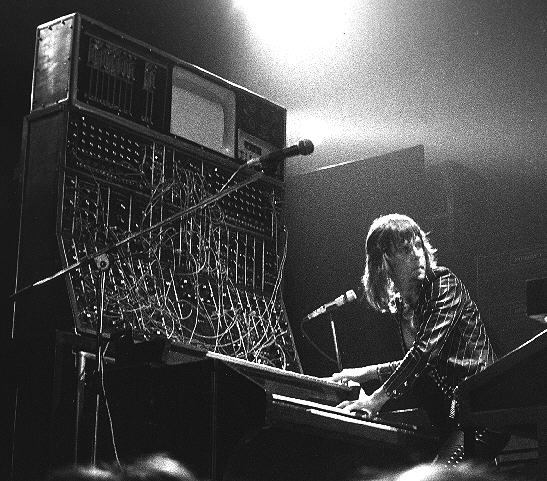
\includegraphics[width=.7\textwidth]{pic/elpmoog.jpg}
  \caption[Keith Emerson playing a modular Moog]{Keith Emerson playing
    a modular Moog. The keyboard is connected to a big rack of
    modules, interconnected with eachother with wires. Each module
    generates or processes the sound carried in analog form in the
    interconnecting wires, therefore having an exponential number of
    possibly different sounds by combining modules and settings.}
\end{figure}

After that, I started to listen to more and more music made with
electronic devices --- an exploration that happened, actually,
following electronic music's own history. From the synthesiser-full
rock of Soft Machine, King Crimson or The Nice I opened my ears to the
purely synthetic orchestral compositions of Wendy Carlos, Vangelis or
the early Jean Michelle Jarre. Kraftwerk's own evolution from rock to
drum-pads, vocoders and synthesisers allowed me to open my ears to
more modern electronic music.

\begin{figure}[h!]
  \begin{minipage}{\textwidth}
    \centering
  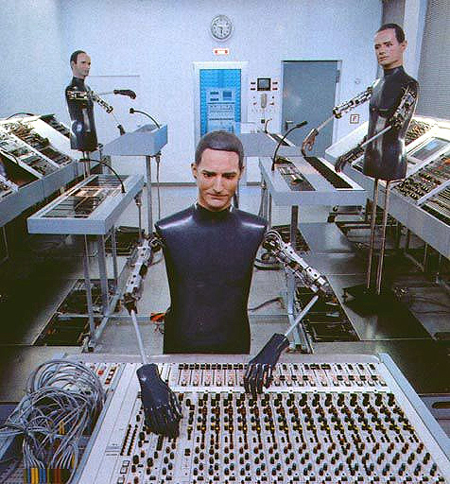
\includegraphics[width=.6\textwidth]{pic/kraftwerk.jpg}
  \caption[Artwork for the music of Kraftwerk]{Artwork for the music
    of Kraftwerk, with robotic representations of the band members
    playing with electronic instruments. On the front we can see an
    old analog sequencer.\footnote{As opposed to a synthesizer ---this is, a
    virtual instrument, which is in charge of producing sound of
    whatever note you tell it to--- a \emph{sequencer} is an
    electronic score that can not produce sound by itself. The notes
    are programmed in the device ---in an analog sequencer, by
    toggling switches and knobs--- and it sends them at the
    appropriate time and duration to the electronic instruments
    (synthresisers) it is connected to. While current digital
    sequencers are very powerful, at that time they had important
    limitations that influenced Kraftwerk's robotic but charm
    sound. Kraftwerk was one of the first pop bands to produce its
    music entirely with electronic devices and is considered the
    father of modern electro and techno and has heavily influenced
    many other styles like house and hip-hop.}}
  \end{minipage}
\end{figure}

It was still my first year of university when I watched a video, under
circumstances probably similar to that before, of a new device being
developed in the University Pompeu Fabra, in Barcelona: the ReacTable
\cite{jorda07thereactable}. In a dark room only illuminated by a
bright blue table, several performers placed tagged objects on the
table. The table automatically arranged a connection graph among the
objects based on their nature and relative distance and it displayed
it but, more interestingly, the sound was evolving as this graph
did. I just thought: wow, that must be fun, I want to play with that!
--- well, Do It Yourself.

That was the birth of Psychosynth. At the beginning it was just a
toy. I did know nothing on how to process real-time audio, so I wrote
many experiments. When I was bored of testing the dynamic range of my
speakers and ears with all sorts of sinusoids, triangle and square
signals I started to read more and more source code of other audio
Free Software and eventually started to write a digital modular
synthesizer and play with Ogre3D. %\cite{ogre3d}.
\footnote{Torus Knot Software Ltd. \url{http://www.ogre3d.com}} By the
summer of 2007 I had some very primitive synthesis code and also some
user interface experiments\footnote{As this video can show,
  \url{http://blip.tv/file/325103}, the software was just a bunch of
  buttons with a 3D blue table like Reactable's and no sound.}. While
I was an average C developer when I started my studies, I did not have
any clue on C++. During the development of these initial experiments,
I also had to learn about inheritance, what \texttt{virtual} means,
etc. but of course the design was flawed all the time and I had to
rewrite the code many times.

\begin{figure}
  \begin{minipage}{\textwidth}
    \centering
    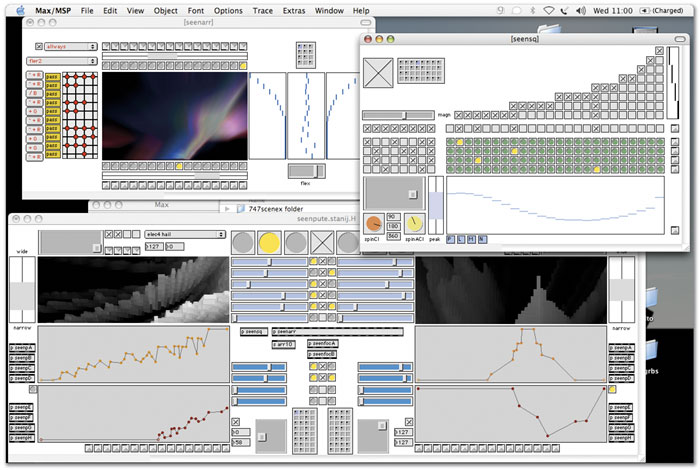
\includegraphics[width=.7\textwidth]{pic/autechre-2.jpg}
    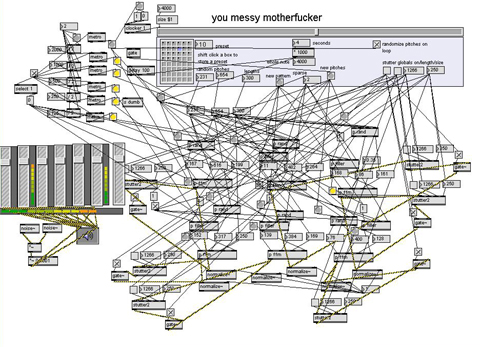
\includegraphics[width=.7\textwidth]{pic/autechre-1.jpg}
    \caption[Autechre related Max/MSP patches]{The first picture is a
      Max/MSP claimed to be made by the electronic music duo
      Autechre\cite{autechrepatch}. The second is a Max/MSP patch made
      by Robbie Martin that \emph{generatively} reverse-engineers Autechre's
      song Powmod.\footnote{Music is said to be \emph{generative} when the whole
        composition itself is performed by pseudo-random algorithms
        programmed to produce well-sounding evolving non-repeating
        patterns. Autechre are known to have explored generative
        music. Max/MSP and its Free Software counterpart Pure Data are
        graphical data-flow programming software, which can be considered
        a low-level modular synthesizer, that is often used to write
        arbitrarily complex musical software and is specially interesting
        for generative music.}}
  \end{minipage}
  \label{fig:autechre}
\end{figure}

Something happened then at the beginning of my second year of
university: I applied as a contestant to the Spanish Free Software
Contest for University Students, and Psychosynth was the project I
would develop. At that time I was already interested in experimental
electronic music from the 90's, and late programming nights were
accompanied by Autechre's fractal glitchs and Aphex Twin and
Squarepusher's spastic patterns\footnote{If there is something I am
  grateful for during the early development of Psychosynth is the
  patience of my flatmates during those noisy programming
  nights. Psychosynth was long-time nicknamed ``the ambulance siren
  sound maker'' because it was only able to produce recursively
  modulated sinusoids.}. At that time, this cruise in the most
experimental side of electronic music and my ignorance in proper music
making made me believe in scoreless generative music produced from
evolving continuous signals, and that influenced the lack of proper
synchronisation mechanisms in Psychosynth. At some point,
Shaker08\footnote{\url{http://soundcloud.com/shaker08}}, a music producer
and DJ from Malaga, developed some beat loops to distribute along with
the software and helped in early showcase performances. He also
tough me a lot on how music is traditionally made.

The project won a price in that Free Software contest and he got some
reviews in blogs. it then became part of the GNU project --- an
attempt to assure its long-term development and that it would remain
Free Software in the future.

After that, however, the development stalled a bit. I had big
refactoring ideas that never got the motivation to be accomplished. In
that seek for perfect code motivated by an increasing interest in
programming language theory and functional and generic programming, I
also became more and more conscious of the flaws of the code
---i.e. the lack of synchronisation mechanisms, MIDI (Music Instrument
Digital Interface) support, pluggable modules, patch persistence,
etc.\ make any serious non-experimental attempt to make music with it
very hard. During these last 2 years I have learnt much more on the
music production workflow and terminology, a process parallel to a
final step in opening my ears to current electronic music, specially
Drum and Bass, Dubstep, and even some Minimal and Techno. During last
summer I got a MIDI DJ controller that got me to better understand the
limitations and possibilities of Psychosynth for music mixing and I
became a casual contributor of the best Free Software DJ software:
Mixxx \cite{andersen03mixxx}. Also, the people at
ArtQuimia\footnote{\url{http://www.artquimia.net/}}, the music production
school where Shaker08 was educated, became interested in the project
and has offered lending gear for testing and supervision, guidelines
and insight from a musician point of view.

So here we are now, in the fall of 2010. Still quite ignorant in music
making but pretending to be a ``digital luthier'' motivated by passion
for music. And trying to turn all this personal game into a final
master thesis project. Lets see how it goes\ldots

\chapter{Introduction, definition and goals}

\epigraph{La utopía está en el horizonte. Camino dos pasos, ella se
  aleja dos pasos y el horizonte se corre diez pasos más
  allá. ¿Entonces para que sirve la utopía? Para eso, sirve para
  caminar.}{\textsc{Eduardo Galeano}}

\section{Problem definition}

Our problem definition is well expressed in the title of this project:
``a framework for modular, interactive and collaborative sound
synthesis and live music performance''. Lets elaborate this by
describing its parts.

\subsection{A modular synthesiser}
\label{sec:defmodular}
A modular synthesiser is one where the sound generation and
manipulation process is described as a directional graph where each
link represents the flow of sound signal from one node to another, and
each node transforms or generates those signals.

A node with no input is often called a \emph{generator}. A node with
one input and one output is often called a \emph{filter}. A node can
have different \emph{parameters} that in analog hardware can be set
with knobs and potentiometers. Often, these parameter can be
controlled with other optional input signals that are called
\emph{modulators}. A concrete interconnection of a set of modules is
commonly referred as a \emph{patch}. Note \ref{note:modsynth} lists
some of the most common modules in analog modular synthesisers.

\begin{mynote}[Standard modules in an analog modular synthresizer]
  \label{note:modsynth} Software modular synthesizers have usually
  similar ones in their default module too, while they quite often use
  different terminology not related to this voltage based signal like
  in this case.
  
  \noindent [The following text is extracted from the Wikipedia
  article on ``Modular Synthesizer,'' as checked on December 12th
  2010.]
 
  \begin{description}
  \item[VCO] Voltage Controlled Oscillator, which will output a
    pitched sound (frequency) in a simple waveform (most usually a
    square wave or a sawtooth wave, but also includes pulse,
    triangle and sine waves).
  \item[Noise source] A generator that supplies ``hiss'' sound similar
    to static, which can be used for explosions, cymbals, or
    randomly generated control signals. Common types of noise
    offered by modular synthesizers include white, pink, and low
    frequency noise.
  \item[VCF] Voltage Controlled Filter, which attenuates frequencies
    below (high-pass), above (low-pass) or both below and above
    (band-pass) a certain frequency. VCFs can also be configured to
    provide band-exclusion, whereby the high and low frequencies
    remain while the middle frequencies are removed.
  \item[VCA] Voltage Controlled Amplifier, which varies the
    amplitude of a signal in response to a supplied control voltage.
  \item[EG] Triggering an Envelope Generator produces a single,
    repeatable shaped voltage pulse. Often configured as ADSR
    (Attack, Decay, Sustain, Release) it provides the means to shape
    a recognizable sound from a raw waveform. This technique can be
    used to synthesize the natural decay of a piano, or the sharp
    attack of a trumpet. It can be triggered by a keyboard or by
    another module in the system. Usually it drives the output of a
    VCA or VCF, but the patchable structure of the synthesizer makes
    it possible to use the envelope generator to modulate other
    parameters such as the pitch or pulse width of the VCO. Simpler
    EGs (AD or AR) or more complex (DADSR—Delay, Attack, Decay,
    Sustain, Release) are sometimes available.
  \item[LFO] A Low Frequency Oscillator is similar to a VCO but it
    usually operates below 20 Hz. It is generally used as a control
    voltage for another module. For example, modulating a VCO will
    create vibrato while modulating a VCA will create tremolo.
  \item[RM] Ring modulator, two audio inputs are utilized to create
    sum and difference frequencies while suppressing the original
    signals. This gives the sound a ``robotic'' quality.
  \item[Mixer] A module that combines multiple signals into one.
  \item[S\&H] Sample and hold, which takes a ``sample'' of the input
    voltage when a trigger pulse is received and ``holds'' it until a
    subsequent trigger pulse is applied. The source is often taken
    from a noise generator.  Sequencer, which produces a sequence of
    notes, usually a music loop.
  \item[Slew limiter] Smooths off the peaks of voltages. This can be
    used to create glide or portamento between notes. Can also work
    as a primitive low-pass filter.
  \item[Custom Control Inputs] Because modular synthesizers have
    voltage-driven inputs, it is possible to connect almost any kind
    of control. Pitch can be varied by room temperature if you wish,
    or amplification varied by light level falling on a sensor.
  \end{description}
\end{mynote}

Analog modular synthesisers where invented in parallel 1968 by
R. A. Moog Co. and Buchla in 1963 \cite{moog1964voltage}. There, sound
signal is more often represented by oscillating voltage levels running
through wires ---the links--- and manipulated by analog signal processor
modules. Usually these modules where arranged in big racks.

One of the biggest problems of modular synthesisers is their limited
ability to cope with \emph{polyphony}. We say that a synthesiser is
polyphonic when several different notes can be played at the same
time. The basic implementation technique for this is to have several
copies of the synthesis logic ---each is called a \emph{voice}--- and
dispatch each keystroke to an unallocated voice (if present,
otherwise, some note priority logic is to be implemented). In old
analog modular synthesisers this was achieved by having multiple root
oscillators, maybe 2 or 4, but this multiplied the complexity of
connecting the synthesis graph. That is one of the main reasons why
modular synthesis was gradually abandoned for analog devices, as a
naturally sounding keyboard-controlled instrument should have a much
higher grade of polyphony and should remain usable ---note that the
required polyphony level is higher than the maximum number of keys that
we want to be able to press simultaneously, because a note remains
playing after the key is released during a \emph{decay time} while the
sound softly fades out.

Nowadays, the increasing power of computers allows us to build modular
synthesisers by software. Even further, we are no longer limited by
wires and we can use arbitrary data types as processing and
instantiate copies of the modules as we wish only constrained by our
memory and computation power. On software, it is easier to achieve
polyphony but it is still a non-trivial problem to make it
efficiently.

\subsection{An interactive synthesiser}

Even though Keith Emerson virtuously manipulated the wires and knobs
of his Moog in the middle of his performances, old-school modular
synthesisers have the inconvenience that they are rather static. It is
very hard to control all the parameters during the
performance. Changing the topology of the synthesis network is almost
impossible, and in most systems it causes clicks and other
inconvenient noises as a result of abruptly connecting and
disconnecting the wires ---whether software or analog.

We should design our engine with care so no noise is generated as a
result of manipulating the system live. But we should also provide
other means to enable easier manipulation of the topology.

\subsubsection{Dynamic patching}

The \emph{dynamic patching} \cite{kaltenbrunner04dynamic} technique
was first introduced in the ReacTable project and offers means to
automatically interconnect the modules of a software modular
synthesiser. When present, modules are laid out in a bi-dimensional
space and each output automatically connects to the nearest available
input of its same kind. The sink node that leads the output to the
speakers is situated in the centre and the synthesis graph grows as a
radial tree around it, as shown in figure \ref{fig:dynamicpatch}. By
simply moving one module from one position to another the user can
radically change the topology of the network without doing a lot of
plugging and unplugging of wires. A clever disposition of the modules
on the space can help the artist to achieve new innovative ways of
producing variations in his music.

\begin{figure}[h!]
\centering
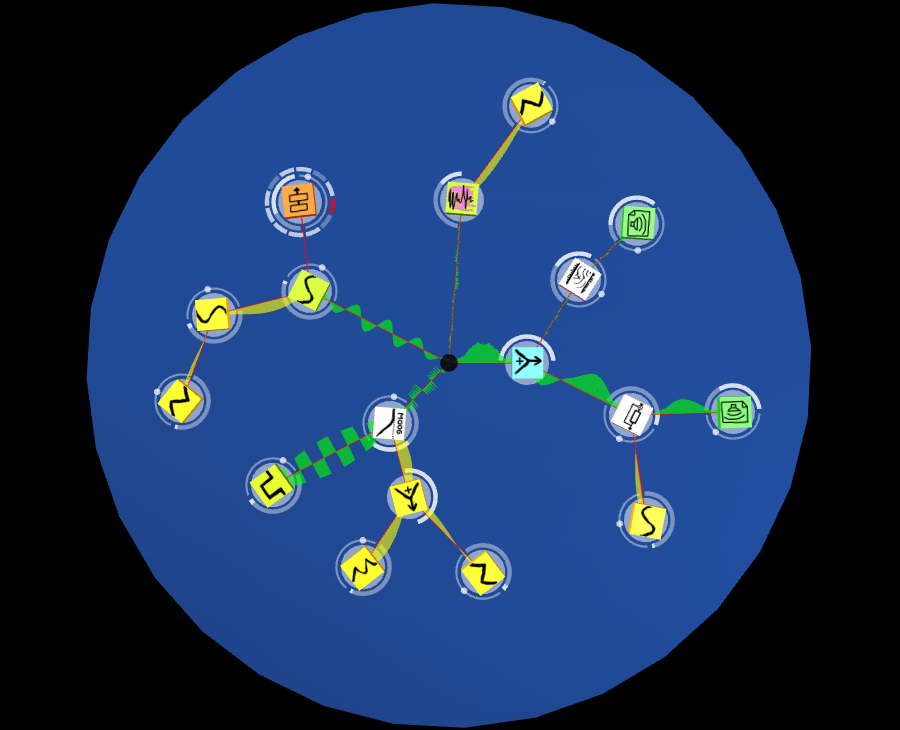
\includegraphics[width=.6\textwidth]{pic/dynamic-patch.png}
\caption{A screenshot of Psychosynth 0.1.1 using dynamic patching to
  connect a complex graph.}
\label{fig:dynamicpatch}
\end{figure}

\subsubsection{Touchable interfaces}

An specific problem for music software is that its interface is highly
limited by the keyboard and mouse as interface. While a person has 20
fingers\footnote{She must be very skilled to use all of them at the
  same time!} she is limited to manipulate only one parameter at a time
with the mouse.

There is an increasing availability of touchable interfaces, either
specifically designed for music performance like the Lemur (figure
\ref{fig:lemur}) or general purpose ones like the IPad. There, one is
no longer constrained by the single-click paradigm and not only can
she manipulate various parameters at a time, different multi-tap
gestures can expand the possibilities of a spatially limited user
interface as several functions can be reached in the same points.

\begin{figure}[h!]
\centering
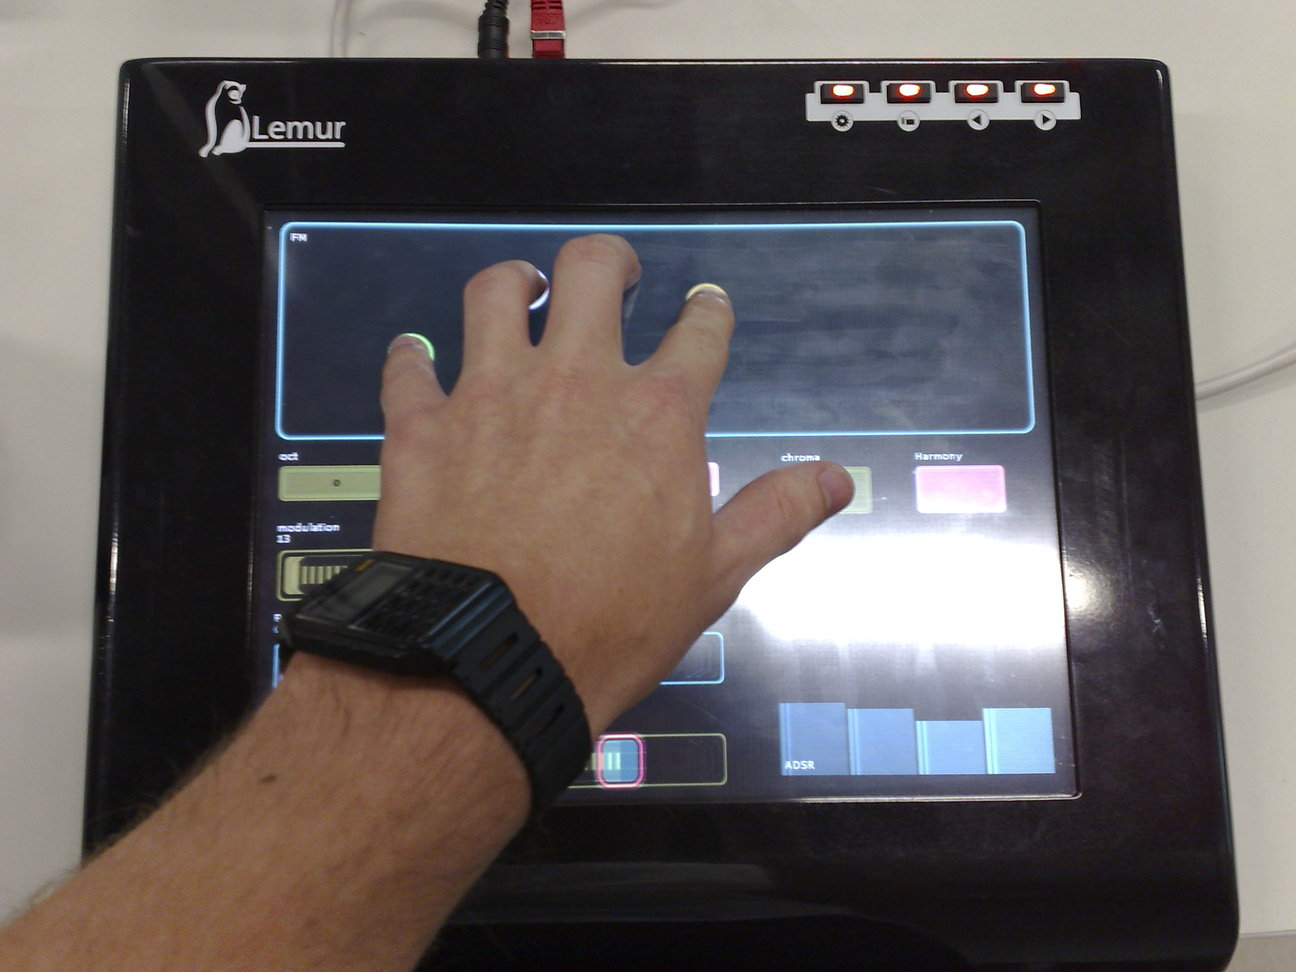
\includegraphics[width=.6\textwidth]{pic/lemur.jpg}
\caption[The JazzMutant's Lemur touchable music interface.]{The
  JazzMutant's Lemur touchable music interface. All the on-screen
  controls can be configured with an UI designer program, and later
  mapped to any program via OSC messages.}
\label{fig:lemur}
\end{figure}

\subsubsection{Instrument simulating controllers}

While touchable interfaces might be better for manipulating the
continuous parameters of the synthesis and dynamically manipulate a
sequencer, many musicians would prefer more traditional interfaces to
interpret part of their work in the ``old-fashioned'' way of playing
an instrument \cite{magnusson07acoustic}. There exists many kinds of
electronic devices that simulate the feel of a keyboard or a drum-kit
(figure \ref{fig:midicontrol}) but instead of producing any sound they
send MIDI \cite{completemidi} messages to a synthesiser that reproduces
the notes.

Our software should be able to interpret MIDI messages such that it
can be controlled with such a device, making it more natural and
creative for many musicians.

\begin{figure}[h!]
\centering
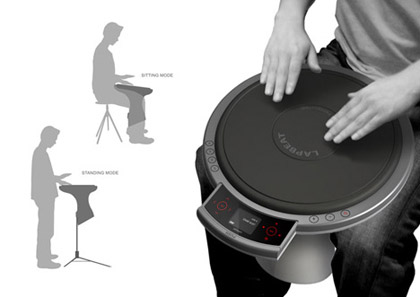
\includegraphics[width=.6\textwidth]{pic/lapbeat.jpg}
\caption[A conga-alike MIDI controller.]{A conga-alike MIDI
  controller. When pressing different parts of its surface it will
  emit different MIDI note messages, that a synthesiser or sampler
  could use to either simulate a real conga or to produce any other
  sound.}
\label{fig:midicontrol}
\end{figure}

\subsection{A collaborative environment}

Since the beginning of times, music performance have been a
collaborative act, with each performer contributing to the global
rhythm and harmony by playing one instrument. Psychosynth should serve
the purpose of producing arbitrarily complex music by itself as
modules that implement not only synthesis, but also sampling and
sequencing are added.

This integrated environment should be able to be manipulated by
several people at the same time to allow a collaborative
experience. After all, it would be very hard for one person to control
in a live performance all the subtleties of the sound generation by
herself.

\subsubsection{Tangible interfaces}

One approach to achieve this is by using a user interface that is big
enough to accommodate several performers around it. A tangible
interface is one where the different elements are represented by
physical objects that one can touch and move in physical space.  The
ReacTable implements such an interface where the modules of its
synthesis engine are plastic blocks that are laid out over a round
table that provides visual feedback thanks to a projector under it. As
shown in figure \ref{fig:reactable}, with such an intuitive and
physically unconstrained interface several people can stand around the
device and manipulate it.

\begin{figure}[h!]
\centering
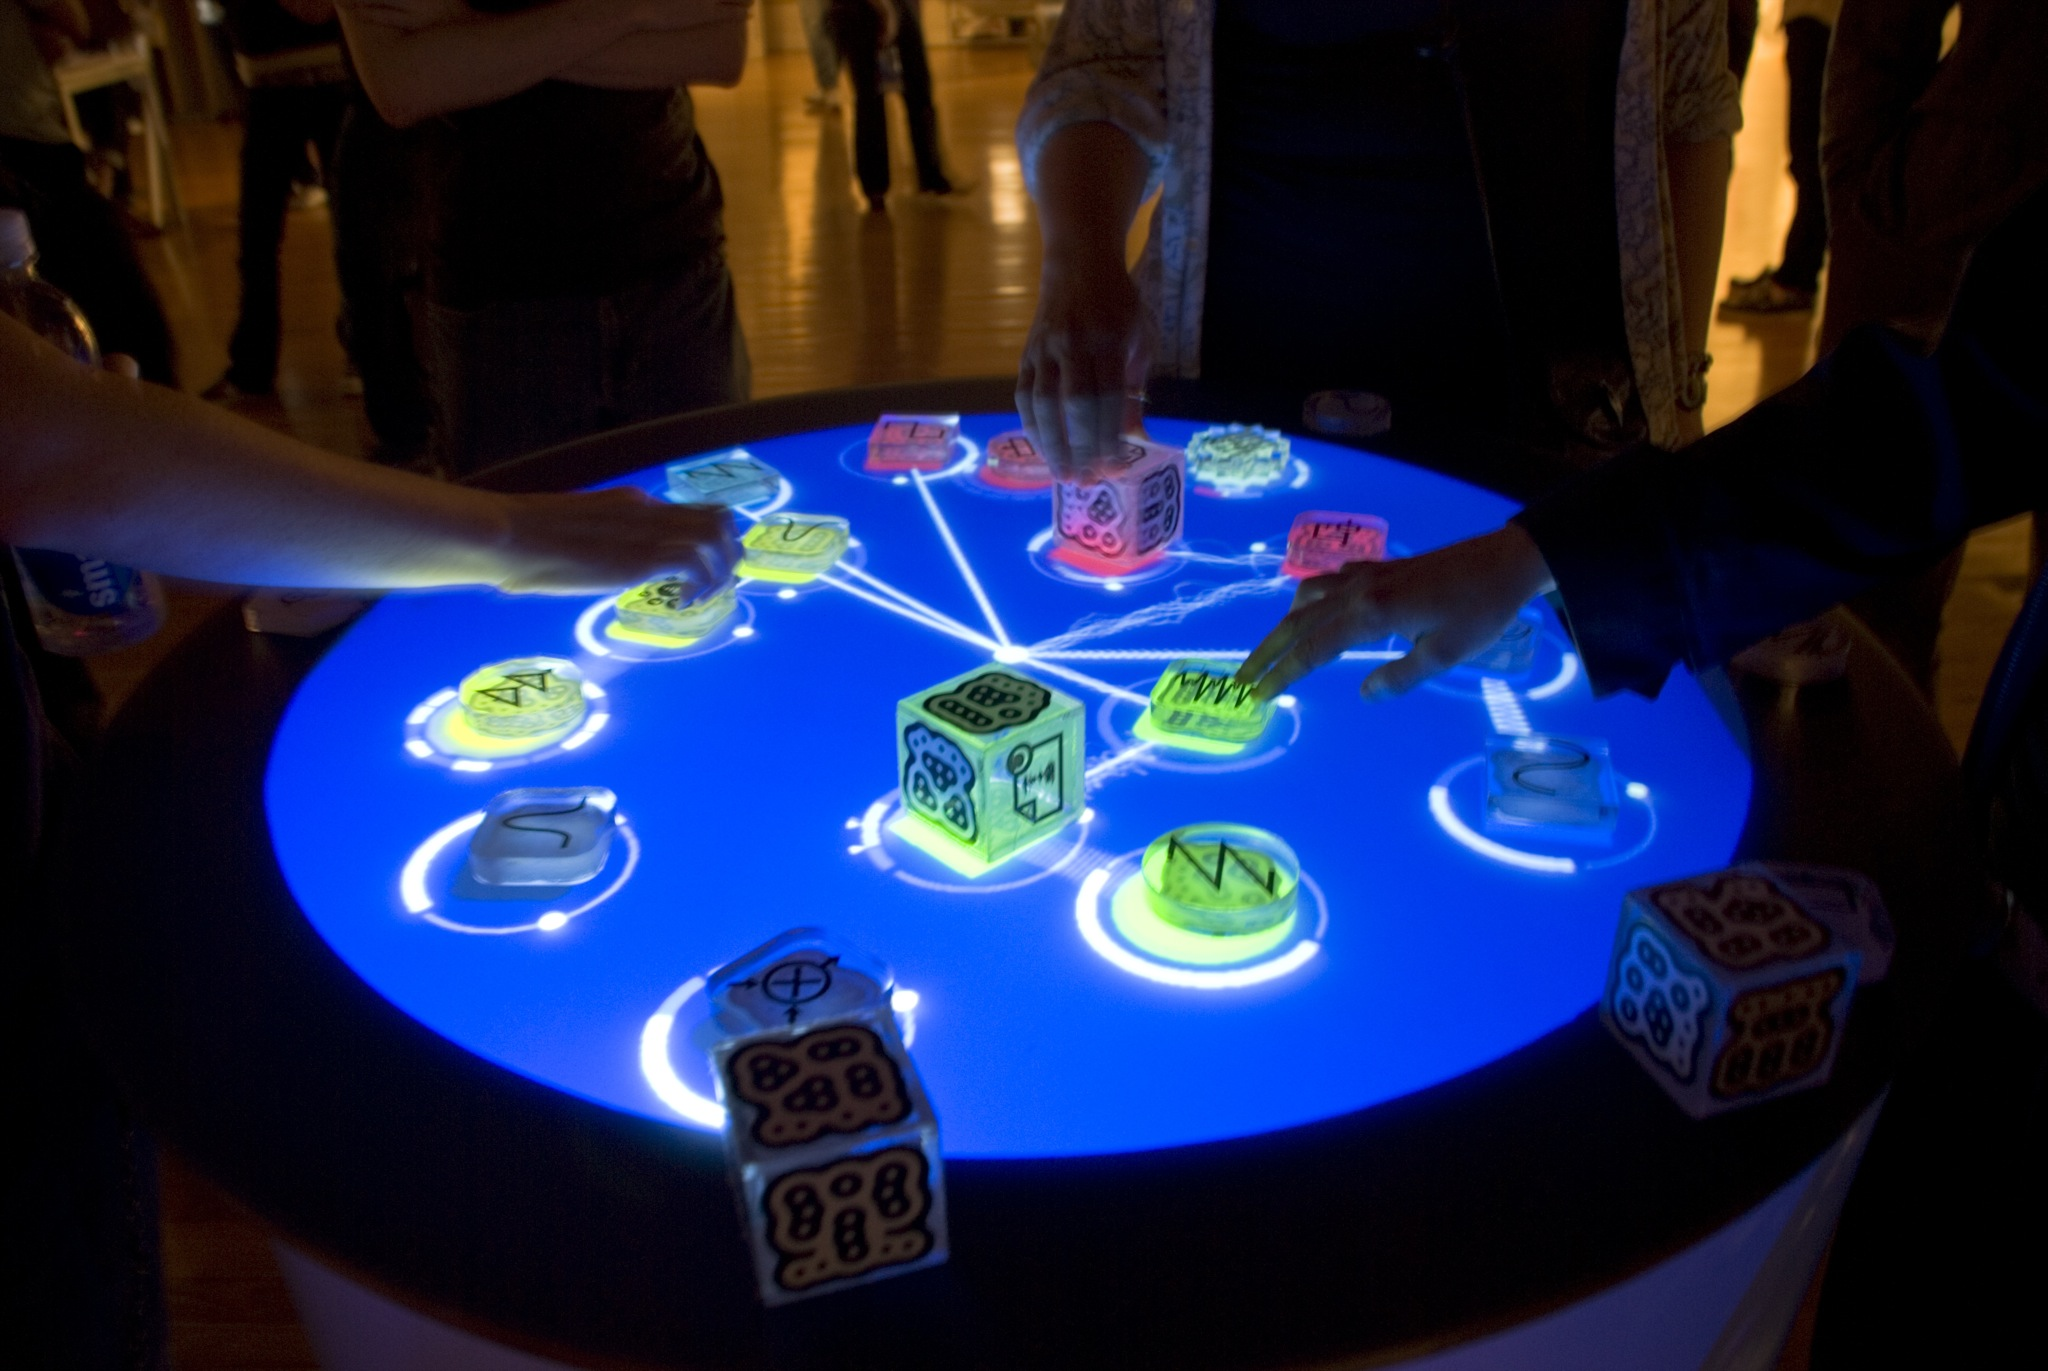
\includegraphics[width=.7\textwidth]{pic/reactable.jpg}
\caption{An example of the Reactable being used collaboratively by
  several people.}
\label{fig:reactable}
\end{figure}

\subsubsection{Networking}

Networking support even further releases a device from the space
constraint by allowing several instances of the software
intercommunicate over a computer network ---i.e. IP. At some point,
latency problems can still be a drawback for this technique, but it
can be useful for some kinds of collaboration that do not require
perfect timing. When playing in a local range, this becomes perfectly
valid even under high latency requirements.

This has long time been a main goal in Psychosynth. When running in
collaborative mode, all the clients that connect to a server share the
same synthesis graph and whenever and object is moved, added or
deleted, or a parameter is changed, all are notified such that they
keep the same view of the scene. Figure \ref{fig:collab} shows an
example of this feature being used live.

\begin{figure}[h!]
\centering
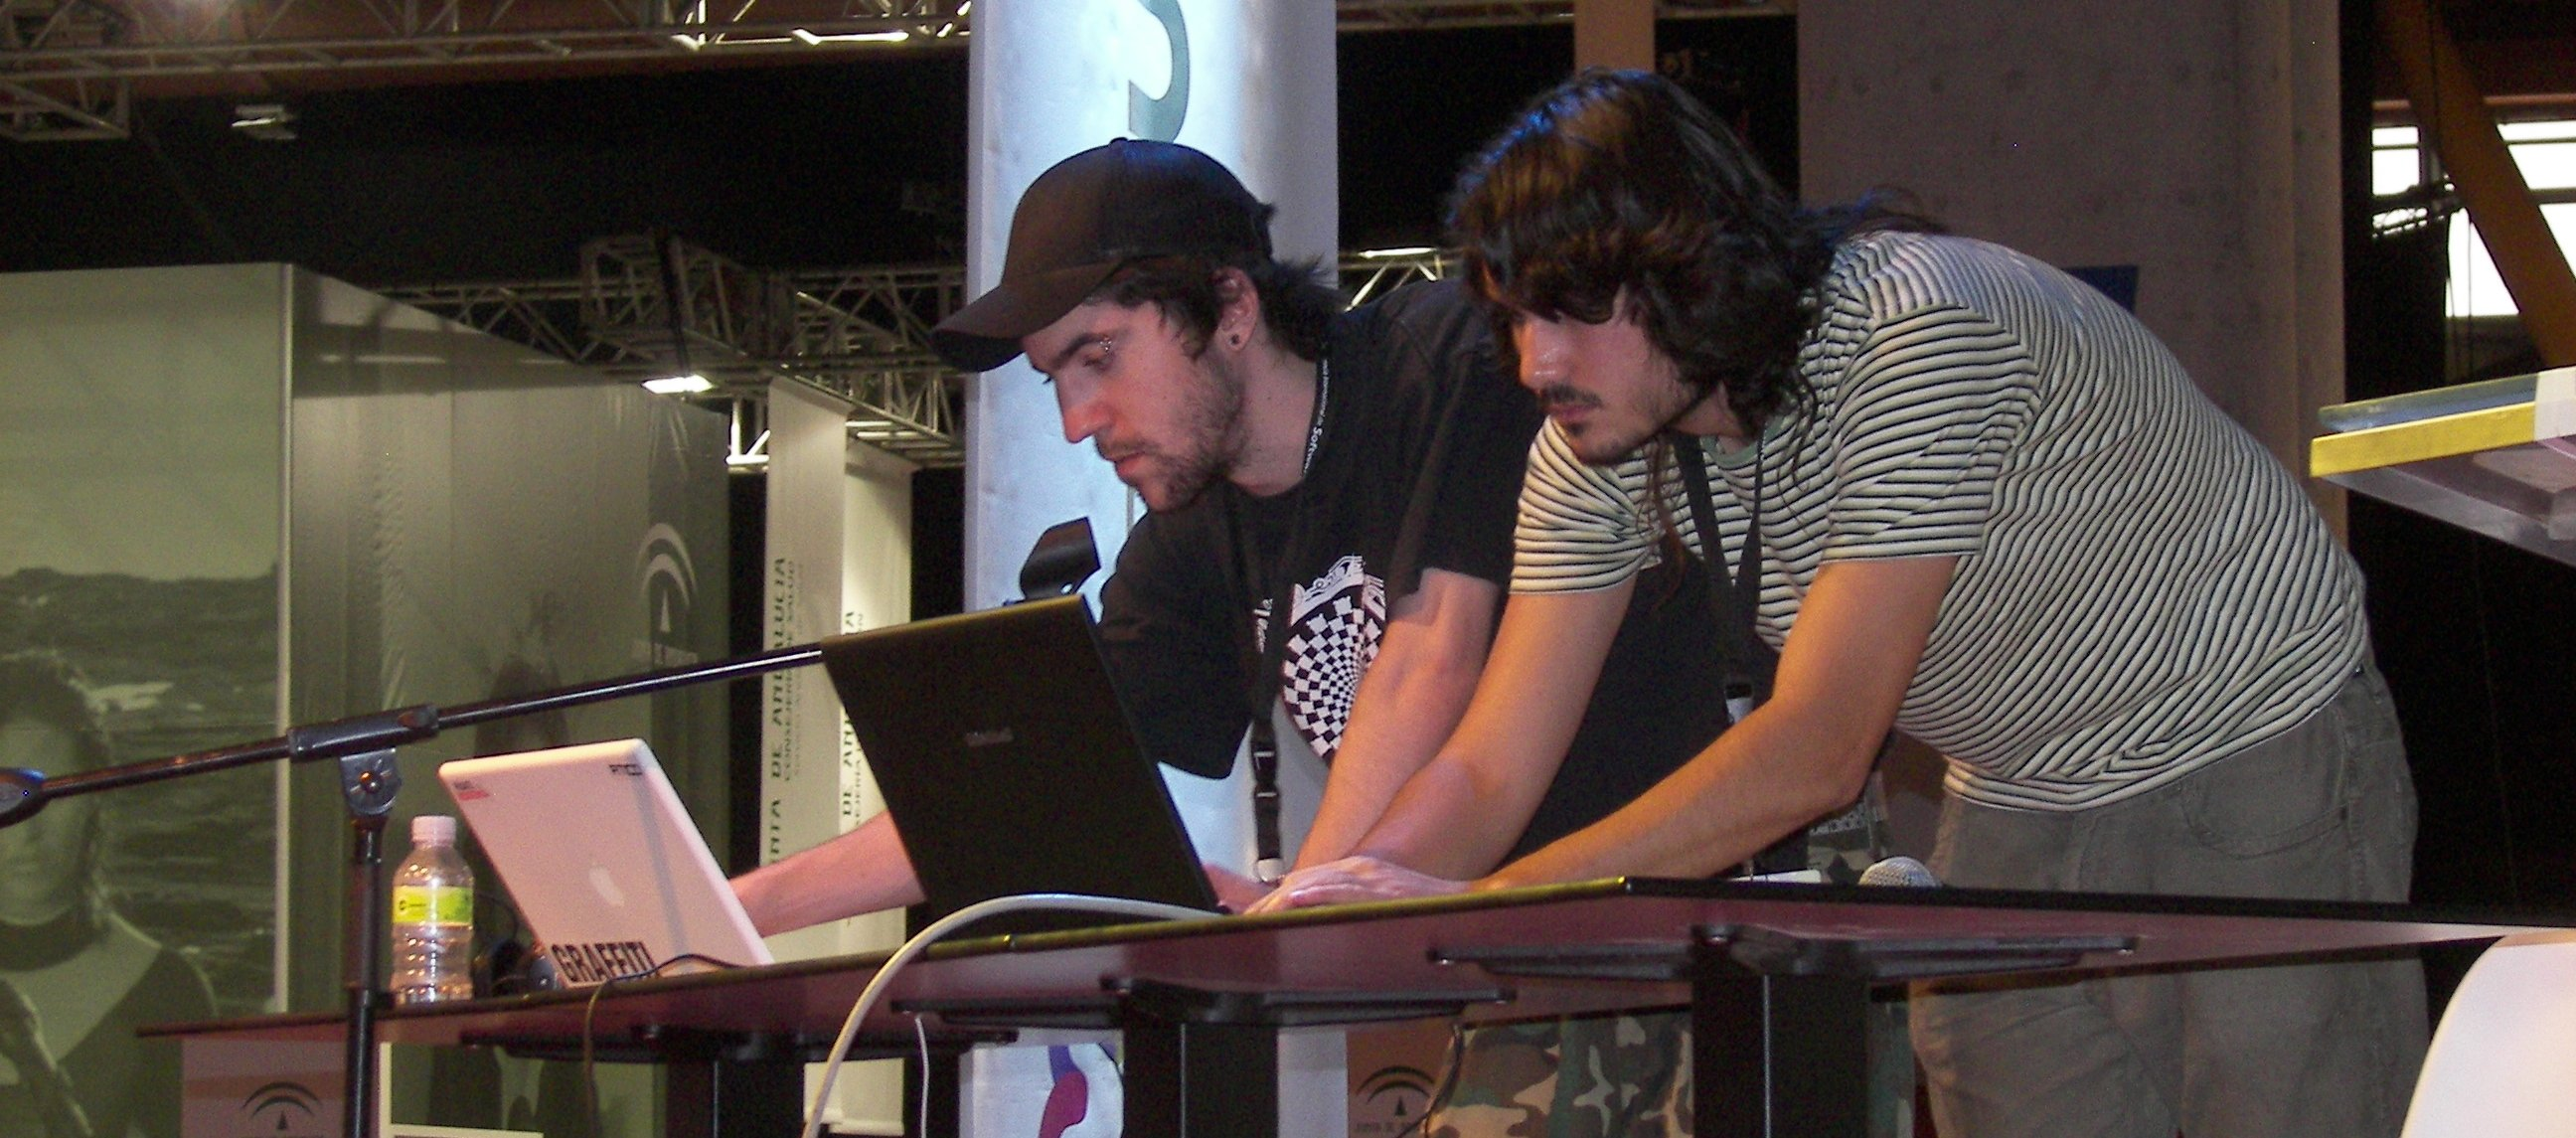
\includegraphics[width=.9\textwidth]{pic/collab.jpg}
\caption[An example of Psychosynth 0.1.4 being used collaboratively
over the network.]{An example of Psychosynth 0.1.4 being used
  collaboratively over the network. The picture was taken in a
  showcase performance held by Shaker08 and the author in the Open
  Source World Conference in 2008.}
\label{fig:collab}
\end{figure}

\subsection{A framework}

Music making and audio processing software and interfaces are evolving
very fast. Abstracting the common core functionality needed by
developers in a layered and abstracted programming API and development
of a Free Software \cite{stallman2002free} framework is crucial to enable
further focused research on the different areas previously
discussed. Results of that research can be later integrated in the
framework as they are stabilised.

Such a framework should enable the development of modular audio
applications with an abstracted interfacing mechanism, probably
following a Model-View-Controller paradigm, general enough to be able
to support all the previously described qualities. If this task is
properly accomplished, the framework could become the basis of a wide
range of unexpected future Free Software applications.

\section{Objectives}

Taking all that into account, we should next define the concrete
objectives for our present project. We should note that we depart from
the basis of the current state of the GNU Psychosynth project ---as of
its version 0.1.7--- and we assume that as previous work, not our
current target.

\subsection{Main objective}
\label{sec:mainobjective}
\label{sec:userinterface}

\begin{objective}
  Re-focus the GNU Psychosynth project as a development framework for
  the development of professional-quality modular, interactive and
  collaborative synthesisers.
\end{objective}

In the long-term we would like GNU Psychosynth to include innovative
user interfaces, and some might even be developed as a side effect of
this project ---or we might just update the older one to rely on the
new framework. However, that is not the purpose of this project,
instead we will concentrate on the development of the underlying core
architecture and implementation of its API.

This is so mainly because of time constraints. Also, if we were to
miss some features in the core in order to allocate more time for the
user interface, we have to take into account that this will probably
hard to fix afterwards when a lot of code depends on the broken
design. Also, user interface development is easier to do in a
non-disciplined, voluntary and heterogeneous team. If we achieve a
nice framework now we can still develop the user interfaces later with
the help of other the people collaborating on the Internet; but, as
these two years of stalled development have shown, it is hard without
the pressure of an external deadline and a project plan to invest a
lot of time in rewriting the ``invisible'' but crucial parts of the
system.

\subsection{Preconditional objectives}

There are two objectives of this project that can also be considered
as a precondition for the success of our main goal. These are:

\begin{objective} \label{obj:artquimia}
Collaborate with professional musicians to get a
defined understanding of the meaning of ``professional quality'' and
their real needs.
\end{objective}

The students participating is this project have an amateur knowledge of
music production. It is important to communicate and allow supervision
by professional musicians and experts in digital music to assure the
suitability of the software for use in a professional environment.

We are working in collaboration with the ArtQuimia Music Production
School\footnote{\url{http://www.artquimia.net/}}, which has long time
been educating successful producers and is currently participating in
the European Cross-Step
project\footnote{\url{http://www.cross-step.org/node/4}}, and his
director David García, a musician with professional experience in the
industry as music composer and sound designer for video games.

\begin{objective}
  Research and apply the latest techniques in modular design and
  implementation and explore the boundaries of the underlying
  implementation devices.
\end{objective}

The success of an framework relies on the proper decomposition of its
features and its extensibility. Moreover, the authors of this project
have a special fascination for programming languages, design patterns
and software modularity. Even more, there is an active research
community questioning and re-developing the modularisation and
abstraction techniques of the underlying programming language C++,
a fact that is more true as we approach the final resolution of the
standarisation committee on the new C++0x standard. All this suggests
that research and application of the state-of-the-art and even
development of our new design and coding patterns will be one of the
leading objectives during the project and play a leading role in
its overall success.

\subsection{Partial objectives}

A more concrete subdivision of our main goal should be given. Note
that these are not yet the detailed requirements, but an overall
initial objectives vaguely elicited from the problem definition, the
previous experience with the GNU Psychosynth software and our personal
interests.

\begin{objective}
Improve the framework to be able to load modules dynamically from
plug-ins, satisfying our own API and/or third-party standards.
\end{objective}

This is a common feature in most industry standard applications and
ours should support it. Many layers of the framework, specially those
related to the dynamic patching, will require vast modifications to
enable customisation to understand third-party modules.

\begin{objective}
Improve the framework to be able to communicate with music controllers
via MIDI or other industry standards.
\end{objective}

While not explicit in this wording, this adds the requirement for
\emph{polyphony} as in most cases such feature would be useless without
it.

\begin{objective}
Add basic synchronization and sequencing support to the framework.
\end{objective}

If we want to understand the software as a full live performance
environment and not a bare synthesiser, this currently lacking feature
is fundamental.

\begin{objective}
Include common modular audio system utilities into the framework. Some
of the most important being patch hierarchy and persistence. 
\end{objective}


\section{Background and state of the art}

\subsection{Modular synthesis}

The history of modular audio generation starts with the Moog
analog synthesiser in 1967 \cite{moog1964voltage}. Since then, a wide
variety of analog modular synthesisers have been developed
commercially, but retaining some limitations as described in the
introduction in section \ref{sec:defmodular}.

Modular synthesis became more interesting with the uprising of
computer based electronic music. One of the most important examples in
this development is Max/MSP \cite{puckete2002max}. This is a dataflow
based visual programming environment mainly targeted at music
applications. In such software one can add boxes where one types the
name of the function that it should perform. When the name has been
written some connection plugs appear on its corners depending on the
module name, and one can draw lines connecting those plugs. Figure
\ref{fig:autechre} showed an example of its functioning. The author of
Max/MSP later developed a Free Software counterpart called Pure
Data\cite{puckette96puredata} that also has video processing
and synthesis support.

Since then, many user-oriented commercial modular synthesisers have
been developed. One of the most famous ones is Native Instrument's
Reaktor (figure \ref{fig:reaktor}). In its version 5 it included the
new \emph{core-cell} technology, which allows the visual and modular
design of the lower level parts of the DSP (Digital Signal
Processing) programming, which transparently compiled to efficient
machine code. Later, Plogue's Bidule is gaining special recognition
for its simpler interface. A new interesting software is XT Software's
EnergyXT, a DAW (Digital Audio Workstation) that has a ``modular
view'' where one can route through wires all the MIDI and audio
signals that flow behind the traditional sequencing view. Finally,
Sensomusic's Usine is remarkable for introducing a highly customisable
multitouch graphical interface on top of a modular synthesis
environment.

\begin{figure}[h!]
\centering
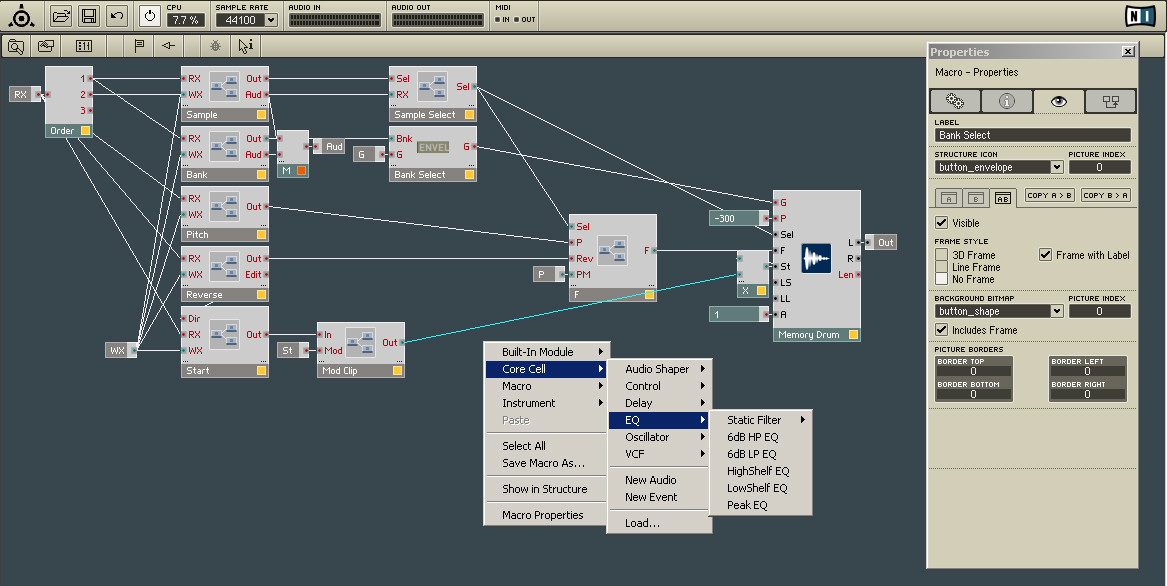
\includegraphics[width=.9\textwidth]{pic/reaktor.jpg}
\caption{Native Instrument's Reaktor editing a \emph{core cell} based
  patch.}
\label{fig:reaktor}
\end{figure}

On the Free Software side few modular synthesisers exist. Alsa Modular
Synth\footnote{\url{http://alsamodular.sourceforge.net/}} is one of
the most
popular. Ingen\footnote{\url{http://drobilla.net/blog/software/ingen/}}
is a more modern one whose code we praise for its quality. Most of
these software still lack some of the features of their privative
counterparts, with the ability to create customised user interfaces
being the most relevant. Still, Free Software offers a very
interesting modular approach to the sound system management that has a
similar rival only in latest OSX versions:
Jack\cite{letz09jack2}. Jack is an audio server providing zero-latency
interprocess communication that acts as a patch-bay among any
supporting audio applications. The user can route the output of one
program to the input of any other program, or the soundcard sink, or
whatever exposes a Jack port. It can be used to route MIDI signals too
and recent versions include very nice features, like collaborative
routing over the network for distributed performances \cite{hohn09netjack}.

\subsection{Touchable and tangible interfaces}

In the last decade, the development of touchable and tangible user
interfaces have been of rising interest. An interesting but not very
updated survey that gives some taxonomical background and analyses a
wide variety of products can be found here
\cite{blaine2003contexts}. One of the first attempts in using them for
improved interaction in musical software is the Audio
Pad\cite{patten2002audiopad}, where the user places and moves tagged
pucks on a bidimensional surface. This is an example of an interface
with active tangibles, because the pucks have an RF transmitter to
allow their recognition. The Jam-o-Drum, on the other hand, offered a
percussive collaborative approach where performers sit on the corner
of an interactive table \cite{blaine00jam}. Many videogames and other
kinds of application have been developed on top of the Jam-o-Drum
hardware too. Since then, a huge number of different table based
interfaces have been made, an example listing can be found
here\footnote{\url{http://mtg.upf.edu/reactable/related.htm}}.

Maybe the most interesting example, which inspired the whole
development of GNU Psychosynth, is the Reactable
project\cite{jorda07thereactable}. Its user interface is based on
modular synthesis and uses the dynamic patching technique for easily
manipulating the patch topology. It uses innovative digital image
processing techniques to detect the position and rotation of passive
tangibles \cite{bencina06improved}. In the Reactable system a
translucid round surface hides a projector and a high resolution
camera underneath, as shown in figure
\ref{fig:reactablesetup}. Finger-tips and the specially designed tags
called \emph{fiducials} that are placed on the table surface are
captured by the camera and recognised by the ReacTIVIsion system on a
computer. This system sends OSC\cite{center03osc} (Open Sound Control) based
messages to a synthesiser following the TUIO (Tangible User Interface
OSC) protocol \cite{kaltenbrunner05tuio}. The literature describing
the initial prototypes used Pure Data as the underlying implementation
language for this synthesis engine, but conversations with the authors
of the Reactable suggest that the current commercial implementation
is written in C++. This synthesis engine is connected to a visual
engine that generates visual feedback and sends it through the
projector. The picture is reversed so it can be correctly visualised
through the translucid surface.

\begin{figure}[h!]
\centering
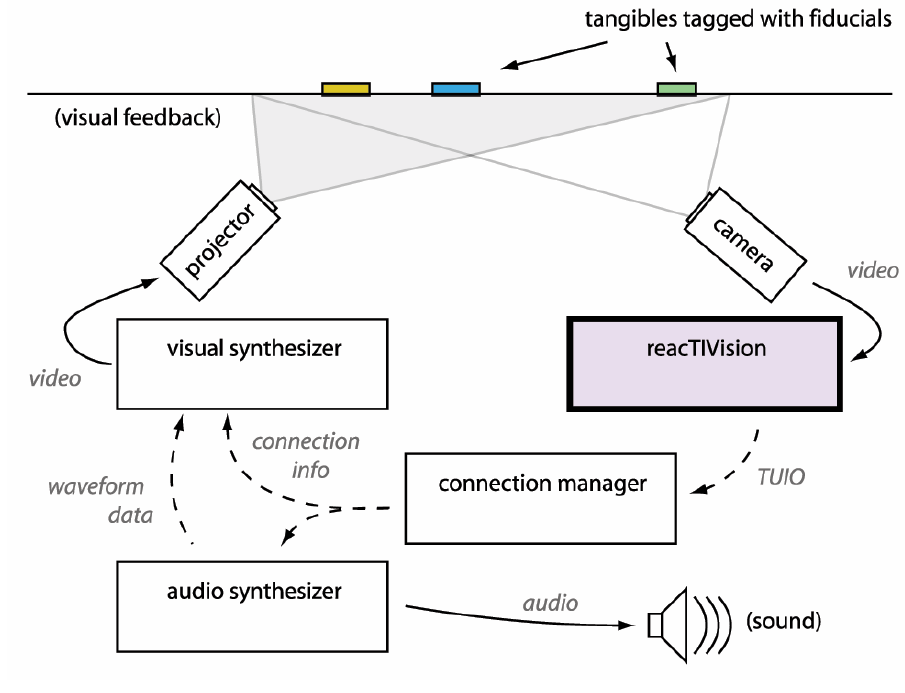
\includegraphics[width=.7\textwidth]{pic/reactable-setup.png}
\caption[A typical Reactable setup.]{A typical Reactable
  setup. Source: The Reactable project.}
\label{fig:reactablesetup}
\end{figure}

The Reactable has been very successful and a very interesting fact is
that the computer vision component of the system is Free Software, so it
could be integrated with GNU Psychosynth in the future.

Some other remarkable tangible and highly interactive user interfaces
that where released around 2007 too are the JazzMutant's Lemur and the
Iwai-Yamaha’s Tenori-On \cite{nishibori06tenorion}. The former offers
a fully customisable OSC based multi-touch interface, where one can
design interfaces with sliders, virtual-knobs, X-Y pads and all kinds
of multi-touch controls that are mapped to OSC messages that can be
interpreted by the audio engine of choice. The later is a 16x16 matrix
of LED illuminated buttons that can be configured in different modes
that provide innovative sequencing mechanisms (figure
\ref{fig:tenorion}).

\begin{figure}[h!]
\centering
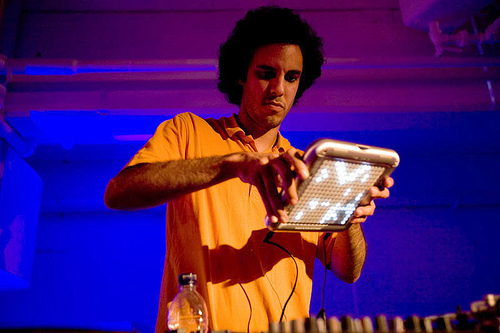
\includegraphics[width=.7\textwidth]{pic/tenorion.jpg}
\caption{Electronic music artist Four Tet performing with a Tenori-On}
\label{fig:tenorion}
\end{figure}

Nowadays, multitouch interfaces are the main trend, specially after
the explosion of the tablet market, but big music software companies
still have to catch up the latest hardware developments. Specially
interesting for the GNU Psychosynth projects it the Indamixxx 2
tablet, which is based on the Meego OS\footnote{Nokia and Intel's
  joint effort to provide a GNU/Linux based operating system for
  embedded devices, mobile phones, netbooks and tablets.} and oriented
towards music production and live performance --- we should definitely
keep an eye on it and develop a multi-touch enabled user interface for
it.

\subsection{Audio synthesis libraries and frameworks}
\label{sec:dsl}

One of the first synthesis libraries that where evaluated before the
development of GNU Psychosynth started is the STK (Synthesis ToolKit)
\cite{scavone05rtmidi} but it lacks proper dynamic signal routing
mechanisms and some details, like the sample format being hard-coded
to float, seem too constrained.

A popular sound synthesis and music composition DSL (Domain Specific
Language) is CSound, which later was extended with a C and C++
programming API\cite{boulanger00csound}. Many DSP oriented DSLs have
been developed, but they are not general enough to support the
development of the fully featured applications that we wish on top of
GNU Psychosynth. Still, some of them are worth mentioning. Notable
examples are SoundCollider \cite{mccartney2002supercollider}, which
was for a long time the reference sound synthesis DSL; Chuck
\cite{wang03chuck}, that adds concurrency and time control in an
elegant and boilerplate-less fashion, and the newer Faust
\cite{orlarey09faust}, which is based in a functional and data-flow
paradigm and interfaces easily due to its compilation to C++.

While we are focusing on C and C++, many languages have music related
libraries. Impromptu\footnote{\url{http://impromptu.moso.com.au}} is a
Scheme environment for live-coding, this is, live music performances
where the programming is done in front of the audience while the
programmer writes and mutates the code\footnote{The video
  \emph{Algorithms are thoughts, chainsaws are tools}, by Stephen
  Ramsay is a great introduction to this
  technique. \\\url{http://createdigitalmusic.com/2010/07/thought-and-performance-live-coding-music-explained-to-anyone-really/}}. It
supports video manipulation too, but sadly is available for OSX
only. Its heavy modularity and dynamism is what make Lisp dialects so
interesting for live-coding and music composition. Common
Music\cite{taube97common} was started in 1989 and it is a highly
featured Common Lisp framework that, among other things, provides a
very elegant embedded score notation.

Maybe the most similar project to GNU Psychosynth in its approach is
CLAM (C++ Library for Audio and Music) and award winning library based
on modular synthesis\cite{amatriain2006clam}. Its design will be
carefully taken into account during the redesign of few of Psychosynth
core components. Still it does not precisely fit our needs as it is too
oriented toward research simulations and does not support polyphony.


%%% Local Variables: 
%%% mode: latex 
%%% TeX-master: "00-main"
%%% End: 


\chapter{Analysis and planning}

\epigraph{As I see it, criticism is the prime \emph{duty} of the
  scientist and of anyone who wants to advance knowledge. Seeing new
  problems and having new ideas, on the other hand, are \emph{not}
  one's duty: originality is, rather, a gift of the gods.}{
  1982 Preface to \emph{Quantum theory and the schism in physics}\\
  \textsc{Karl Popper}}

\section{Requirement modelling}
\label{sec:requirements}

In the following section we discuss the requirements that we want to
impose on the resulting framework. Note that functional requirements
are hard to express for an API, but a vague description of the desired
qualities and features is still possible will guide or development
process.

Quite often, we will focus on the final feature that should be
implementable through the framework. Also, note that the framework
already had many features at the beginning of the project, some of
which we will discuss in section \ref{sec:status}. We will try to
avoid describing the requirements related to those ready facilities in
this section, as the only purpose of those is to aid the actual
development of this thesis project. Still, some already satisfied
requirements might be made explicit when some other related
requirement follows, or because of their relevance to the user or just
for the global consistency of the text.

As we suggested in our objective \ref{obj:artquimia}, these
requirements have been elicited with the assistance of the ArtQuimia
Music Production School in order to ensure the suitability of the
software in a productive usage context.

\subsection{Functional requirements}

\subsubsection{Basic audio support}

\begin{requirement}
  \label{req:iter1-begin}
  The library must provide data-structures and basic algorithms for
  manipulating audio signals.
\end{requirement}

\begin{requirement}
  The library must provide means to output and input audio data to and
  from files in various formats, including, at least: Microsoft WAV,
  Apple AU and OGG Vorbis.
\end{requirement}

\begin{requirement}
  \label{req:soundsys}
  \label{req:iter1-end}
  The library must provide means to output and input audio data to and
  from sound-card devices in an asynchronous real-time fashion,
  supporting, at least, the following audio systems:
  ALSA\footnote{Advanced Linux Sound Architecture:
    \url{http://www.alsa-project.org/}}, OSS\footnote{Open Sound
    System: \url{http://www.opensound.com/}},
  Jack\footnote{\url{http://jackaudio.org/}}.
\end{requirement}

\subsubsection{Node graph support}

\begin{requirement}
  \label{req:iter2-begin}
  The library must include means for producing the audio as the result
  of executing a dataflow-graph.
\end{requirement}

\begin{requirement}
  The library user must be able to define his own processing nodes.
\end{requirement}

\begin{requirement}
  \label{req:porttype}
  Each node should have an arbitrary number of named signal and
  control input and output ports. The difference between signal and
  control ports are that the later are sampled at much less frequency.
\end{requirement}

\begin{requirement}
  Both signal and control ports should be able to process information
  in arbitrary datatypes. Signal ports may have practical limitations
  as for the real-time constraints is concerned.
\end{requirement}

\begin{mynote}[Realtime constraints] \label{note:realtime} All the
  processing done inside the nodes should satisfy soft real-time
  constraints. This is so because in order to produce sound with low
  latency (see requirement \ref{req:latency}) the sound processing
  should be done in blocks (buffers) as small as possible that are
  delivered to the sound-card as soon as possible. If the deadline is
  not met, a disturbing ``click'' sound will be heard because of the
  zeroes assumed by the sound-card during the period that it did not
  have any audio to output. For example, for a 44100 Hz sampling rate
  and a 128 frames block size, it should take less than $$\frac{1
    s}{44100\ frames}\cdot128\frac{frames}{block}=2.90
  \frac{ms}{block}$$ to process and deliver an audio data block.

  In practice, this means that the processing algorithms should take
  an amount of time proportional to the amount of data to process
  ---i.e. they are $O(n)$. This in turn disallows writing and reading
  files and most operations that cause non deterministic hardware
  operations or force context switching (mutexes might be unavoidable
  but should be used scarcely). Also, allocation of memory on the
  heap should be avoided as it has a non-predictable and potentially
  non-linear time consumption. Of course, the framework should provide
  hooks to do those forbidden operations outside the audio processing
  thread, but we consider that a design issue that should be addressed
  later.
\end{mynote}

\begin{requirement}
Each output port must be connectable to arbitrary number of input
ports. Each input port must be connectable to one output port.
\end{requirement}

\begin{requirement}
Ports may be defined statically ---i.e. at compile time--- or
dynamically ---i.e. at runtime.
\end{requirement}

\begin{requirement}
The system must allow the hierarchical composition of nodes, with
special \emph{input} and \emph{output} nodes that are exposed as ports
in the parent level.
\end{requirement}

\begin{requirement}
\label{req:iter2-end}
Nodes can be either monophonic or polyphonic. A polyphonic node
internally has a number of copies of its processing state, called
\emph{voices}, that are dispatched accordingly trough trigger signals.
\end{requirement}

\begin{mynote}[On the scope of polyphony]
We will avoid specifying here details on how polyphony works that are
still quite important as a \emph{usability} concern. For example,
should monophonic ports be connectable to and from polyphonic ports?
Should there be polyphonic and monophonic nodes in the same patch
hierarchy level? How are the voices dispatched and mixed? Because
answering this issue highly affects performance and implementability
tradeoffs, these issues are left open until the design stage of these
components.
\end{mynote}

\subsubsection{Dynamic loading of nodes}

\begin{requirement}
  \label{req:iter3-begin}
  The system must be able to dynamically load modules developed with
  standard interfaces, at least using the LADSPA
  standard\footnote{Linux Audio Developer's Simple Plugin:
    \url{http://www.ladspa.org/}}, but LV2\footnote{LADSPA Version 2:
    \url{http://lv2plug.in}} and VST\footnote{Steinberg's Virtual
    Studio Technology: \url{http://ygrabit.steinberg.de/}} are
  proposed too in this order of priority. Note that in some cases this
  implies the automatic fixing of the semantic impedance among the
  interfaces of Psychosynth nodes and the third-parties'.
\end{requirement}

\begin{requirement}
  The system should be able to dynamically load modules developed
  using the same native interface exposed to library users to define
  their own modules. 
\end{requirement}

\subsubsection{Dynamic patching}

\begin{requirement}
  The system should optionally release the library user from arranging
  the interconnections among nodes by using \emph{dynamic
    patching}. When using \emph{dynamic patching} an output port is
  connected to one input port. The input port is the closest (in the
  sense of euclidean distance, we assume that the modules are laid out
  in the space) input port of the same type not belonging to the same
  node that is free ---i.e. is not connected already to a closer node.
\end{requirement}


When combining dynamic-patching with dynamically loaded modules
using standard interfaces like LADSPA, one might need extra
information to correctly perform the dynamic patching.

\begin{requirement}
  \label{req:iter3-end}
The system should be able to locate and automatically load if present
special description files containing the required information for
some dynamically loaded modules to work correctly. This file should
specify which ports are eligible and to which ports they are
connectable to. 
\end{requirement}

While this may change due to design considerations, we suggest
specifying a set of tags for each port, with the following
connectability rule for port $A$ and $B$: $connectable(A, B)
\Rightarrow tags(A) \cap tags(B) \neq \emptyset$. 

\subsubsection{View independence}

The following requirements are here to suggest an observable interface
for the synthesis model satisfying a model-view-controller
architecture. This is one of the key concepts in achieving a
network-based shared environment that is transparent to a wide range
of graphical interface experiments or external MIDI controls.

\begin{requirement}
  \label{req:views}
  The system must enable the development of graphical interfaces
  ---or any other instance of the more abstract concept of
  \emph{view}--- that can coexist with each-other.
\end{requirement}

\subsubsection{Synchronisation and sequencing}

\begin{requirement}
  \label{req:iter4-begin}
  The system should include a notion of \emph{tempo} such that external
  imprecise events can be quantised and synchronised to.
\end{requirement}

\begin{requirement}
  Parameters of various node kinds, specially time related ones,
  should be controllable as a factor of the current tempo.
\end{requirement}

I.e. the frequency of an LFO should be fixable such that the wave
length is a factor of the tempo, and the phase should be
synchronisable to beat.

\begin{requirement}
  The system should be able to synchronise to the MIDI clock.
\end{requirement}

\subsubsection{Collaborative support}

\begin{requirement}
  The system must be able to receive, process and use as control
  source MIDI events coming from other software or external hardware
  devices.
\end{requirement}

\begin{requirement}
  The system must be able to receive, process and use as control
  source OSC events coming from other software, computers or external
  hardware devices.
\end{requirement}

\begin{requirement}
  \label{req:iter4-end}
\label{req:sharedenv}
  The system must be able to use a specially crafted OSC based
  protocol to enable the collaborative manipulation of the same node
  graph among different computers connected through the network.
\end{requirement}

\begin{mynote}[Relaxing the ``shared-environment'' requirement]
  Requirement \ref{req:sharedenv} is currently implemented by
  broadcasting all events among all the participants in a shared
  session. In presence of audio input nodes, dynamically loaded
  modules and other sources of non-determinism ---this is, sound that
  might not depend only on the sequencing of certain events--- this
  gets harder to implement. We do have some solutions in mind, like
  placeholder nodes that stream the local non-deterministic signals
  through the network too, but it might be too hard to implement in
  the context of this master thesis project and only a
  proof-of-concept implementation will be required.
\end{mynote}


\subsubsection{Persistence}

\begin{requirement}
\label{req:persistence}
The system must be be able to store and load the graph layout and
control values the node graphs. Sub-graphs in the graph hierarchy
should be storable and loadable individually.
\end{requirement}

\subsubsection{Optional functionality}

Requirements in this section are not such, but instead they are bare
ideas that would be nice to have but are considered too time
consuming, hard or not urgent enough to be considered a measure of the
project success.

\begin{requirement}
The highest level part of the API should have a Python ---or any other
dynamic language of choice--- binding for the rapid prototyping of
audio applications and user interfaces on top of it.
\end{requirement}

\subsection{Non-functional requirements}

\subsubsection{Free Software}

\begin{requirement}\label{req:free}
Unless constrained by very specific hardware, the system should not
add any non-Free Software dependency --- i.e, it must be able to
compile and run without executing any privative software bit. 
\end{requirement}

\subsubsection{Professional quality sound}

\begin{requirement}
\label{req:iter1-begin2}
The software must be able to work at different sampling rates up to
96000 Hz.
\end{requirement}

\begin{requirement}
\label{req:iter1-end2}
The software should be able to use arbitrary precision samples. Up to
64 bit floating point samples are required.
\end{requirement}

\subsubsection{Performance}

\begin{requirement}[Latency]
  The software should be able to work with a block size as low as
  possible down to 64 frames, as long as the underlying hardware
  permits it.
\end{requirement}

\section{Open, community oriented development}

The developers of this software are strong proponents of Free Software
development. This is specially relevant in an academic and public
environment like ours. Therefore, the software not only is distributed
under a Free Software license, it also follows an open community
development model, where everyone can read, use and modify the
source code as it is developed and there are means for online
communication promoting development among volunteering distributed
peers.

Previous versions of the software are available on the Internet for
download and it has an official web page:
\url{http://www.psychosynth.com}

\subsection{Software License}

The software is licensed under the GPL license version 3, offering
strong copyleft requirements --- i.e. derived works and software
linking against the library must be distributed under the same
terms. The full description of the license is included in the appendix
\ref{sec:license}.

While the GPL3 is often misunderstood as inadequate for a library,
that is not true in the context of libraries that provide unique
features, as it motivates the release of third-party software that is
attracted by these as Free Software too \cite{gnu99why}. This is not
only personal belief, it is also the official guideline in the GNU
project.

\subsection{The GNU project}

Since October 2008, Psychosynth is part of the GNU project. GNU was
started in 1984 by Richard Stallman with the long term goal of
providing a fully free ---as in speech--- operating
system \cite{stallman2002free}. Under the umbrella of GNU, Psychosynth
gets access to a broader community, technical support and it is a
recognition of its attachment to the Free Software ideals.

\subsection{Software forge and source code repository}

A \emph{software forge} is an online service targeted at aiding the
development of Free Software. It offers a series of tools to aid the
community participation and distributed development, such as \emph{bug
trackers}, \emph{support trackers} and \emph{mailing lists}. One of
the most important features is the \emph{revision control system} that
serves as source code repository.

GNU Psychosynth is hosted in the Savannah software forge, and its
project page can be accessed here:

\url{http://savannah.gnu.org/projects/psychosynth}

The project is using GNU Bazaar as distributed revision control
system. One can fetch a copy of the latest version of main development
branch by executing the command\:

\verb!bzr branch http://bzr.sv.gnu.org/psychosynth/trunk!

\subsection{Communication mechanisms}

Fluent distributed communication is essential for the advancement of a
free project. For this purpose we offer the following tools.

\subsubsection{A blog}

The blog serves as an informal and easy way of getting the latest news
on the development. It is most of the time technically oriented and
can serve as source of motivation for external people to contribute to the
project and as a summary of the current status of the project. It can
be accessed through: 

\url{http://planet.gnu.org/psychosynth/}

\subsubsection{Mailing lists}

Mailing lists are multi-directional broadcast based communication
means and the main spot for discussion of development (from the
developer point of view) and getting news or asking for help (from the
spare user point of view).

GNU Psychosynth has two mailing lists.
\begin{itemize}
\item Users mailing list: \\
\url{http://lists.gnu.org/mailman/listinfo/psychosynth-user}

\item Developers mailing list:\\
\url{http://lists.gnu.org/mailman/listinfo/psychosynth-devel}
\end{itemize}

Because being registered in many mailing lists can cause management
issues to some users, the Gmane
project\footnote{\url{http://www.gmane.org/}} offers a newsgroup
gateway that can be used by Free Software projects to allow
participation in their mailing lists with Usenet capable
software. Psychosynth mailing lists are registered there and can thus
be accessed through:
\begin{itemize}
\item \verb|gmane.comp.gnu.psychosynth.user| for the users
  mailing list.
\item \verb|gmane.comp.gnu.psychosynth.devel| for the developers
  mailing list.
\end{itemize}

\section{Development environment}

The development environment is very important for the project
success. This section should clarify our choices and explain the
rationale behind such decisions.

\subsection{Programming language}

Psychosynth is developed using C++. This decision is based on the
following facts:
\begin{itemize}
\item It is a stack based language with fine grained control over
  memory management. As we introduced in note \ref{note:realtime},
  this is crucial during the development of live audio processing
  software.

\item It is a mature language with widespread tool support and a very
  good Free Software compiler: GCC.

\item Apart from its low-level mechanisms it has powerful means for
  abstraction, most of which are designed to pay zero cost.

\item It is multi-paradigm, and as such it can easily adapt to the
  natural way of expressing the concepts of a heterogeneous system as
  this, where we want to go to from low level DSP programming to high
  level interface design.

\item It is compatible with C, which gives us direct access to the
  widest range of libraries available. Most audio-processing libraries
  are written in C and thus we can save a lot of time in
  implementing mathematically complex algorithms. 
\end{itemize}

Of course, it also has its flaws, like unnecessary complexity and
unsafety in some corners, most of which are justified by its backward
compatibility to C and evolutionary design. Some of this flaws are
nonetheless going to be solved in the next standardisation of the
language, to be released in 2011 \cite{herb10iso}.

Compilers are starting to support it and we are very interested in
exploring the benefits and new programming patterns and design
benefits that it can provide. Because Psychosynth is an ongoing and
forefront project we do not fear portability --- and after all, GCC is
very portable! --- and as such we are going to use the facilities in
C++0x as soon as they are supported by the latest version of GCC
included in the Debian Sid.

\subsection{Operating System}

The project is mainly targeted at GNU/Linux, which is the most
widespread free operating system, therefore, compliance with it is the
highest priority. That is also the operating system of choice of the
authors of this project so it feels like a natural environment and
there is no extra effort needed.

Still, we will try to comply with POSIX such that porting to other
Unix operating systems is easy. Sadly, there is no universal high
performance and fully featured cross-platform audio output engine and
thus that is an important portability boundary. In the future, maybe
with some financial aid, we might be able to port the software to OSX,
which is near to be the most used operating among
musicians \cite{magnusson07acoustic}\footnote{The cited survey dates
  back to 2006. Given the recent rise in popularity of Apple products,
  we speculate that OSX might be even more popular that Windows among
  musicians nowadays.}.

\subsection{Third party libraries}

In this section we give an overview of the external libraries used in
the software. Note that they have to be chosen in compliance with
requirement \ref{req:free}.

\subsubsection{Boost}

Boost\footnote{\url{http://www.boost.org}} is a set of libraries for
C++ that are peer-reviewed and specially crafted to integrate well
with the paradigms and abstraction techniques of the standard
library. Many of its modules are, actually, going to be part of the
standard library in the future C++0x standard. 

We use few of the Boost facilities, some of them including
\texttt{boost::filesystem}, \texttt{boost::thread}\footnote{We plan to
replace this with the new threading facilities in the standard as soon
as they are implemented in GCC.},
\texttt{boost::mpl}, \texttt{boost::test}\footnote{A wonderful unit
  testing framework.} among others.

It is extremely portable and licensed under the permissive Boost
Software License.

\subsubsection{Libxml2}

We use Libxml2\footnote{\url{http://xmlsoft.org/}} for parsing the XML
configuration files. It is very portable and licensed under the
permissive MIT License.

\subsubsection{LibSndFile}

We use LibSndFile\footnote{\url{http://www.mega-nerd.com/libsndfile/}} for
loading different uncompressed sound formats. Note that from version
1.0.18 it also supports OGG and FLAC formats, and thus we plan to use
this instead of LibVorbis in the future. It is very portable and is
licensed under the LGPL 2 and 3.

\subsubsection{LibVorbis}

We use LibVorbis\footnote{\url{http://xiph.org/vorbis/}} for reading
OGG files. It is released under the BSD license and is very portable.

\subsubsection{SoundTouch}

We use SoundTouch\footnote{\url{http://www.surina.net/soundtouch/}}
for time-stretching, this is, changing the pitch and tempo of a song
independently. It is licensed as LGPL and works on mayor operating
systems.

Some people claim to obtain better results in performance and sound
quality with the Rubber Band
library\footnote{\url{http://www.breakfastquay.com/rubberband/}}
\footnote{The DJ software Mixxx, where sound stretching quality is
  very relevant, is moving towards RubberBand and their developers
  support the above claims:
  \url{http://www.mail-archive.com/mixxx-devel@lists.sourceforge.net/msg03103.html}

  Also, Ardour later moved tater moved to this library:
  \url{http://www.ardour.org/node/1455}} and we will probably replace
SoundTouch by this one in the future.

\subsubsection{ALSA, OSS and Jack}

In accordance to requirement \ref{req:soundsys} we use ALSA, OSS and
Jack respectively. Licenses are LGPL2+ for all of them. ALSA is Linux
only, Jack works on GNU/Linux and OSX and OSS works on Linux and some
other POSIX operating systems.

\subsubsection{LibLO}

LibLO\footnote{\url{http://liblo.sourceforge.net/}} is used for OSC
support. It is licensed as LGPL2+ and is POSIX compliant.

\subsubsection{The user interface libraries}

The user interface included at the beginning of the project is based
on Ogre3D\footnote{\url{http://www.ogre3d.org/}}, using
OIS\footnote{\url{http://www.ogre3d.org/}} (Open Input System) for
keyboard and mouse input and
CEGUI\footnote{\url{http://www.cegui.org.uk/}} as widget toolkit.

During the development of the previous Psychosynth versions CEGUI has
proven to be extremely painful with an overengineered API and bugfull
implementation. Also, the 3D interface, while being fancy it is
confusing for some users and did not offer anything new to the
experienced musician, as some blog reviews showed. It contains some
interesting concepts --- zoomability being the most important --- but
it is too distracting after-all. Thus, while we are going to keep this
interface during the development of this project, we want to later
rebuild the GUI using Qt, which is multi-touch enabled and could open
us the door to the yet-to-come wide range of Meego based tablets.

\subsubsection{Build system}

We use GNU Autotools\footnote{We use mainly Autoconf
  (\url{http://www.gnu.org/software/autoconf/}), Automake
  (\url{http://www.gnu.org/software/automake/}), and Libtool
  (\url{http://www.gnu.org/software/libtool/}).} as the build system
for the project. It is extremely portable and the de-facto standard
among Free Software, even though some interesting alternatives are
emerging. Nonetheless, Autotools are suggested in the GNU Coding
Standards\cite{stallman10coding} that we shall follow during our
development due to our affiliation to GNU.

\subsubsection{Documentation system}

Because we are developing a framework, it is specially important that
the public interfaces are properly documented. We are going to use
Doxygen\footnote{\url{www.doxygen.org}} to embed the API documentation
in code comments. A reference manual generated by Doxygen should be
attached to this document.

\section{Architecture and current status}

The Psychosynth project was started in 2007 and since there has been
some relevant developments. The screenshot in figure
\ref{fig:screenie} gives a broad perspective of the current features
of the project. On the bottom we can see some buttons for poping up
different menu windows, such as for settings, recording the sound into
a file or connecting several instances over the network. The window on
the top of the screen is used to add elements to the processing
graph. The smaller \emph{properties} windows contains a listing of all
the actual parameters of a node and allows us to give numeric values
to them. All around the screen, sinusoids, step sequencers, file
samplers and echo filters are interconnected as represented by the 3D
blocks.  For a more detailed description from the user point of view,
please refer to the user manual that can be checked online on the
project webpage
\footnote{\url{http://psychosynth.com/index.php/Documentation}}, where
there are also demonstration videos and other multimedia material. The
article \cite{bolivar08psychosynth} can serve as an introduction to
the project too.

\begin{figure}[h!]
  \centering
  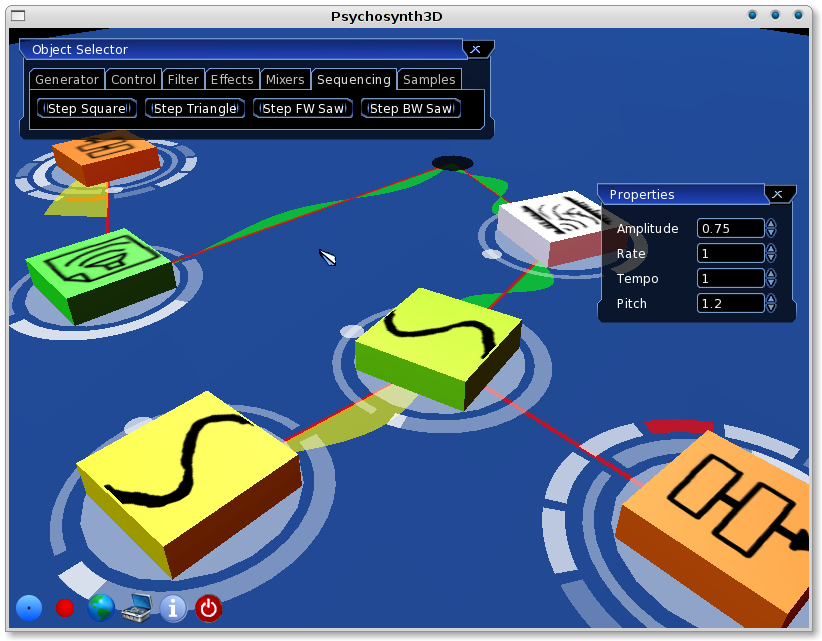
\includegraphics[width=\textwidth]{pic/screenie.png}
  \caption[A screenshot of GNU Psychosynth 0.1.4]{A screenshot of GNU
    Psychosynth 0.1.4.}
  \label{fig:screenie}
\end{figure}

\subsection{A critique on the term framework}

The term \emph{framework} is used many times in this and other
projects and is becoming a techie buzzword. In many contexts it is
abused as a synonym for the term \emph{library}. Instead, we believe
that a framework is something different, following the definition
given in the famous design patterns book by the gang of
four \cite{gamma95design}.

We use the term \emph{library} when the root of the call graph is on
the client side and she invokes the library function sparely to obtain
some concrete functionality. Instead, a \emph{framework} stands in the
root of the call graph and the client code is called through extension
hooks in the framework, following the ``Hollywood principle'' ---
``Don't call us, we'll call you.''.

Because the Psychosynth system is layered, one can just use the bottom
layers as a library, or rely on the upper layers that properly use
inversion of control like a framework.

\subsection{The layered architecture}

At the current stage, GNU Psychosynth implements a layered
architecture \cite{garlan94software}. This intends to promote a more
decoupled design, as calls between modules are only allowed from top
down.

Also, the library has many features, many of which some users may
not need. This layered approach could allow a potential user to avoid
any special overhead when he is only using some bottom layers. Still,
note that the library is now compiled will all layers bundled in the
same shared-object file, so this is not a fact now. Because the heavy
redesign ongoing during this project, we shall postpone that until the
late development stages when the layer interactions are clear and
stable.

Figure \ref{fig:layers} represents the current layered
architecture. Lets make a bit more in-depth discussion of each layer.

\begin{figure}[h!]\centering
\todo{La capa node hay que cambiarlo por \texttt{graph}}
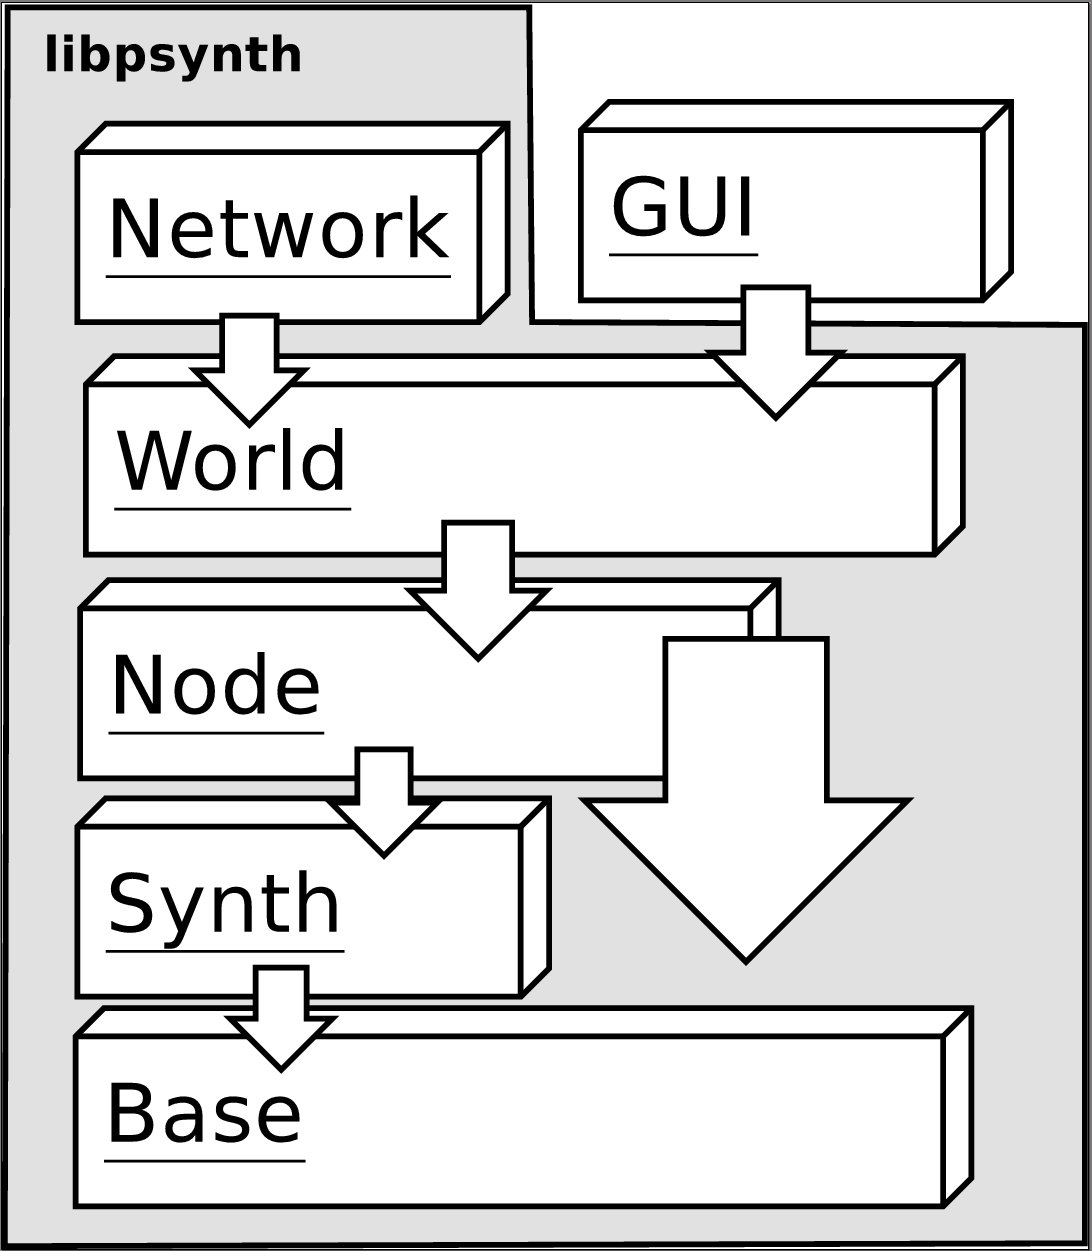
\includegraphics[width=.6\textwidth]{pic/layers.png}
\caption{The Psychosynth layered architecture.}
\label{fig:layers}
\end{figure}

\subsubsection{The \texttt{base} layer}

The base layer includes basic facilities that may be reusable in any
other part of the application. Some of the most relevant examples:

\begin{description}
\item[Configuration persistence] Classes for representing program
  settings in a hierarchical manner. This configuration system can use
  interchangeable backends and has an observable
  interface.\footnote{We use quite often the term \emph{observable
      interface} which is rare in the literature. By this, we mean
    that it provides signals, listeners or other event mechanisms,
    instances of the \emph{observer} design
    pattern\cite{gamma95design}.}

  In fact, we do not recommend using this module in the core of the
  intermediate layers of the library because it can cause unexpected
  coupling, but this is not too clear and we keep it here for
  historical reasons.

\item[Implementation of design patterns] While the term \emph{design
    pattern} means reusable design structure, not reusable code,
  language abstractions can make them implementable as code in some
  cases. Andrei Alexandrescu proves this point for C++ in
  \cite{alexandrescu01modern}. Thus, we provide implementations, quite
  often similar to Alexandrescu's, to various recurring design
  patterns such as \emph{factory} or \emph{singleton}. Some
  implementations are not inspired in Alexandrescu's, like the generic
  \emph{composite}.

\item[Command line argument parsing] While we have considered moving
  to Boost's Program Options library, our own implementation have
  different trade-offs and is rather extensible.

\item[Logging system] A hierarchical and multi backend logging system
  for registering messages from other modules. It should be used
  instead of direct output to \texttt{std::cout/cerr} in all the code.

\item[File management tools] That ease the task of finding resources
  in the hard-drive and can cache results.
\end{description}

Some other minor classes and tools are excluded from this list. During
the development of the project we will drop in this layer classes that
feel interesting at any abstraction level.

\subsubsection{The \texttt{synth} layer}

This layer contains classes for the \emph{static} construction of
synthesisers and sound processing. The audio input and output
facilities are considered to be in this layer, and as well audio
processing data structures ---like ring buffers, multi channel
buffersm, etc.---, basic implementations of filters, oscillators and
audio scalers.

By static, we mean that this code does not provide any dynamic routing
facilities, instead, the programmer is in charge to assign buffers and
call the processing elements manually.

Requisites \ref{req:iter1-begin} to \ref{req:iter1-end} should be
implemented here. Non functional requisites \ref{req:iter1-begin2} to
\ref{req:iter1-end2} are specially relevant in this layer too.

\subsubsection{The \texttt{node} layer}

This layer provides the facilities for the \emph{dynamic} construction
of synthesisers. It includes the mechanisms for describing and
executing the modular synthesis graph with the signal flow and so
on. Figure \ref{fig:node} represents the main concepts behind the
current design. Ports are considered as ``signal ports'' using the
terminology in requirement \ref{req:porttype} --- ``control ports''
are similar to ``parameters'', but parameters are not a precise model
of ``control ports'' as they can not be routed and are intended for
communication between the client user interface code and the audio
thread state.

The communication system used to propagate values between the audio
processing thread and the client thread is represented in figure
\ref{fig:thread}. Values are copied to and from an intermediate channel
between the audio processing blocks. 

\begin{figure}[h]
\centering
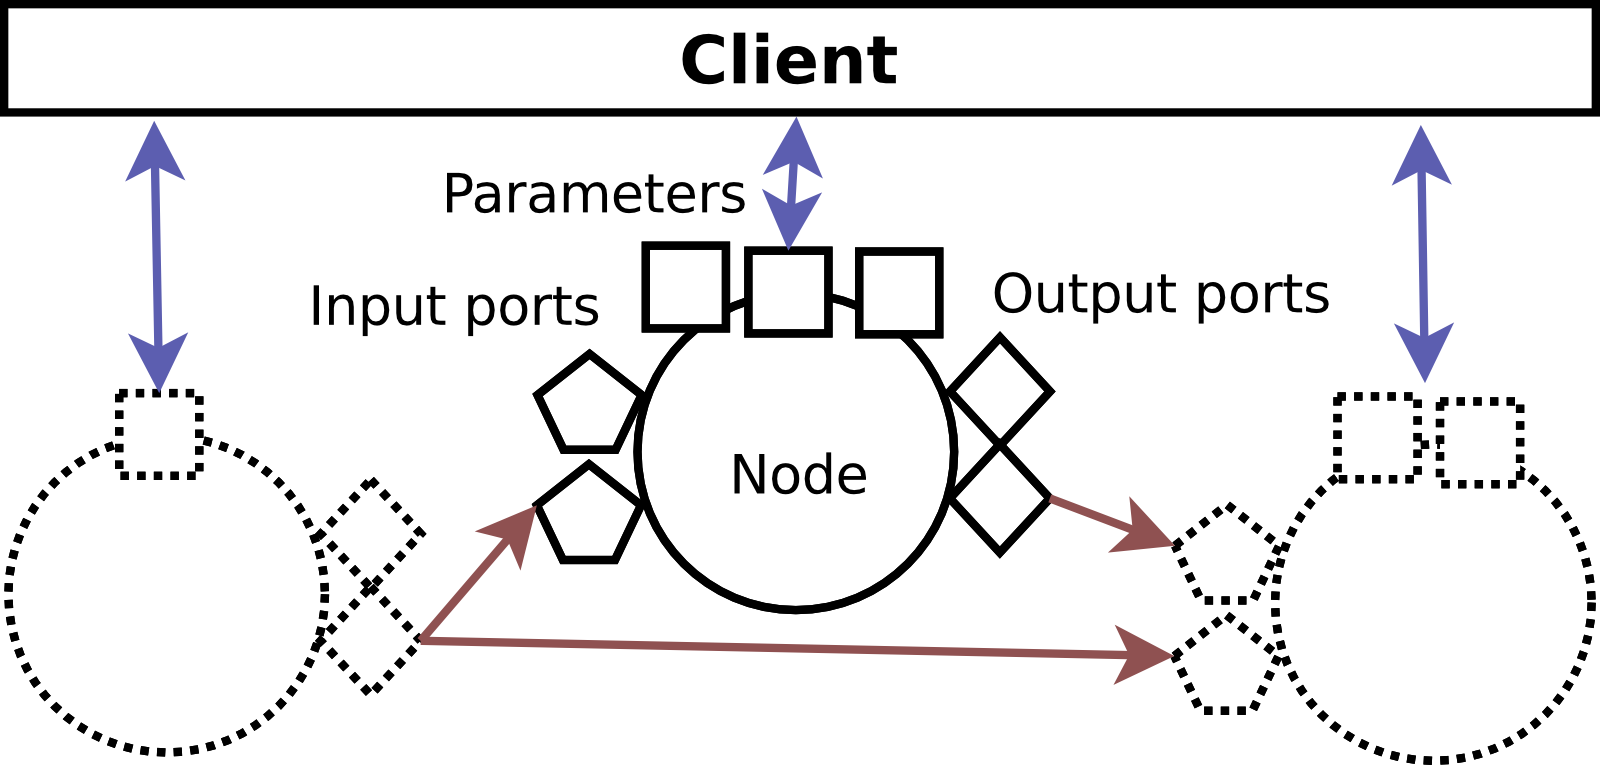
\includegraphics[width=.6\textwidth]{pic/node.png}
\caption[Representation of the node graph as in Psychosynth
0.1.7]{Representation of the node graph as in Psychosynth 0.1.7. Input
ports are represented as pentagons, output ports as rombus and
parameters as squares.}
\label{fig:node}
\end{figure}

\begin{figure}[h]
\centering
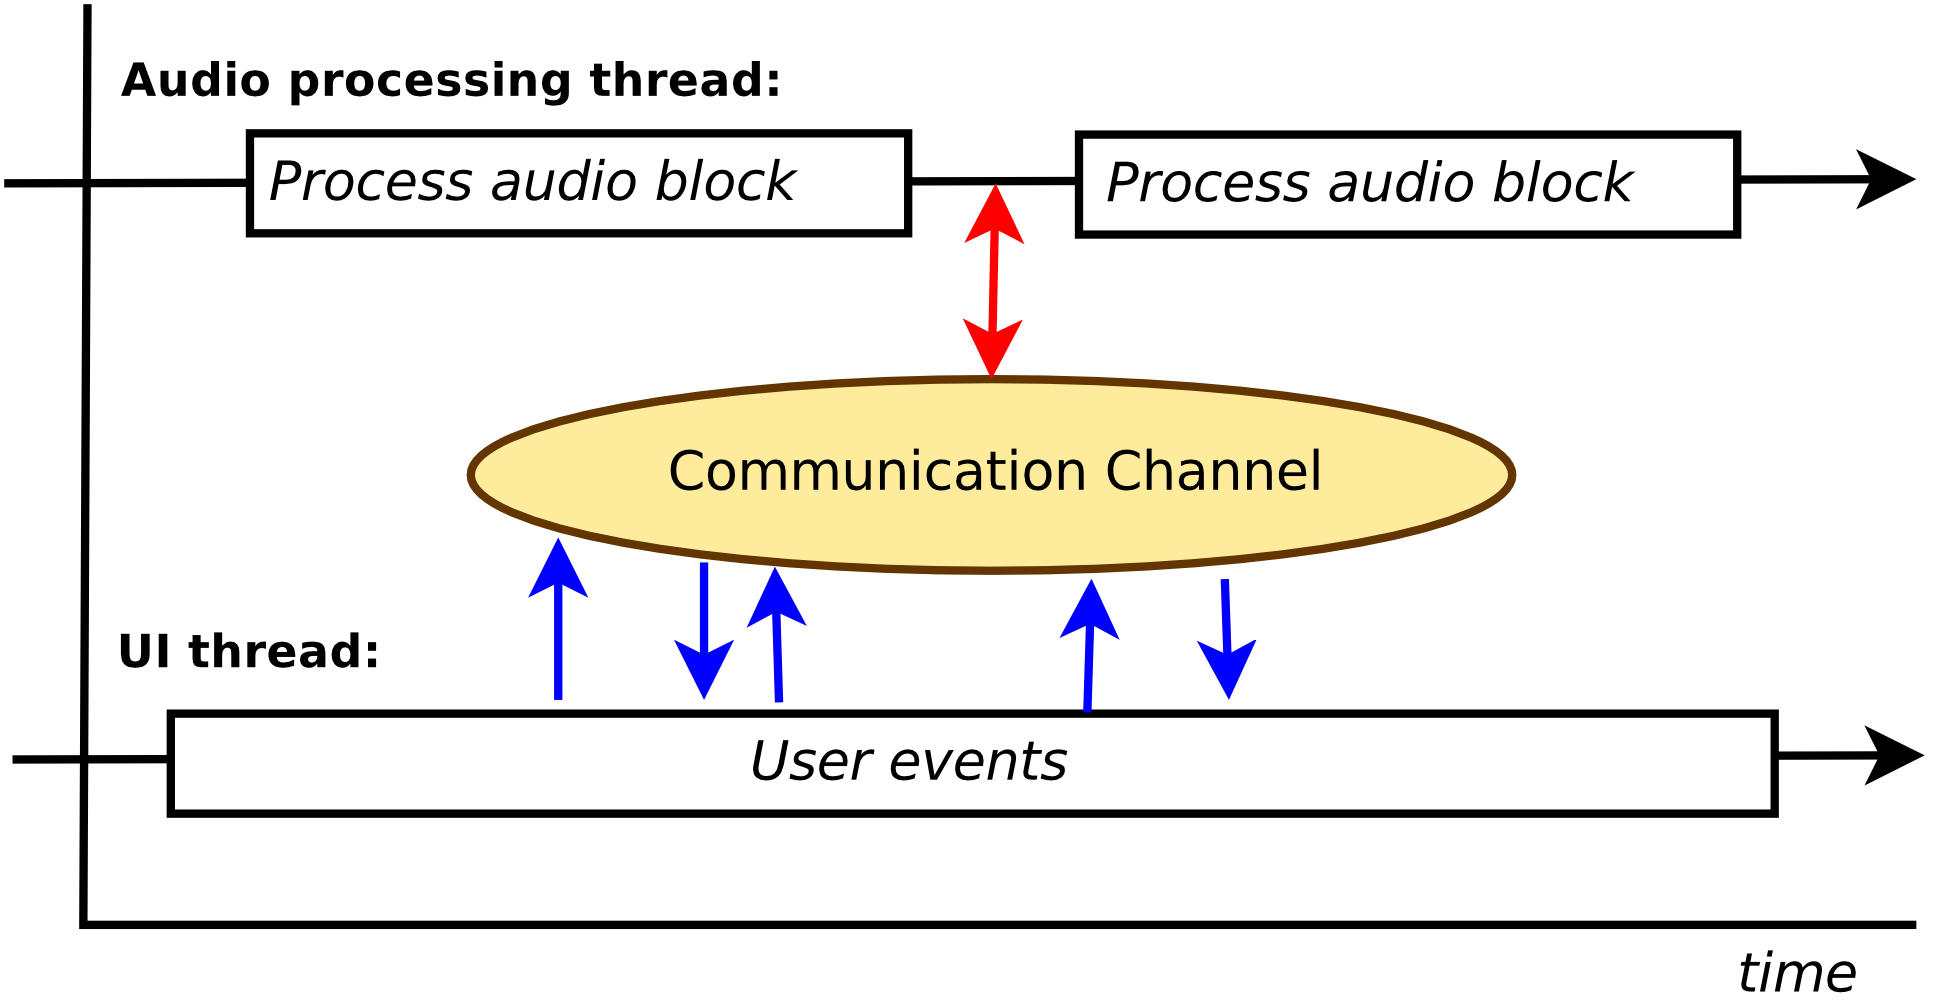
\includegraphics[width=.7\textwidth]{pic/thread.png}
\caption{Communication between the audio and user interface thread as
  in Psychosynth 0.1.7}
\label{fig:thread}
\end{figure}

Requisites \ref{req:iter2-begin} to \ref{req:iter2-end} should be
implemented in this layer. A heavy redesign of its API and many of its
internal implementation is to be expected for that to be accomplished.

\subsubsection{The \texttt{world} layer and the Model View Controller
  architecture}

This layer simplifies the interface exposed to the previous layer and
makes it \emph{observable}. This is fundamental for the Model View
Controller that the system implements.  Figure \ref{fig:mvc}
represents this architectural style. On the following, we can refer to
this observable interface abstracting the synthesis engine as
\emph{the model}.

\begin{figure}[h!] \centering
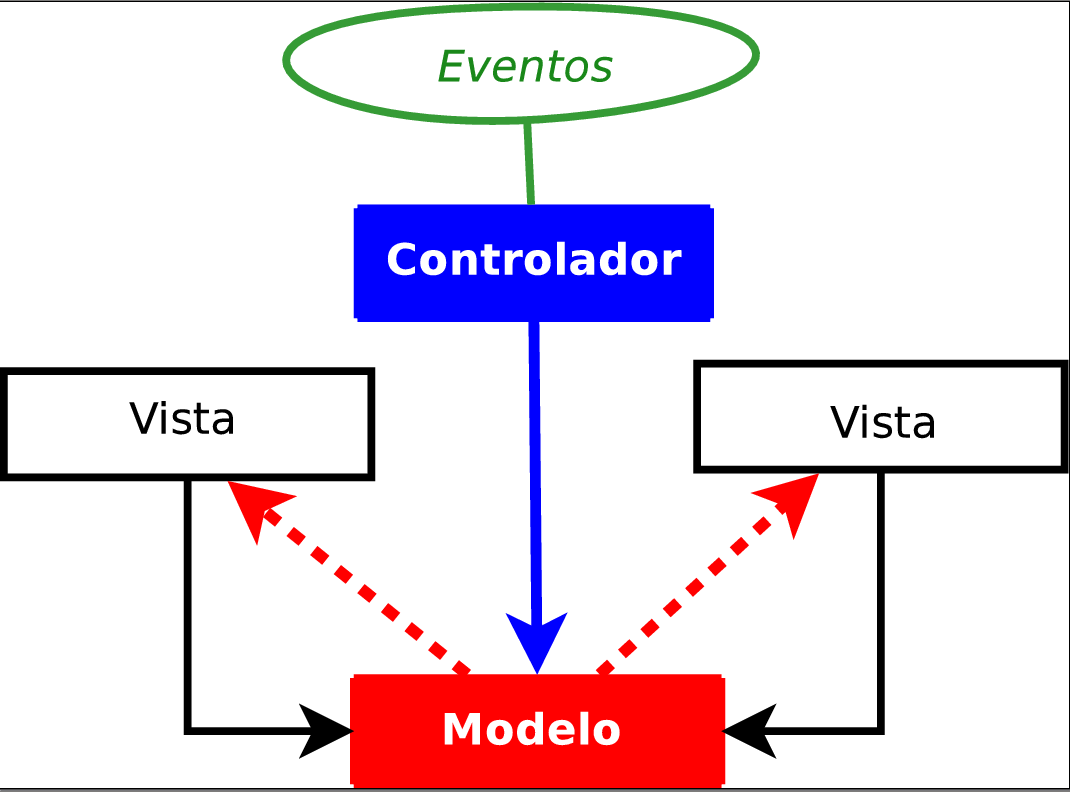
\includegraphics[width=.5\textwidth]{pic/mvc.png}

\todo{Mejorar y traducir esta figura.}

\caption[The MVC architectural style]{The Model View Controller
  arquitectural style. Dashed arrows represent indirect invocation
  ---i.e. via the \emph{observer} design pattern--- and normal lines
  represent normal method calls and data access.}
\label{fig:mvc}
\end{figure}

Several views can coexist independently ---for example, a GUI user
interface and a web client---, that get updated whenever a value has
changed in the model. They register themselves on the model at the
beginning and then become passive entities that get called by the
model. The model changes when controllers invokes methods on it,
several controllers can coexists too. Usually, models and views come
in pairs. For example, a GUI view has an associated controller that
triggers the manipulation of the model in the eventuality of certain
user actions like clicking a button; in this case the representation
(the buttons) and the action (clicking it) are strongly related, but
this is not necessarily true for other situations.

This layer also abstracts the graph interconnection mechanism using
the \emph{strategy} design pattern. Concretely, dynamic patching is
implemented here and the interface exposed in this layer hides the
manual node interconnection mechanisms but provides observability for
topological changes.

This layer should implement requisite \ref{req:views}. 

\subsubsection{The application framework layer and the view and
  controller layers}

There is a thin layer, instance of the \emph{facade} pattern, called
\texttt{app}, that was hidden for simiplicity in figure
\ref{fig:layers} representing the layered architecture. It sits on top
of the \texttt{world} layer and is in charge of initialising the
\emph{world} and defines a configuration tree, using the facilities in
the \texttt{base} layer, and setups the machinery using the
observability of the configuration system to keep coherence between
the user preferences and the status of the synthesis model --- for
example, if the ``\texttt{psynth.output}'' setting is changed, it
automatically creates the appropriate output object instance, sets its
values and substitutes the output node in the synthesis graph. This
layer also sets up the command line argument parsing and installs some
common audio setting arguments in the parser. This layer is where
Psychosynth becomes a framework at its most pure level, as it offers a
\texttt{psynth\_app} class whose \texttt{run} method
should be the only call in the program \texttt{main}, and in turn
delegates the heavy work to user code that is hooked as method
overrides of that same class.

Orthogonal to this layer and sitting also on top of the \texttt{world}
layer the networking layer offers a set of views and
controllers\footnote{A primitive implementation of such at this stage
  of the development.}  that can be used to create the shared
environment described in requirement \ref{req:sharedenv} and thus
allowing collaborative performances. This is an example of the value
of the MVC architecture: because views and controllers are orthogonal,
the user interface does not need to know about the presence of this to
function properly; one could develop a new experimental and cool UI
and it would automagically be able to work with third party clients
over the network, even potentially using a different user interface.

On top of all this there is in the current version of Psychosynth the
code of the 3D user interface and small and simple command line tools
intended to be used as GUI-less network capable clients and
servers. But all this code is not part of the framework, as it wants
to be user interface agnostic, so we will not further describe that
code.

\section{Project planning and methodology}

\subsection{Rationale --- A critique on software engineering}

Choosing a well known software engineering process is considered one
of the first steps to be taken in a final master thesis project. In
our school we study with most detail the Cascade Process and the
Unified Rational Process.

Those development processes propose a fordist software production
model, targeted at huge development teams and the development of
stable code bases in non innovative well defined fields. Martin Fowler
makes a great point \cite{fowler01design} criticising the often
repeated argument stating that software engineering is like any other
engineering where creative analysis and design is only the first step
and thus coding is analogous to construction. As he says, the
construction is done by the compiler and people involved in
programming are actually doing an intellectual and creative work too
--- in computing, any systematic task can and must be automated. The
$programming=construction$ metaphor is alienating for the programmer,
who is completely excluded from the task of criticising and improving
the software design, and thus this metaphor often leads, in the end,
to bad software.

Moreover, fordist development models take risk control and client
requirements satisfaction as most important factors. Because we are in
an academic environment, there are two more important factors: the
pedagogical value of the project ---this is, that the student involved
takes the risk of exploring the unknown by himself--- and the research
value ---this is, that the student involved takes the risk of
exploring the unknown by humanity.

Of course, this is neither a pure research project, so we can not
substitute a software development project by the scientific
method. But we can choose a more dynamic methodology that includes
\emph{falsification} in one way or the other; \emph{agile}
methodologies\footnote{\url{http://agilemanifesto.org/}} propose many
alternatives that could be valid for a master thesis project.

Still, these methodologies are, we believe, inadequate for this
concrete project. The main reason is that this project is developed by
only one person. Most methodologies, specially agile ones, put
emphasis on the developer communication methods and collective
decision making, so they are often inadequate and too constraining and
time consuming for an unipersonal team.  The Personal Software
Proccess \cite{watts96psp} proposes a methodology that is specially
targeted at personal software developed by engineering
students. Sadly, we are not very familiar with it ---and do not have
enough time to make that happen within the time constraints of the
project--- and it seems too be to specific and time consuming in its
time tracking proposal.

Because we still believe that some rational planning and methodology
is needed, we propose in the following a defined but unconstrained
methodology that is specially tailored for our circumstances,
capturing the most common elements in other software processes.

\subsection{An iterative development model}

Because of the size and complexity of the project, we should not
consider developing it all at once. Moreover, the layered architecture
of the starting code base and the variety of requirements that we want
to satisfy favour an iterative development.

For all this, we want to split the development in iterations. Each
iteration is composed by the following phases:  \emph{design},
\emph{implementation}, \emph{verification} and
\emph{integration}. Each iteration shall be assigned a set of
requirements from the specification in section \ref{sec:requirements}
that are to be satisfied after the successful accomplishment of that
iteration.

\subsubsection{The design phase}

In the design phase we shall define the API that we would like the
current subsystem have. Because we are developing a library and
framework with a public interface, the design phase is specially
relevant shall be done with care.

We do not enforce a particular method for documenting the design as
different paradigms favour different documentation means. For example,
in the first iteration we will develop a library heavily based on
metaprogramming, where UML does not fit very naturally. Still, the
documentation should include rationale explaining why the design
decision lead to the satisfaction of the requirements that we want to
satisfy after this development iteration. Also, it may be found that a
requirement may be impossible to satisfy on the current iteration or
that this requirement is to be better integrated in some other
iteration. The developer is free to reassign that requisite for later
iteration properly documenting this as a post-analysis plan fix.

What we do enforce is that all the API is documented with Doxygen for
the sake of completeness of the reference manual that you should
receive along with this document.

\subsubsection{The implementation phase}

During the implementation phase the code implementing the design
should be written. It is possible and even recommended to modify the
design during this phase as inconsistencies and fundamental problems
are found. Sometimes, this may even start as soon as design, specially
when it is unclear the properties that such API should have and some
``exploratory programming'' is needed. This fact may or many not be
documented at the beginning of the section --- even though an API may
be designed through an inductive empirical process, a deductive
rational description may be more useful for its clear understanding.

\subsubsection{The verification phase}

In the verification phase we perform \emph{unit tests} on the most
important parts of the system. No iteration should be considered
finished unless proper unit tests are written and satisfied for its
core components. For writing such tests the Boost Unit Testing
Framework should be used.

When some elements are considered relevant to performance
requirements, \emph{performance tests} should be included. While we do
not enforce a specific performance testing technique here, the
tests should be reproducible and automatable whenever possible.

\subsubsection{The integration phase}

When a subsystem is added and it is to replace an existing subsystem
in the project, the older code should be removed and the layers on top
modified such that they use the new code. This might even be
considered part of the verification, as older tests working on the
upper layers should be checked to be working still.

Informal integration tests should be done on the final user interface
to make sure that the older properties are preserved. Note that in
most cases, we do not recommend to lose time editing the old user
interface such that the new features in the framework are exposed to
the user. Of course, that the new features are usable is the final
objective, but as it was justified in \ref{sec:userinterface}, a
completely new user interface will be developed as part of a future
project.

\subsubsection{Recursive decomposition of iterations}

In practice, some of the expected requirements to be satisfied may be
found orthogonal or maybe too big to be addressed at one. It is thus
allowed to recursively decompose an iteration in sub-iterations when a
first evaluation during the design phase suggests that.

\subsection{A project plan}

\subsubsection{First iteration: A metaprogramming based sound
  processing foundational library}

This iteration is here to deeply re-design the core data structures
using the latest techniques in C++. This requires special research and
performance requirements deeply rely on the success of this
iteration. 

Requirements \ref{req:iter1-begin} to \ref{req:iter1-end} and
\ref{req:iter1-begin2} to \ref{req:iter1-end2} should be satisfied for
its success.

Etimated time cost: 6 weeks.

\subsubsection{Second iteration: Redesign of the \texttt{node} layer
  for hierarchy and polyphony}

The \texttt{node} layer requires a redesign if we want to satisfy all
our purposes. Polyphony and hierarchy would be specially tricky to
implement directly on top of the current code base. A special
evaluation of how the new design interacts with the MVC architecture
and networking is required. The \texttt{world} layer may be affected
too. All the design changes should be implemented too.

Requirements \ref{req:iter2-begin} to \ref{req:iter2-end} should be
satisfied for its success. Requirement \ref{req:persistence} may be
considered for its implementation in this iteration too.

Estimated time cost: 6 weeks.

\subsubsection{Third iteration: Dynamic loading of nodes}

In this iteration the plugin system is to be developed.

Requirements \ref{req:iter3-begin} to \ref{req:iter3-end} should be
satisfied for its success.

Estimated time cost: 4 weeks.

\subsubsection{Fourth iteration: Adding MIDI and synchronisation}

Synchronisation and MIDI support is one of the most important
features and it is also one of the features we know the least about,
thus, we should put special care on research and design. This will
affect the node and world layers mostly.

Requirements \ref{req:iter4-begin} to \ref{req:iter4-end} should be
satisfied for its success.

Estimated time cost: 8 weeks.

\subsubsection{Post mortem analysis}

After the conclusion of all the previous iterations, we should write a
conclusive report and evaluation of its success. Also, we should
prepare a final presentation for its evaluation.

%%% Local Variables: 
%%% mode: latex
%%% TeX-master: "00-main"
%%% End: 


\chapter{A generic sound processing library}

\epigraph{Numbers it is. All music when you come to think.  Two
  multiplied by two divided by half is twice one.  Vibrations: chords
  those are. One plus two plus six is seven. Do anything you like with
  figures juggling. Always find out this equal to that. Symmetry under
  a cemetery wall. He doesn’t see my mourning. Callous: all for his
  own gut. Musemathematics. And you think you’re listening to the
  etherial. But suppose you said it like: Martha, seven times nine
  minus $x$ is thirtyfive thousand.  Fall quite flat. It’s on account of
  the sounds it is.}{\emph{Ulysses}\\\textsc{James Joyce}}

\section{Analysis}

Requirements \ref{req:iter1-begin} to \ref{req:iter1-end} and
\ref{req:iter1-begin2} to \ref{req:iter1-end2} refer to the second
layer of our system --- in a bottom-up approach. The most crucial
question here: how do we represent a sound in a computer? Then, a new
question arises: how do we get the sound to the speakers? The later
question has a trivial answer --- use whatever API your operating
system exposes for delivering sound to the soundcard --- but the first
question is still to be answered. Actually, the solution to this first
question mostly subsumes the issue of how to interface with these
external interfaces, thus, shall we debate it with care.

\subsection{Factors of sound representation}
\todo{Me he dado cuenta de que esta sección introduce muchas
  definiciones. ¿Tal vez utilizar un estilo más formal usando el
  paquete theorem para las definiciones ayudaría a usar el documento
  como referencia?}

A sound signal is a longitudinal wave of air in motion. We can
analogically record the \emph{proximal stimuli} --- i.e. the physical
stimuli leading to the subjective act of perception
\cite{goldstein01sensation} --- sound by measuring the successive
oscillating values of air pressure in the observer's point in
space. Note that an static air pressure value can not be perceived and
the sensation of sound is caused by the relative oscillation of this
measure. The \emph{amplitude} of this change is associated to our
perception of \emph{loudness}, the frequency of this oscillation
mostly logarithmically determines our perception of pitch. We phrased
this conditionally because these two variables are actually
interrelated and our actual subjective perception of loudness might
vary with pitch and otherwise \cite{fletcher37loudness}.

Most of the time, we represent the relative air pressure value as a
voltage, that varies at some range --- p.e. $[ -5, 5 ] V$. This is an
analogous signal that we have to discretise somehow in order to
manipulate it computationally.

\subsubsection{Temporal quantisation}

Temporal quantisation relates to how many times per second do we store
the current voltage or air pressure value. The value of the signal
between to equally spaced in time samples is unknown, but we can use
some interpolation method to \emph{upsample} a signal --- i.e. to
figure out what is between two samples. Most of the time we refer to
the \emph{sampling rate}, in hertz, as the frequency of the temporal
quantisation.

We know from \emph{Niquist-Shannon sampling theorem} that perfect
reconstruction of a signal is possible when the sampling frequency is
greater than twice the maximum frequency of the signal being sampled,
or equivalently, when the \emph{Nyquist frequency} (half the sample
rate) exceeds the highest frequency of the signal being
sampled. Because the hearing range in most human beings is 20 Hz--20
kHz, audio compact discs use a 44.1 kHz sampling rate. Other popular
rates in audio production are 48 kHz, 96 kHz and 192 kHz. Sampling
rates bellow 44.1 kHz are used also in old computer games that were
limited by the computing power and low bandwidth systems such as
telephone, where low cost and proper understanding of human speech is
more important than audio fidelity.

The sound representation mechanism itself does not vary with the
sampling rate, and thus supporting various rates depends more on the
implementation of the signal processing units and the overall
performance of the system, with the CPU being able to process so many
samples per second being the biggest constraint.

\subsubsection{Spatial quantisation}

Spatial quantisation determines how many possible values can a sample
take in our finite and discrete scale. In a computer system, this is
determined by the size in bits of the underlying type used to store
the samples. An audio CD uses a \emph{bitdepth} of 16 bit with samples
that can take $65.536$ possible values while professional audio uses 24
bit or 32 bit samples. We can even see systems using 64 bit samples
during the processing to avoid accumulative rounding problems due to
heavy arithmetic. The \emph{dynamic range} of a signal with $Q$-bits
quantisation is:
\begin{equation}
  \mathrm{DR_{ADC}} = 20 \times \log_{10}(2^Q) = (6.02 \cdot Q)\, \mathrm{dB}
\end{equation}
The maximum \emph{signal-to-noise} ratio for such a system is:
\begin{equation}
  \mathrm{SNR_{ADC}} =  \left (1.76 + 6.02 \cdot Q \right )\ \mathrm{dB}
\end{equation}

Most analog systems are said to have a dynamic range of around 80 dB
\cite{fries05digital}. Digital audio CD have a theoretical
dynamic range of 96 db --- actual value is around 90 db due to
processing. Human hearing pain level is at 135 db but actually
prolonged exposure to such loud sound can cause damage. A loud rock
concert is around 120 dB and a classical music performance is at
110 db \cite{ludwig09music}, thus requiring bitdepth of at least 24
bit (theoretical dynamic range of 144 dB) for perfect fidelity.

There are some other aspects related to representation of samples in a
computer, such as the \emph{signedness} of the underlying type. Signed
types are usually considered more convenient for audio signals as 0
can be easily recognised as the still no-sound value simplifying
computations. Another important factor is whether we use \emph{fixed
  point} or \emph{floating point} arithmetic. While fixed point is
used in low-cost DSP hardware, floating point is the most common
representation in current audio software as nowadays processors are
optimised for SIMD\footnote{Single Instruction Multimple Data, as
  supported by MMX, 3D Now! and SSE extensions in Intel and AMD chips}
floating point arithmetic. Moreover, the algorithms implementation is
much harder to encode because products produce greater values and
there are many ways on how to account the carry.  Actually, even while
the actual bitdepth (the bit for the mantissa) of a 32 bit floating
point is the same of a 24 bit fixed point, then a 32 bit fixed point
will have a quite lower \emph{quantization error}, but the dynamic
range and SNR of a floating point is much higher because the
values are spaced logarithmically over a huge range
\cite{smith02dsp}. Another factor is the \emph{endianess} of fixed
point values but is relevant only when interfacing with file formats
and output devices.

\subsubsection{Channel space}

Because our hearing system is dicotomically symmetric, audio
engineers discovered that much better fidelity can be achieved by
reproducing the sound with some differences from two separate
loudspeakers. This is the well-known \emph{stereophonic} sound,
commonly named just \emph{stereo}.

For representing such a signal, two different streams of information
are needed for the left and right channels. Moreover, nowdays
\emph{quadraphonic}, and \emph{surround} sound with varying numbers of
channels up to 20.2 are used in different systems.

We call \emph{channel space} to the set of semantic channels we use in
some sort of audio representation --- p.e. stereo audio has channel
space with $left$ and $right$ elements. We use the term
\emph{frame} to call a set of samples coincident in time, this is, the
samples of the various channels at a given time point. Thus, we will
use most of the time the more accurate term \emph{frame rate}.

This rises the problem on how to linearise the multi channel data. The
most common mechanism in domestic hardware is by \emph{interleaving}
the samples of different channels, this is, by storing the frames
sequentially. However, high-end hardware often accepts data in
non-interleaved form where the samples of each channel is stored in a
separate sequence. In this document, we borrow from the image
processing world the term \emph{planar} to refer to non-interleaved
data. Software doing a lot of processing of the audio signal often
chooses this representation as it is easier to scale to varying number
of channels and split the signal to do per-channel filtering. Figure
\ref{fig:interleaving} compares visually the interleaved and planar
formats.

\begin{figure}[h]
  \centering
  \subfloat[]{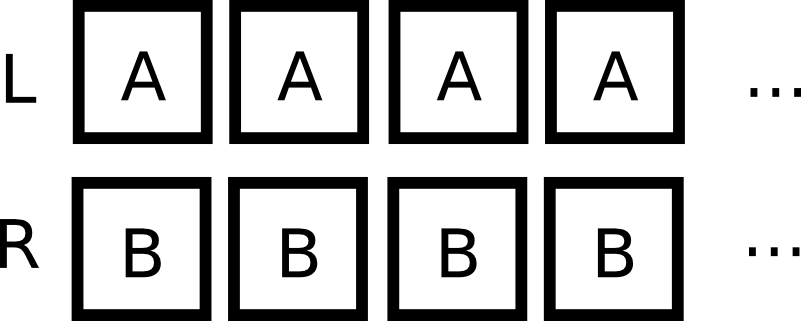
\includegraphics[width=2in]{pic/fmt-planar.png}}\;
  \subfloat[]{
\includegraphics[width=3in]{pic/fmt-interleaved.png}}
  \caption{Multi-channal data in planar (a) and interleaved (b) form.}
  \label{fig:interleaving}
\end{figure}

Another issue is the order in which the data from different semantic
channels is stored. We call a \emph{channel layout} a bijection $L : C
\rightarrow \mathbb{Z}_{\|C\|}$, where $C$ is a given \emph{channel
  space}. For example, the mapping $\{ left
\mapsto 0, right \mapsto 1 \}$ is a common layout for stereo sound,
but $\{ left \mapsto 1, right \mapsto 0 \}$ is sometimes used too.

\subsection{Common solutions}

As we have already noticed, 32 bit floating point sound with planar
left-right layout the most common in software of our kind during
internal processing. As most of this software is written in C, a
simple \texttt{float**} does the job. This was, actually, the internal
representation used in GNU Psychosynth in versions prior to 0.2.0,
wrapped in the \texttt{audio\_buffer} class.

However, this design starts to wobble whenever one has to interface
with some other library or hardware using a different format. Thus,
the \texttt{audio\_buffer} class provided different
\texttt{interleave\_*} and \texttt{deinterleave\_*}, where the
asterisk can be substituted by different sample formats like
\texttt{s16} or \texttt{s32} (fixed point signed 16 bit and 32 bit
respectively). This is very inconvenient because, as we have seen
through this section, many orthogonal factor affect audio
representation inducing a combinatorial explosion of format conversion
functions. Take a look at the 64 different read and write functions in
the \texttt{pcm.c} file of the
LibSndfile\footnote{\url{http://www.mega-nerd.com/libsndfile/}}
library.

This is a maintenance hell, but using the common means for abstracting
orthogonal behaviour variability, i.e. dynamic polymorphism, is simply
not an option in any audio software which supports real-time operation.

\subsection{A generic approach: Boost.GIL}

However, there is a piece of software that proved that this issue can be
solved in C++ using static polymorphism. This is the Generic
Image Library\footnote{http://stlab.adobe.com/gil} which was developed
by Ludovic Cortés et. Al inside Adobe Software Technology Lab that was
later include inside the Boost library distribution.

While sound and image manipulation are quite different, specially from
the psycho-perceptive point of view, they are both a signal processing
problem and thus share a lot in the representational issue. By
realising of a proper conceptual mapping between both worlds (table
\ref{tab:gilmap}), most of the library design and even quite a lot of
code of Boost.GIL can be reused to build a unique state-of-the-art
sound processing library that addresses the aforementioned issues in
an orthogonal generic manner while maintaining near-optimal
performance.

\begin{table}[h]
  \centering
  \begin{tabular}{c|c}
    Boost.GIL & Psynth.Sound \\ \hline\hline
    Channel   & Sample \\
    Color     & Channel \\
    Color Space & Channel Space \\
    Color Layout & Channel Layout \\
    Pixel & Frame \\
    View & Range \\
    Image & Buffer
  \end{tabular}
  \caption{Terminology map from \texttt{boost::gil} to \texttt{psynth::sound}}
  \label{tab:gilmap}
\end{table}

An \emph{image} is bidimensional matrix of \emph{pixels}, that capture
the properties of light electromagnetic waveform at those discrete
points. Each pixel, however, is decomposed in several \emph{colors}
that, for example, capture the intensity in the red, green and blue
sensors of a CCD camera. As there are different ways of decomposing an
audio frame (p.e, stereo, surround, etc.), there are different ways of
decomposing a pixel into several values, known as the \emph{color
  space} (p.e, RGB, CMYK, YUV, etc.). Boost.GIL uses the term
\emph{channel} to name the individual value of one those color
components.

In our audio framework, a \emph{buffer} is unidimensional array of
\emph{frames} that represent a sound or part of a sound --- sound is
continuous and thus we usually process it in chunks. The reader might
note that the the data in a buffer being arranged along the
\emph{time} dimension while the dimensions of an image represent
\emph{physical space} makes these entities completely different from
the processing point of view. However, they share most representation
problems, with sound representation being actually a sub-problem of
image representation, as we have one dimension less. The samples in a
series of audio frames can be stored in an interleaved or planar
fashion as happens with the channels of a pixel. Also, both channels
and samples can vary in signedness, fixed/floating point, bitdepth,
etc.

Those already familiar with Boost.GIL can thus already understand
easily our Psynth.Sound module design and implementation that we are
to describe in the following section.

\section{Design}

\subsection{Core techniques}

The Boost.GIL and thus the Psynth.Sound modules design makes heavy use
of static polymorphism and generic programming via C++ templates to
achieve generality without runtime overhead. We are going to introduce
advanced techniques used in generic programming for the reader
unfamiliar with this programming paradigm.

\subsubsection{Concepts}
\label{sec:concepts}.

\emph{Concepts} \cite{jarvi10concept} are to generic programming what
\emph{interfaces} --- pure abstract classes in C++ --- are to object
oriented programming: they specify the requirements on some
type. However there, are few substantial differences. (1) While
interfaces can only specify the method signatures of its instances, a
concept can specify most syntactic constraints on a type, like the
existence of free functions, operators, nested types, etc. (2) While
dispatching through interfaces requires, at least, a dereference,
addition and function call \cite{driesen96direct}, when using concepts
the concrete function to be executed can be determined and even
inlined at compile-time. (3) One can not declare that a type satisfies
an interface separately from the type definition, but one can say that
a type models a concept at any point of the program. (4) Thus, no
primitive type defines any virtual interface, but one can turn any
primitive type into an instance of any concept via a
\texttt{concept\_map}. (5) Actually, the syntactic properties defined
by a concept its models may differ, but they are matched via the
\texttt{concept\_map}. In fact, C++ concepts are more similar to
Haskell \emph{type classes}, with \texttt{instace} doing the job of
\texttt{concept\_map} \cite{bernardy08comparison}.

Concepts are an extension to the template mechanism to add type
checking for it. In fact, checking and dispatching on requirements can
be achieved with techniques like SFINAE (Substitution Failure Is Not
an Error) \cite{vandervoorde08templates}. Property (5) of our concepts
can be simulated with \emph{traits} \cite{c++traits}. However, both
compiler errors and the code using templates without concepts is
usually much more unreadable.

The proposal of adding concepts to the C++ language was rejected last
year by the standardisation committee and thus we can not use them in
our code. However, Boost.GIL is very influeced by Alexander Stepanov's
deductive approach to computer programming using generic programming
and modeling with concepts, that he elegantly describes in his
master-piece ``Elements of Programming''
\cite{stepanov09elements}. Actually Stepanov worked several years in
Adobe where he held a course ``Foundations of Programming'' based on
his book. Thus, the \emph{modeling} of the library extensively uses
concepts. Its implementation uses a limited form of concept checking
via the Boost.ConceptCheck\footnote{
  \url{http://www.boost.org/doc/libs/release/libs/concept_check/concept_check.htm}}
\cite{siek00concept} library, however, enabling this library in
release mode can affect performance and its syntax is quite more
cumbersome than the concepts in the C++ standard proposal. For
consistency with the Boost.GIL documentation we will use the concept
syntax proposed in the proposal N2081 to the standardisation committee
\cite{gregor06concept}.

The following example defines a concept that is satisfied by every
type that has an \texttt{operator<}:

\begin{lstlisting}
concept LessThanComparable<typename T> {
  bool operator< (T, T);
};
\end{lstlisting}

This allows us to write a generic function that depends on the
existence of a less-than comparator for the parametrised type:

\begin{lstlisting}
template<LessThanComparable T>
const T& min (const T& x, const T& y) {
  return x < y? x : y;
}
\end{lstlisting}

An alternative syntax for specifying that \texttt{T} must satisify the
\texttt{LessThanComparable} concept is the \texttt{where} clause:

\begin{lstlisting}
template<typename T>
    where LessThanComparable<T>
const T& min (const T& x, const T& y) ...
\end{lstlisting}

In fact, this is the only valid syntax when the concept affects
multiple types. Also, the \texttt{where} clause can be used inside
concept definitions to provide specialisation.

Specifying that a type models a concept is done with the
\texttt{concept\_map} device. If the type naturally models the
concept, we can just use:

\begin{lstlisting}
concept_map LessThanComparable<int> {}
\end{lstlisting}

Note that these trivial concept mappings can be avoided by using the
\texttt{auto} keyword in front of the \texttt{concept} keyword in the
concept definition. However, it might happen that a type requires some
wrapping to satisfy the concept. We can do this in the concept map
definition itself.

\begin{lstlisting}
concept_map LessThanComparable<char*> {
  bool operator< (char* a, char* b) {
    return strcmp (a, b) < 0;
  }
}
\end{lstlisting}

Note that this last piece of code is an example of a bad usage of
concept maps, as this specialises the mapping for pointers changing
the expected semantics.

This should suffice as an introduction to concepts in order to
understand the concept definitions that we will later show when
modelling our system. A more detailed view can be read in the cited
bibliography, with \cite{jarvi10concept} being the most updated and
useful from a programmer point of view.

\subsubsection{Metaprogramming}

The C++ template system is Turing complete
\cite{veldhuizen03templates}, thus it can be used to perform any
computation at \emph{compile time}. This was first noted in 1994 by
Erwin Unruh who, in the middle of a C++ standardisation committee,
wrote a template meta-program that outputted the first $N$ prime
numbers on the console using compiler errors \cite{unruh94prime}. Even
though this might seem just a crazy puzzle game, it can be used in
practise and actually new Boost libraries use it extensively. A very
gentle introduction to template metaprogramming can be found in
\cite{alexandrescu01modern}, where Alexandrescu uses them to
instantiate design patterns as generic C++ libraries. A deeper
reference is Abraham's \cite{abrahams04meta}, which focuses on the
Boost Metaprogramming Library\footnote{The Boost.MPL:
  www.boost.org/doc/libs/release/libs/mpl} and introduces the usage of
metaprogramming for building Embedded Domain Specific Languages (EDSL)
in C++. This Boost.MPL, providing reusable meta data structures and
algorithms, is the de-facto standard library for template
metaprogramming\footnote{It is often called ``the STL of template
  metaprogramming''.} and we will use it in our implementation.

Template metaprogramming is possible thanks to \emph{partial template
  specialisation}, that allows giving an alternate definition for a
pattern matched subset of its possible parameter values. A
\emph{metafunction} is thus just a template \texttt{class} or
\texttt{struct} with a public member that holds the result of the
function. It is up to the programmer to choose the naming convention
for the result members of the metafunctions, in the following, we will
use Abraham's style calling \texttt{type} for result values that are a
type, and \texttt{value} for integral values. Listing \ref{lst:fib}
illustrates how can we write and use a metafunction for computing the
$n$-th Fibonacci number.

\begin{lstlisting}[float=h!, 
  caption=Metaprogram for computing the Nth Fibonacci number,
  label=lst:fib]
template <int N>
struct fib {
  enum { 
    value = fib<N-1>::value + fib<N-2>::value; 
  };
};

template <>
struct fib <0> {
  enum { value = 0 };
};

template <>
struct fib <1> {
  enum { value = 1 };
};

int main () {
  return fib<42>::value;
}  
\end{lstlisting}

The program returns the forty-second Fibonacci value. However, it will
take no time to execute, because the number is computed at compile
time. We use recursion to define the metafunction for the general case
and the specialise for the base cases.

If we consider the template system as a meta-language on its own, we
should describe its most outstanding semantic properties. It is a pure
functional programming language, because variables are immutable. It
is lexically scoped. It supports both lazy and strict evaluation,
depending on whether we choose to access the nested \texttt{type}
result name at call site or value usage type. When we look at the meta
type system, we find three meta types: types (which are duck-typed
records), integrals (e.g. \texttt{int}, \texttt{char}, \texttt{bool}
...) and meta-functions (i.e. templates).

The fact that records are duck typed but integrals and metafunctions
cause several inconveniences in practice, specially when dealing with
the later. For example, in the absence of template aliases, returning
a metafunction produced by another function requires defining a nested
struct that inherits from the actual synthesised value. Also, the
template signature should be specified on a template parameter
expecting a template.

In order to simplify our meta type system we shall wrap constants in a
type like on listing \ref{lst:integral_c}.

\begin{lstlisting}[float, 
  caption=Integral constant nullary metafunction  wrapper.,
  label=lst:integral_c]
template <typename T, T V>
struct integral_c
{
  BOOST_STATIC_CONSTANT(T, value = V);
  typedef integral_c<T, V> type;
};
\end{lstlisting}

There are a couple of issues regarding this definition worth
explaining. First, the \texttt{BOOST\_STATIC\_CONSTANT} macro is used
to define a constant. Internally, it will try to use \texttt{enum} or
any other mechanism available to actually define the constant such
that the compiler is not tempted to allocate static memory for the
constant. Second, the \texttt{typedef} referring to itself turns a
constant value into a self returning nullary meta-function. This can
be very convenient because, for example, it allows using
\emph{value}\texttt{::type::value} always on the value usage point,
allowing the caller or producer of the value to choose whether he
wants to evaluate the value lazily.

Because we just wrapped values into a type, we can simplify our
conventional definition of \emph{metafunction}: a meta-function is any
type --- template or not --- that has a nested type called
\texttt{type}.

Now we should also turn metafunctions into first class entities of the
meta-language. We just add a new level of indirection and define a
\emph{metafunction class} as a type with a nested template
metafunction called \texttt{apply}. The example in listing
\ref{lst:high_order_fib} also illustrates the metafunction forwarding
technique when defining the nested \texttt{apply} metafunction by
inheriting from \texttt{fib}.

\begin{lstlisting}[float, caption=Metafunction class for
  computing Fibonacci numbers. We suppose that the previous
  \texttt{fib} definition uses \texttt{integral\_c} to wrap its
  parameters and return types., label=lst:high_order_fib]
struct fib_class { 
   template <class N>
   struct apply : public fib<N> {};
};

int maint ()
{
  return fib_class::apply<integral_c<int, 42>>
           ::type::value;
}
\end{lstlisting}

Using this convention the MPL library defines many useful high order
metafunctions that take metafunction classes as input, like
\texttt{mpl::fold} and \texttt{mpl::transform}. Note that it is not
needed to define metafunction classes for all our metafunctions,
instead, we shall convert them when needed using the
\texttt{mpl::quote}\emph{N} functions and the \texttt{mpl::lambda}
facility.

\subsection{Core concepts}

We are now ready to understand the main design and implementation
techniques used in our generic library. Because the library is
\emph{generic}, in the sense of generic programming, most algorithms
and data structures are parametrised such that they can be
instantiated with any concrete type modelling some concepts as we
suggested in section \ref{sec:concepts}. Thus, traditional modelling
techniques like the Unified Modelling Language are not useful since
they are intended for object oriented design.

We are going to follow the following methodology for describing the
library. First, we will name a concept and give a brief description of
its purpose. Then, we will define the concept using the notation
described in section \ref{sec:concepts} and finally we will enumerate
and describe some models for such concept.

For brevity, we will omit basic concepts such as
\texttt{CopyConstructible}, \texttt{Regular}, \texttt{Metafunction},
etc. Their complete definition should be evident and an interested
reader can find most of them in \cite{stepanov09elements}.

\subsubsection{\texttt{ChannelSpaceConcept}}

A channel space is a sequence of whose elements channel tags (empty
types giving a name )

\begin{lstlisting}
concept ChannelSpaceConcept<
           MPLRandomAccessSequence Cs> 
{};
\end{lstlisting}

Some example models include \texttt{stereo\_space} or
\texttt{surround\_space}. An example on how a user of the library can
define his own channel space follows.

\begin{lstlisting}
struct left_channel;
struct right_channel;

typedef mpl::vector<left_channel, right_channel> 
        stereo_space;
\end{lstlisting}


\section{Validation}


%%% Local Variables: 
%%% mode: latex
%%% TeX-master: "00-main"
%%% End: 


\chapter{A modular synthesis engine}

\epigraph{We can now see that the whole becomes not merely more, but
  very different from the sum of its parts.}{\emph{More is Different:
  Broken Symmetry and the Nature of the Hierarchical Structure of
  Science}\\\textsc{Philip Warren Anderson}}

\section{Analysis}

In the previous chapter we built a system for sound representation,
processing, and interfacing. In such system, interactions
between different processing elements is hard-coded in the control
flow of the program itself and the relations among the statically
parametrised types that intervene.

As described by requirements \ref{req:iter2-begin} to
\ref{req:iter2-end}, we shall develop a system where the basic DSP
units can be composed orthogonally and hierarchically to build complex
devices \emph{at runtime}. With the applications built on top of our
framework being targeted at live performances, it should be
particularly dynamic.

\subsection{An abstract model of a modular synthesiser}

In a modular synthesiser, the sound generation is made by
interconnecting basic processing units. Each of them might generate
sound, filter it, and can have a varying number of inputs and outputs
of different kinds. Because a module can apply virtually any
mathematical function to its inputs; we can realise any synthesis
technique --- i.e. additive, subtractive, FM/PM --- by just wiring the
available modules in an appropriate way.

We can characterise such a system by abstracting the parts of one of
these processing units. A hardware modular synthesiser can be used to
illustrate the concepts behind this, as shown by the \emph{frequency
  shifter}\footnote{A frequency shifter is a module that produces
  oscillating modifications on the frequency components of a given
  input signals, producing interesting Doppler effects, binaural
  effects, vibratos, and so on.} in figure \ref{fig:hwmod}. We can thus
taxonomise its parts as in the following; we will later use this
terminology in our design.

\begin{description}
\item[Input ports] These are the signals that come from another module. In
  the example figure we can see a \emph{input} signal that carries an
  arbitrary sound wave to be frequency-shifted, and a \emph{CV in},
  which is used to modulate the shift parameter. In a hardware module
  we can consider as an input anything that can go through a wire,
  thus we are no limited just to analog time-domain signals, but we
  can consider a digital MIDI input of a synthesiser as an input
  signal too.

  In our software system we are even less constrained, and our system
  should cope with signals of any kind --- i.e. of any type, in the
  programming language sense. Note also that an input might remain
  disconnected during execution of the synthesis graph, and a proper
  default behaviour should be implemented in that case.

\item[Output ports] These are the signals that the module sends to other
  modules. They are of the same nature than their input counterparts.

  In order to connect an output to an input, the kind of signals that
  flows through them must match; in a computer based digital system
  this should be checked and proper error handling must come into
  action if necessary or maybe some automatic conversion mechanism if
  safe and applicable.

  Note that while on and hardware synth inputs and outputs are
  generally related in a one-to-one manner --- unless we do not
  consider a hub/split or a mixer a module by itself but a connection
  device --- in software we can relate them in a one-to-many fashion,
  as the value produced in an \emph{output port} can be read several
  times by different modules if it has its own memory.

\item[Parameter controls] These allow the user to tune the different
  settings of the device. In a hardware device, they are most of the
  time represented by a knob or a slider, but modern synthesisers
  include bidimensional touchpads and other input devices for
  controlling the process.

  Note that, at this stage, the notion of a \emph{parameter} or
  \emph{control} is not directly related to how it might be
  represented to the user --- like a text-box, virtual knob, or
  whatosever --- but to the abstractions that the a DSP module uses to
  get input from outside of its inner processing function. Just like
  an input port, it should be of any type. For example, any control
  that is naturally representable with a knob or slide is quite often
  a \emph{float} parameter.

  The reader might wonder how is this different from an input port in
  a software system. On the one hand, controls do not have any
  built-in interconnection system. On the other hand, the
  synchronisation mechanisms used to pass the values through controls
  and ports are quite different. This is so because while the
  information that goes through ports is to be used only by the DSP
  modules, controls get input from the user interface thread, thus
  requiring special care. We will discuss this further in the next
  section.

\item[Status controls] These provide feedback to the user about
  relevant parts of the state of the processing. In the example
  figure, a red led is light up when the output signal exceeds the
  \emph{clipping value} --- i.e. the upper threshold of the admissible
  range of the amplitude of the signal --- suggesting the user to
  lower the gain to avoid annoying distortion. Everything that have
  been said about parameter control applies here. Once again, what is
  important is the abstraction not the visual representation; those
  the aforementioned example would be a \emph{boolean} status control in our
  system, that might be represented by any other means.
\end{description}

\begin{figure}
  \centering
  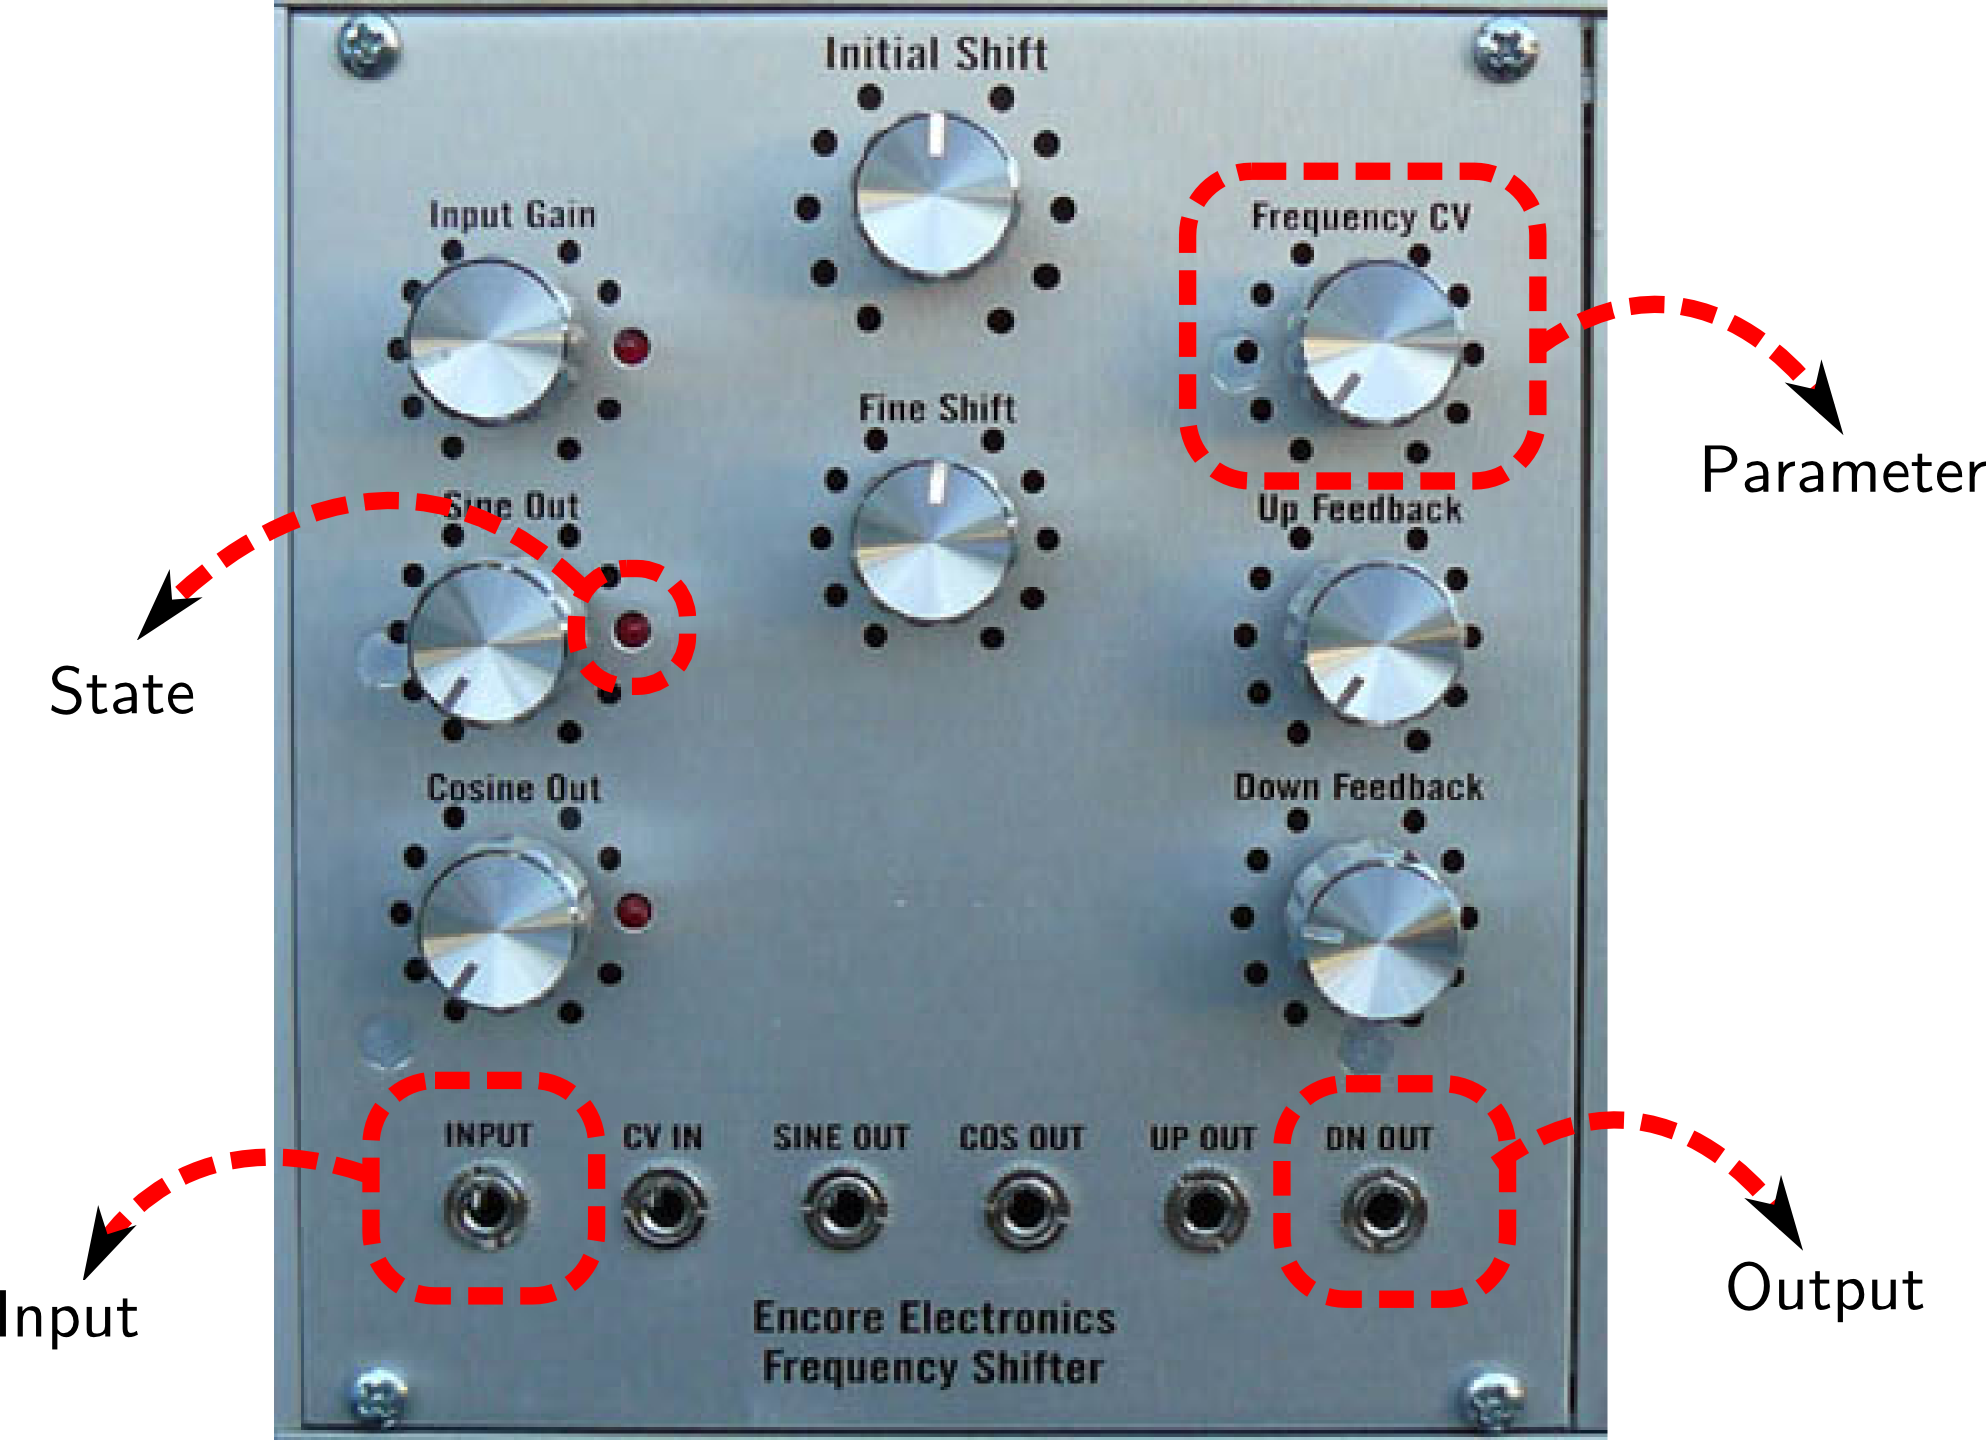
\includegraphics[width=.9\textwidth]{pic/hwmod.png}
  \caption{Components of a synthesis module illustrated in a standard
    \emph{frequency shifter}.}
  \label{fig:hwmod}
\end{figure}

A collection of modules and the connections among them is called a
\emph{patch}. In a hardware modular synthesiser, these are assembled
in special racks that have slots satisfying some standard to place the
modules in them --- for example, the module in the figure fits in
\emph{eurorack} slots. In many software synths, and specifically in
the one we are developing, patches can be arranged hierarchically. We
can visualise this as if we could put a whole rack into a black box
with holes to expose certain controls and ports to the outside, and
then place this box in a larger rack. This is very useful in a
software synthesiser; for example, one could build a complex patch out
of low-level processing primitives and expose a simplified
interface. Some software, like Reaktor, call these patches
\emph{instruments}. This arrangement can then be stored into a file
for later use. On the Internet one can find many collections of these
ready-to-use patches, and there are even commercial packages developed
by professional sound designers.

The \emph{conceptual class diagram} in figure \ref{fig:graphconcept}
summarises all this. Note that this is a conceptual class diagram, not
a design one, so there is not necessarily a direct match to the
classes in the actual code, not even terminologically.

\begin{figure}[h]
  \centering
  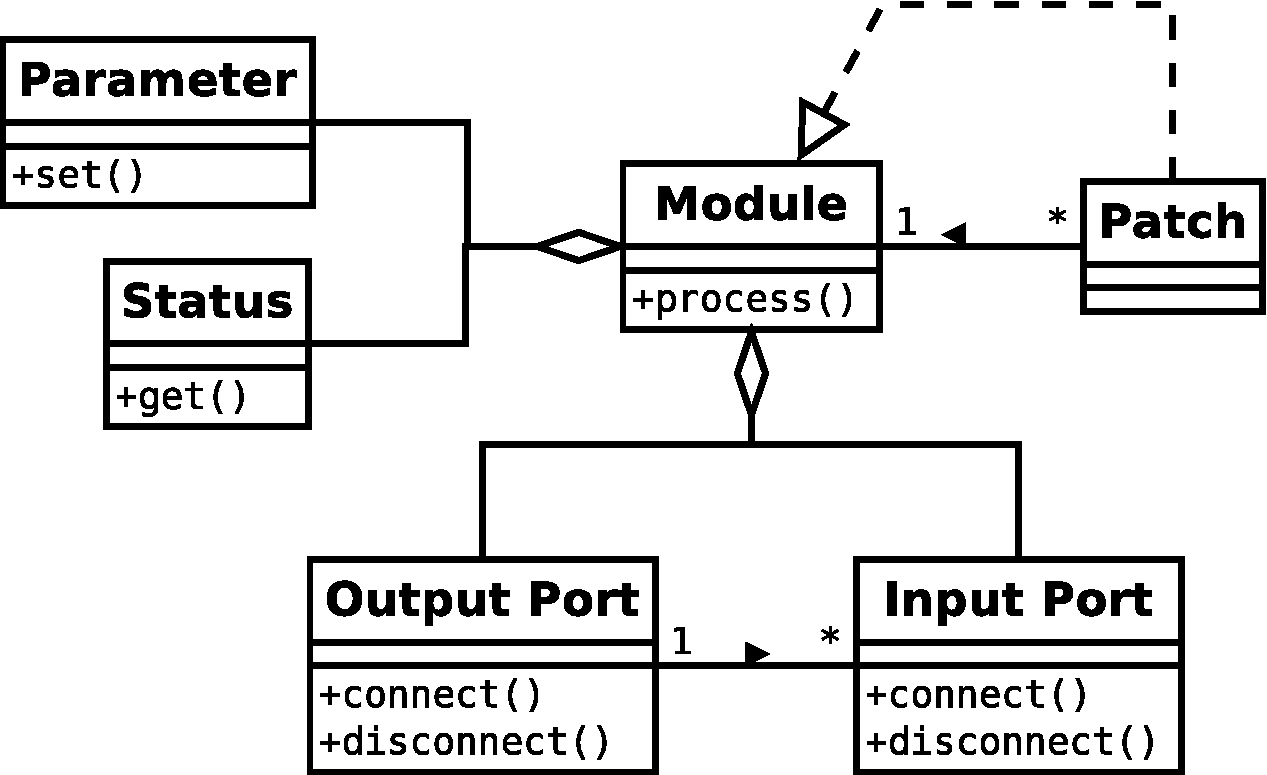
\includegraphics[width=.8\textwidth]{pic/graph-concept.pdf}
  \caption{Conceptual class diagram of the modular synthesis main
    entities.}
  \label{fig:graphconcept}
\end{figure}

\subsection{Software real time synthesis concerns}
\label{sec:rtsynth}

Our system generates the audio in real-time sending it directly to an
output device --- a sound-card. Even more, it is specially targeted at
live performances, so every operation should be designed such that it
does not disrupt the audio generation process and generates no kind of
noise. For example, in some software modular synths changing a
connection among ports triggers a recomputation of the dependencies
among modules to generate a compiled form of the patch for easier
execution; but that often that takes long enough to produce a small
buffer underrun --- i.e. an audible click --- as it might involve
doing non-linear computations or locking certain mutexes to
synchronise the state with the user thread. Actually, the port
reconnection issue requires special care, as we will discuss in
section \ref{sec:modports}. Because of \emph{dynamic-patching} we
should expect the topology of the synthesis graph to change a lot
during a live performance.

To better understand this problem we should understand how audio is
usually processed in real-time, thus feeding us with proper
terminology and knowledge to later tackle the issue. While this might
seem like a design issue to some, this is such a universal structure
that it shall be consider as a fixed constraint to be analysed than a
design decision itself.

Ideally, we would produce each sample one at a time and send it to the
output device. However, because we have to produce, at least, 44100
samples per second --- more in some professional applications ---
traversing all the synthesis system for every frame involves many
function calls, some of them even require dynamic dispatch in an
extensible system like ours, leading to a too low performance to
deliver the samples on time. For this reason, audio is processed
blocks of \emph{block size} samples in tight loops. This \emph{block
  size} might match the device's buffer size or it might be
smaller. Parameter and status values are updated only in between
blocks. Thus, we should try to keep the block size as low as possible
to avoid noticeable latency, and most professional audio software
allow changing this parameter to fit the machine processing power. A
sensible block size is 64 samples, like Pure Data's default. Using the
terminology in \cite{boulanger10audio}, we can distinguish between
\emph{audio rate} --- i.e. the frame rate as described in the previous
chapter --- and \emph{control rate}, which is the sampling frequency
of control signals --- i.e. the signals that produce only one sample
per processing block:

\begin{equation}
  control\_rate = \frac{audio\_rate}{block\_size}  
\end{equation}

Note that control signals are not restricted to what we labelled as
\emph{controls} in the previous sections. In fact, through a
\emph{port} may flow signals at audio rate if their signal type is
that of an audio buffer that holds a block of samples, or at control
rate if their signal type is that of a single sample, like a
\type{float} or \type{double}.

Interleaving the sound generation within the user-interface loop is
not plausible; thus the audio processing lives in its own thread/s. In
fact, as we saw in the last chapter, some audio output interfaces like
Jackd control the audio thread themselves invoking the processing
function through a callback. Our own device API wrapper that we
developed in the previous chapter promotes this kind of asynchronous
output and simulate it whenever the output system only provides a
blocking I/O interface. The inverse of the control rate, that we may
call the \emph{control period}, provides a very explicit deadline for
the block processing function. Missing the deadline might not kill
people, but it would produce an unpleasant clicking noise and thus we
have to do as much as possible to meet the deadline\footnote{In fact,
  in the middle of a live performance with a $10^5$ watts sound
  system, consequences might be more severe as it seems superficially
  :)}. Our system can be categorised as \emph{soft real-time}
\cite{tanenbaum07mos}. Apart from trying to get real-time priority in
the audio thread, we have to take special care when developing the
program, and this will deeply influence the design:

\begin{enumerate}

\item Avoid system calls in the audio thread. System calls produce a
  context switch and it can take quite long until the audio thread is
  preempted back; at least too much to meet the deadline. This is
  specially true for I/O system calls. In the previous chapter we
  already provided some devices to avoid this problem, like the
  caching file readers.

\item Avoid contending for a \emph{mutex} or some other kind of lock
  with the user thread. Without special support from the operating
  system --- like priority inheriting mutexes --- this can lead to
  priority inversion \cite{kim03basic}. Even in the later case, the
  context switch produced by the contention gives good chances to miss
  the deadline until the audio thread is preempted. The overhead of
  locking a mutex when there is no contention is negligible in most
  operating systems, and it definitely is in Linux which uses
  \emph{futexes} (Fast User-space Mutex) to implement them
  \cite{franke02futex}, so using a \emph{try-lock} operation is
  usually acceptable. The rule of thumb is to never wait on a mutex in
  the audio thread, and use lock-free data structures
  \cite{valois96lockfree} or do conditional locking instead.

\item Because the dead line depends directly on the block size $n$,
  algorithms running in the audio thread should be in $O(n)$. A special
  consequence of this restriction is that allocating memory in the
  heap, at least with the default allocator --- i.e. using \type{new}
  --- is forbidden. This is so because memory allocation algorithms
  are not proportional to the size of the requested block, but instead
  depend on non-deterministic properties like the pattern of memory
  usage and use complex search algorithms to find a fitting block of
  spare memory. This restriction implies that manipulating STL
  containers is forbidden too. For some special kinds of objects, like
  same-sized objects, a custom memory allocator can do the job
  \cite{alexandrescu01modern}. Sometimes, an intrusive data structure,
  like \emph{Boost.Intrusive} STL counterparts
  \footnote{\url{http://www.boost.org/doc/libs/release/doc/html/intrusive.html}}
  are enough to avoid the allocations. In other situations, we can
  release the job of allocating memory to the user thread, use custom
  data structures or any ad-hoc solution.
\end{enumerate}

\subsection{Anticipating future needs}

For the sake of proper workload balancing, several features that
deeply affect the structure of this layer are delayed for later
development iterations. However, to prevent rewriting the code at
those stages, we should anticipate what characteristics are
required from the basic constructs in order to later extend the system
with such features.

\subsubsection{Polyphony}

Polyphonic audio allows building chords and enrich the whole harmonic
depth of the music \cite{johnson02measured}. Polyphony is produced
when several notes are played at the same time; for example, by
pressing simultaneously several keys of a keyboard. Actually,
polyphony is also present without simultaneously pressing several
keys, as instruments usually have a significant \emph{decay time} ---
i.e. the time between the key release and the sound fully fades out
--- blending the sounds of successive key strokes.

Because in a modular synthesiser a generator is producing a single
tone at a time, it is not trivial to implement polyphony. In practice,
several copies of the processing graph are to be maintained, each one
is called a \emph{voice}. When a new note is to be played, the system
has to allocate a voice for it and trigger the processing; when it did
fully turn off the voice is released. Voice allocation is in many ways
similar to other allocation mechanisms, like page allocation in an
operating system, and different stragies have been proposed:
\emph{round-robin}, \emph{last-in-first-out}, \emph{priority based
  algorithms}, etc. The number of of voices is called the \emph{level
  of polyphony}, which is usually user-controllable but fixed during a
performance parameter of the system. In practice, modern computers
allow levels of polyphony high enough (from 16 to 128) such that the
sophistication of the allocation mechanism is not relevant for the
overall qualitative experience of the overall sound produced by the
synthesiser. Also, in a modular software synthesis engine, a whole
network needn't be polyphonic. For example, some dynamic range
compression or reverb filters are usually applied to the final mixed
sound of all voices, yielding better performance but also a richer
sound.

It is not worth to concentrate on the actual management of the
different voices and the triggering mechanisms until sequencing and or
MIDI support is developed in later stages. However, there are some
questions that we do have to address now:
\begin{itemize}
\item We have to split the responsibilities of the different classes
properly predicting which classes will need to be extended, preferably
via inheritance, to provide the polyphony support.

\item We have to define, at least partially, an interface that
  polyphony enabled DSP nodes will have to implement.
\end{itemize}

\subsubsection{Plug-in system}

At a later stage, we plan to implement a plug-in system as defined by
requirements \ref{req:iter3-begin} to \ref{req:iter3-end}. These
plug-ins shall be in several formats, like LV2, LADSPA, or our own
defined interface. We should take this in several ways:
\begin{enumerate}
\item For consistency, the interface that we will define in this
  chapter shall be the same that our own plug-ins will implement
  later. The only significant difference should be the linking method
  of the code and the registration mechanism.

\item Object construction, even for statically linked DSP modules,
  should be done in an indirect way, via object \emph{factories}
  \cite{gamma95design}. Thanks to this, the system can later be
  transparently extended by modifying the factory object to delegate
  the construction of specially-identified objects --- objects
  identified by a resource URI \cite{mealling02rfc3305} --- to a plug-in
  loader.

\item Parameters, states, inputs and outputs of an object should
  accessed via dynamic means of introspection. In practise, they
  should be identified by strings ands modules should provide some way
  of iterating through them. Ideally, there should be some hooks to
  provide some meta-data that can be useful for an automatic user
  interface builder; for example, a parameter's range, whether it is
  naturally linear or logarithmic, etc.
\end{enumerate}

\section{Design}

\subsection{Overview}

Figure \ref{fig:graphoverview} shows an overview of the most important
classes in this layer from the musical point of view. Most of the code
implementing these classes lives in the \type{psynth::graph}
namespace, representing the fact that this layer implements the notion
of sound processing described a graph on interconnected processing
modules. The \type{node} class is the base class of all kinds of
vertexes in this graph. Therefore, \emph{node} is a synonym for what
we called \emph{module} or \emph{DSP node} in the analysis section;
i.e. it is the basic unit that processes some input signals producing
new output values. In the rest of this chapter, unless otherwise
stated in its close context, we will use the term node with this
meaning.\footnote{Indeed, we prefer this term as the name
  \emph{module} has a different specific meaning in the code, similar
  to that of \emph{translation unit}, as we describe in the
  ``Programmer guide'' addendum.}

\begin{figure}[h]
  \centering
  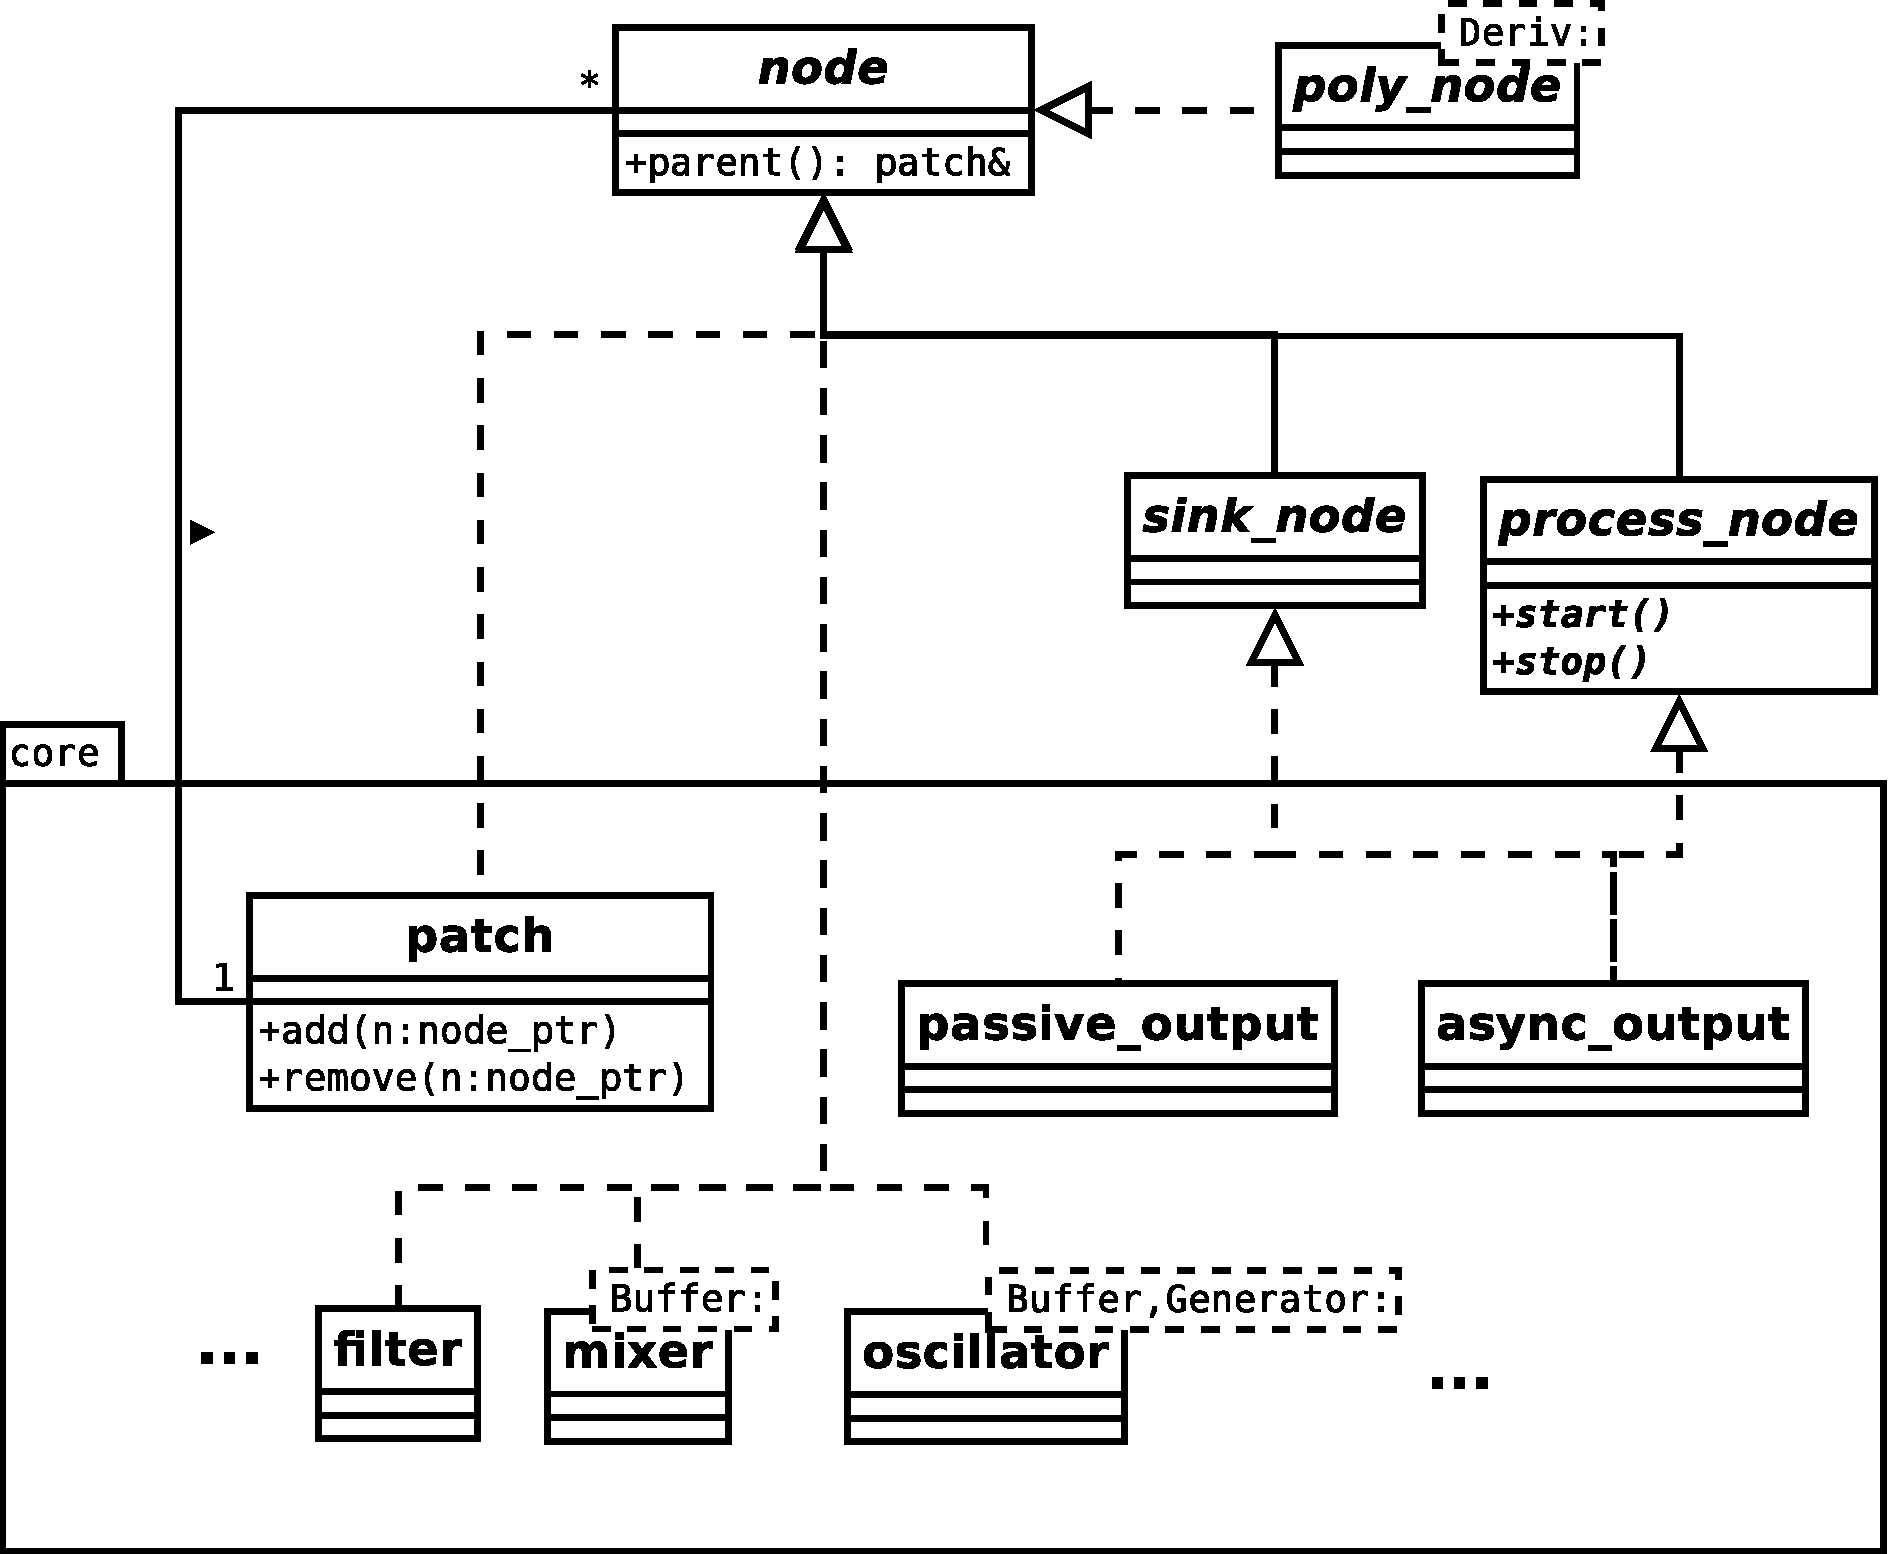
\includegraphics[width=\textwidth]{pic/graph-node.pdf}
  \caption{Overview of the graph layer}
  \label{fig:graphoverview}
\end{figure}

The \type{psynth::graph::core} namespace contains the \emph{concrete}
nodes that are implemented in our library. All these shall be
registered in the object factory that we will describe in section
\ref{sec:graphfactory} and most of the code should not instantiate
these modules directly. This introduces the notion of \emph{core
  node}, i.e. a node that is built-in --- statically linked --- inside
the library, thus is not a plug-in. Other sorts of abstract nodes that
are there only to offer certain functionality should live directly in
the \type{psynth::graph} namespace as they are considered basic
infrastructure and may be useful in the implementation of plug-ins.

We will explain other parts of this diagram later. What should be
clear now is the relationship between a \type{node} and a
\type{patch}. This is an instance of the \emph{composite} design
pattern \cite{gamma95design, vlissides98pattern}. A \emph{patch} is a
collection of nodes but it is a node by itself, building tree-like
structures that most of the time have non-patch nodes as leafs, and a
patch on its root. To ease memory management, \type{node\_ptr} is an
alias for \type{std::shared\_ptr<node>}\footnote{This is a recurring
  pattern, also explained in the ``Programmer guide''}. A node keeps a
weak reference to its parent easing traversal and some special
operations, accessible via the \type{parent ()} method.

We will next explain the execution model of the synthesis network
defined by these classes, but first, lets make a parenthesis to
explain a novel data-structure that is deep in its core.

\subsection{Heterogeneous deques --- bridging polymorphism and
  real-time processing}

As we explained in the analysis section, avoiding heap allocation is
crucial in real-time processes. Proper runtime polymorphism is said to
require heap allocation because the code paths in charge of managing
the lifetime of some object do not know its full type --- specially
the actual object size --- and thus the object can not be allocated in
the stack. While true in general, we can constrain the problem in
several ways to obtain $O (1)$ allocations if the programming language
provides enough low level constructs to implement these solutions.

A possible solution is to override the operator \type{new} for certain
types to provide constant-time allocation. Alexandrescu provides a
clever way of doing this here \cite{alexandrescu01modern}. This,
however, have several problems:

\begin{enumerate}
\item \emph{Concurrency}. We have, in general, several threads
  creating objects of these kinds. Alexandrescu solves the problem by
  using mutexes. This is forbidden in our real-time thread; which is
  just what we are trying to avoid. Maybe a lock-free data-structure
  could be used to allocate this memory, solving the issue, but we do
  not know about it.

\item \emph{Explicitness}. We would like to easily know what
  operations are safe to be performed in the real-time thread. Any
  programmer should get worried when he reads something like this in a
  real-time code path:
  \begin{lstlisting}
    some_type* x = new some_concrete_type (...)
  \end{lstlisting}
  To regain confidence about the correctness
  of that code, he should go and read the implementation of
  \type{some\_\-concrete\_\-type} and discover that it has an
  overloaded operator \type{new}.
\end{enumerate}

Another plausible solution is to constrain the set of types acceptable
in some variable. By doing so we are, in fact, changing the open world
assumption of universal polymorphism by the closed-world assumption of
ad-hoc polymorphism. Thanks to this constrain, we can, via template
metaprogramming or the new C++11 \texttt{constexpr} facility, compute
at compile time the maximum storage needed to hold values of any of
those types and allocate it in the stack; then construct the objects
in this space with \emph{placement new}. This is actually how
\emph{Boost.Variant}\footnote{\url{www.boost.org/doc/html/variant.html}}
is implemented \cite{alexandrescu01unions}, and as we are depending on
Boost already, using it is quite safe in real-time code and can be a
solution when ad-hoc polymorphism is enough.

In some other cases ad-hoc polymorphism is not enough, but the pattern
of object construction and destruction can be constrained instead. We
can think of \emph{the heap} as a global data-structure --- a
data-structure that is so useful that its insertion and deletion
operations are keywords of the language itself, let them be the
operators \type{new} and \type{delete}. In fact, its interface is very
similar to that of a multi-set, but without iteration and with the
ability to hold elements of varying size. If we restrict its interface
such that elements can only be allocated and released in FIFO or
LIFO order, we get a \emph{deque}. 

\begin{lstlisting}[float=h!,caption=Example of usage of heterogeneous deques,label=lst:heteroexample]
  struct base {
      virtual void method () { std::cout << "b"; };
  };
  struct deriv : base { 
      deriv (int x = 0)      {} 
      virtual void method () { std::cout << "d"; };
  };

  hetero_deque<base> q;
  base b;
  deriv d;

  // 1. Copying
  q.push_back (b); q.push_front (d);

  // 2. Moving
  q.push_back (deriv ()); q.push_front (std::move (b))

  // 3. Constructing, even with params!
  q.push_back<base> (); q.push_front<deriv> (1);

  // Error checking
  // static_assert error: 'int' is not a subtype of 'base'
  q.push_back (1); 

  // Access is polymorphic!
  // Output: bddbbd
  for (Base& x : q)
    q.method ();
\end{lstlisting}

The class \type{psynth::\-ba\-se::\-he\-te\-ro\_de\-que<Base>} is a
cons\-tant-size deque that can hold elements of any subclass of its type
parameter \type{Base}. The concrete type of the object must be known
at insertion time for the deque to be able to allocate space for it in
its internal buffer. Actually, the data structure API offers three
ways of inserting an concrete derivate of \type{Base} into it, (1)
copying it, (2) moving it using R-value references or (3) directly
constructing it into the data-structure, using perfect forwarding to
pass the parameters. It is statically checked that the inserted
element is a subtype of \type{Base}. All this is illustrated by the
example in listing \ref{lst:heteroexample}.

The data-structure interface is similar to that of an STL deque, with
some differences. Because access is done polymorphically via a
reference of type \type{Base\&}, \type{value\_type} semantics, which
maps to \type{Base}, are slightly different than in most containers
because the actual elements are of different heterogeneous concrete
types. Also, because objects can be directly constructed inside the
data structure with arbitrary parameters, they needn't be regular in
any sense, this is, they don't have to be copy-constructible,
move-constructible, default-constructible, copyable or moveable. This
is quite convenient because classes that are designed to be used
polymorphically more often than not do not satisfy many of these
properties. The only restriction is that \type{base} should have a
virtual destructor if any of its derivates has a non-trivial
destructor.

Note that the data structure itself is not copyable, nor moveable, nor
resizeable. While this is feasible it has a slight memory overhead
and, as our current use-cases do not need it, we decided to stick to
the current simpler implementation. This is so because to be standard
compliant, an object identity --- i.e. the memory address where it
lives --- must remain constant during its livetime; in order to copy
or move it, we need to call the proper copy or move constructor, and
in the later case call the destructor of the moved object if it is to
be released \cite{cppstd}. Calling the proper copy or move operation
requires, at least, one function pointer --- or a \emph{vtable}
pointer for a box type. We already have a plan to implement this
feature using policy-based design \cite{alexandrescu01modern} such
that it does not cause an overhead to those who do not need it.

\begin{lstlisting}[float=h!,caption=Header of heterogeneous deque elements,label=lst:heteroheader]
  template <class Base>
  struct header {
      header* prev;
      header* next;
      Base* access;
  };
\end{lstlisting}

The data structure is implemented by storing the objects in a constant
sized memory block organised in a circular buffer fashion.  We append
a header like the one in listing \ref{lst:heteroheader} at the
beginning of each a object. An empty header at the end of the list
allows to keep track of the beginning of the free space. The
\type{prev} and \type{next} pointers organise the data in the deque in
a doubly-linked list fashion. Even though the storage is continuous,
this is needed because the size of the objects is variable and only
known at object insertion time. The \type{access} pointer keeps a
reference to the object itself casted to \type{Base*}. This is
required because, in the presence of multiple-inheritance, the
\type{Base} part of the object might not be aligned at the beginning
of the object's layout. If we think about it, the \type{next} and
\emph{access} pointers are just a way of keeping track of the
static information that is lost in the \emph{type erasure}
that happens when adding a new element to the data structure: its
\emph{size} and the \emph{offset} to its still known attributes and
\emph{vtable}; the \type{prev} pointer just aids reverse traversal and
addition at the front.

Figure \ref{fig:heterostructure} represents an instance of the data
structure containing two objects. The \type{front} and \type{back}
pointers keep track of the first and last valid element in the
container. We can see how adding a new element that does not fit at
the end of the memory space, causes that space to be wasted ---marked
as \emph{offset} in the figure---  and the object is instead added at
the beginning of the memory block, where there is enough free space
available in this case, in a circular buffer fashion.

\begin{figure}[h!]
  \centering
  \subfloat[]{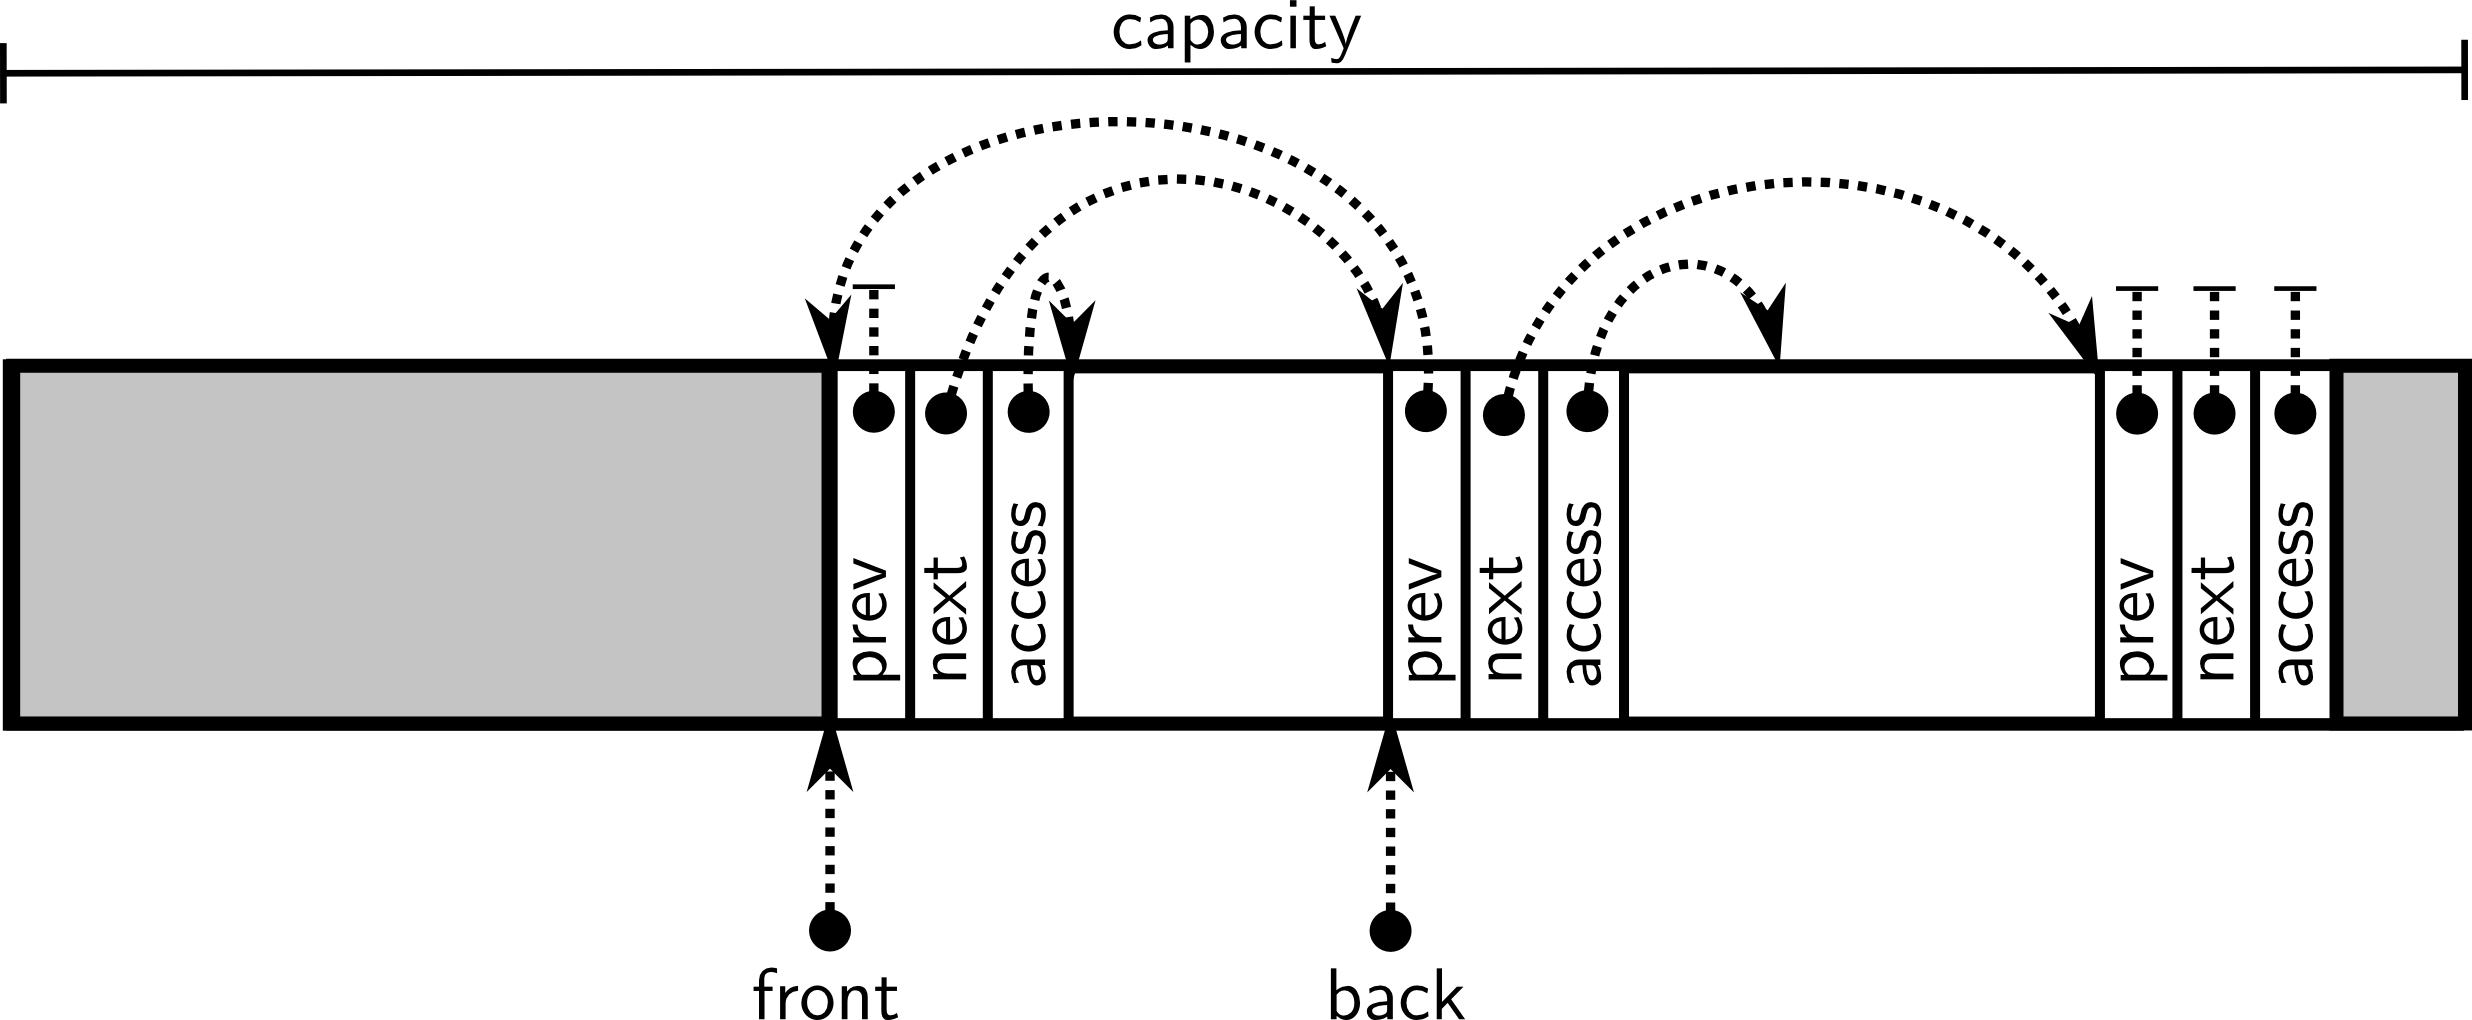
\includegraphics[width=.95\textwidth]{pic/hetero1.png}}

  \subfloat[]{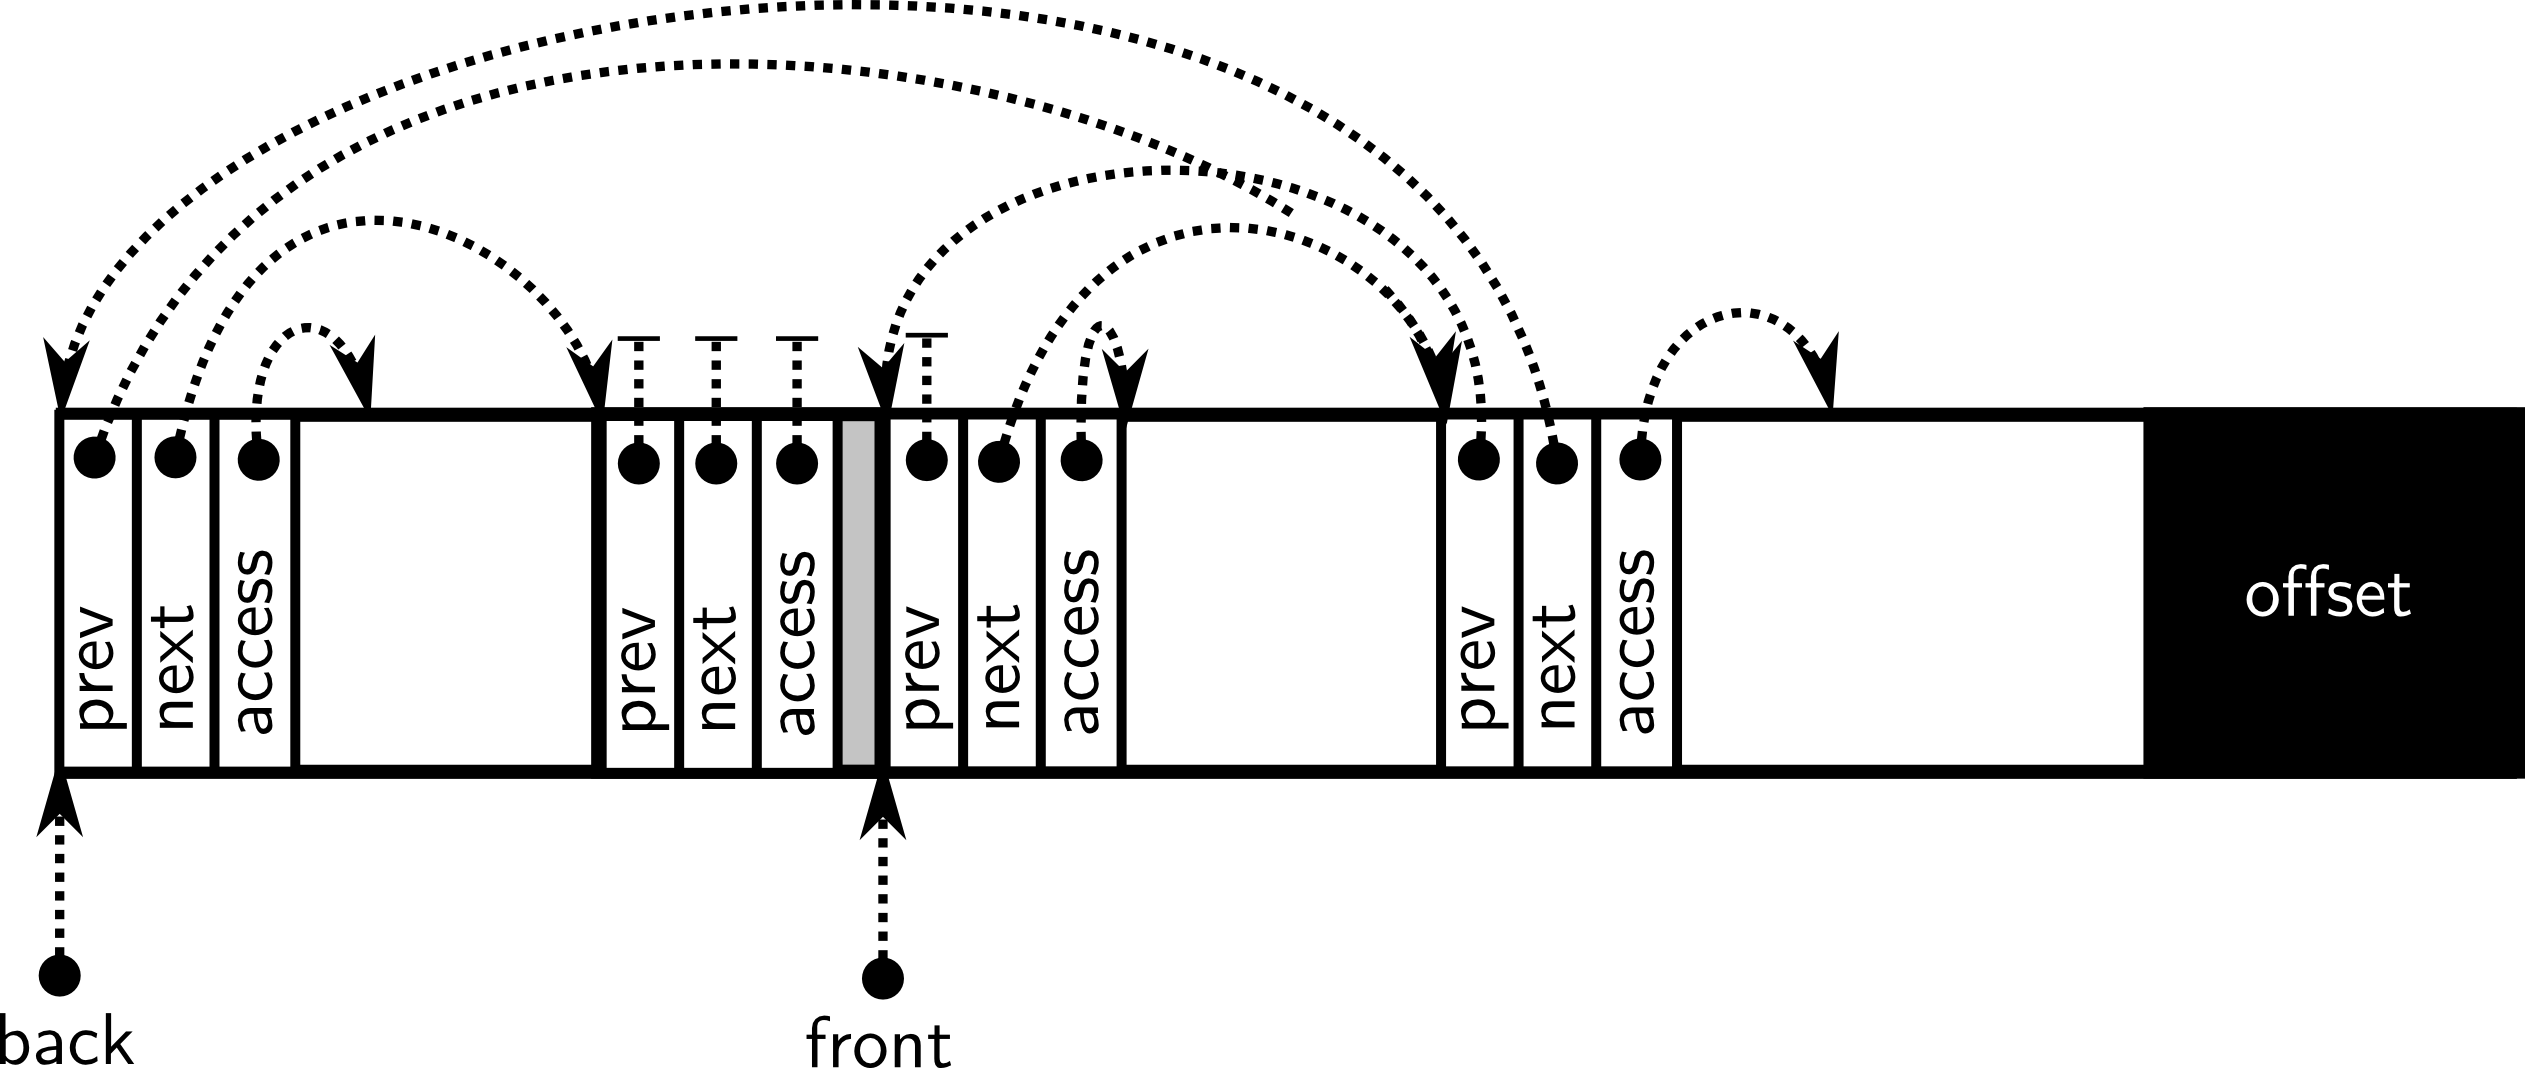
\includegraphics[width=\textwidth]{pic/hetero2.png}}

  \caption{An heterogeneous deque with two elements (a), and after
    adding a third element (b).}
  \label{fig:heterostructure}
\end{figure}

So, thanks to low level facilities provide by C++, we are able to use
different techniques to get the benefit in expressiveness and
maintainability of polymorphism in a real-time constrained
environment. Our most prominent use-case, passing active events among
different threads, gets very benefited from our last approach, as we
shall see in the rest of this section. In other parts of the system,
disjoint unions as implemented by \emph{Boost.Variant} are enough, and
we actually do use them to treat a closed family of oscillator objects
polymorphically in our oscillator node implementation. A custom object
allocator is a valid solution in some other situations, but as we have
already analysed, it is mostly unsuitable for our quite specific
needs.

\subsection{Execution model}

\begin{figure}[h]
  \centering
  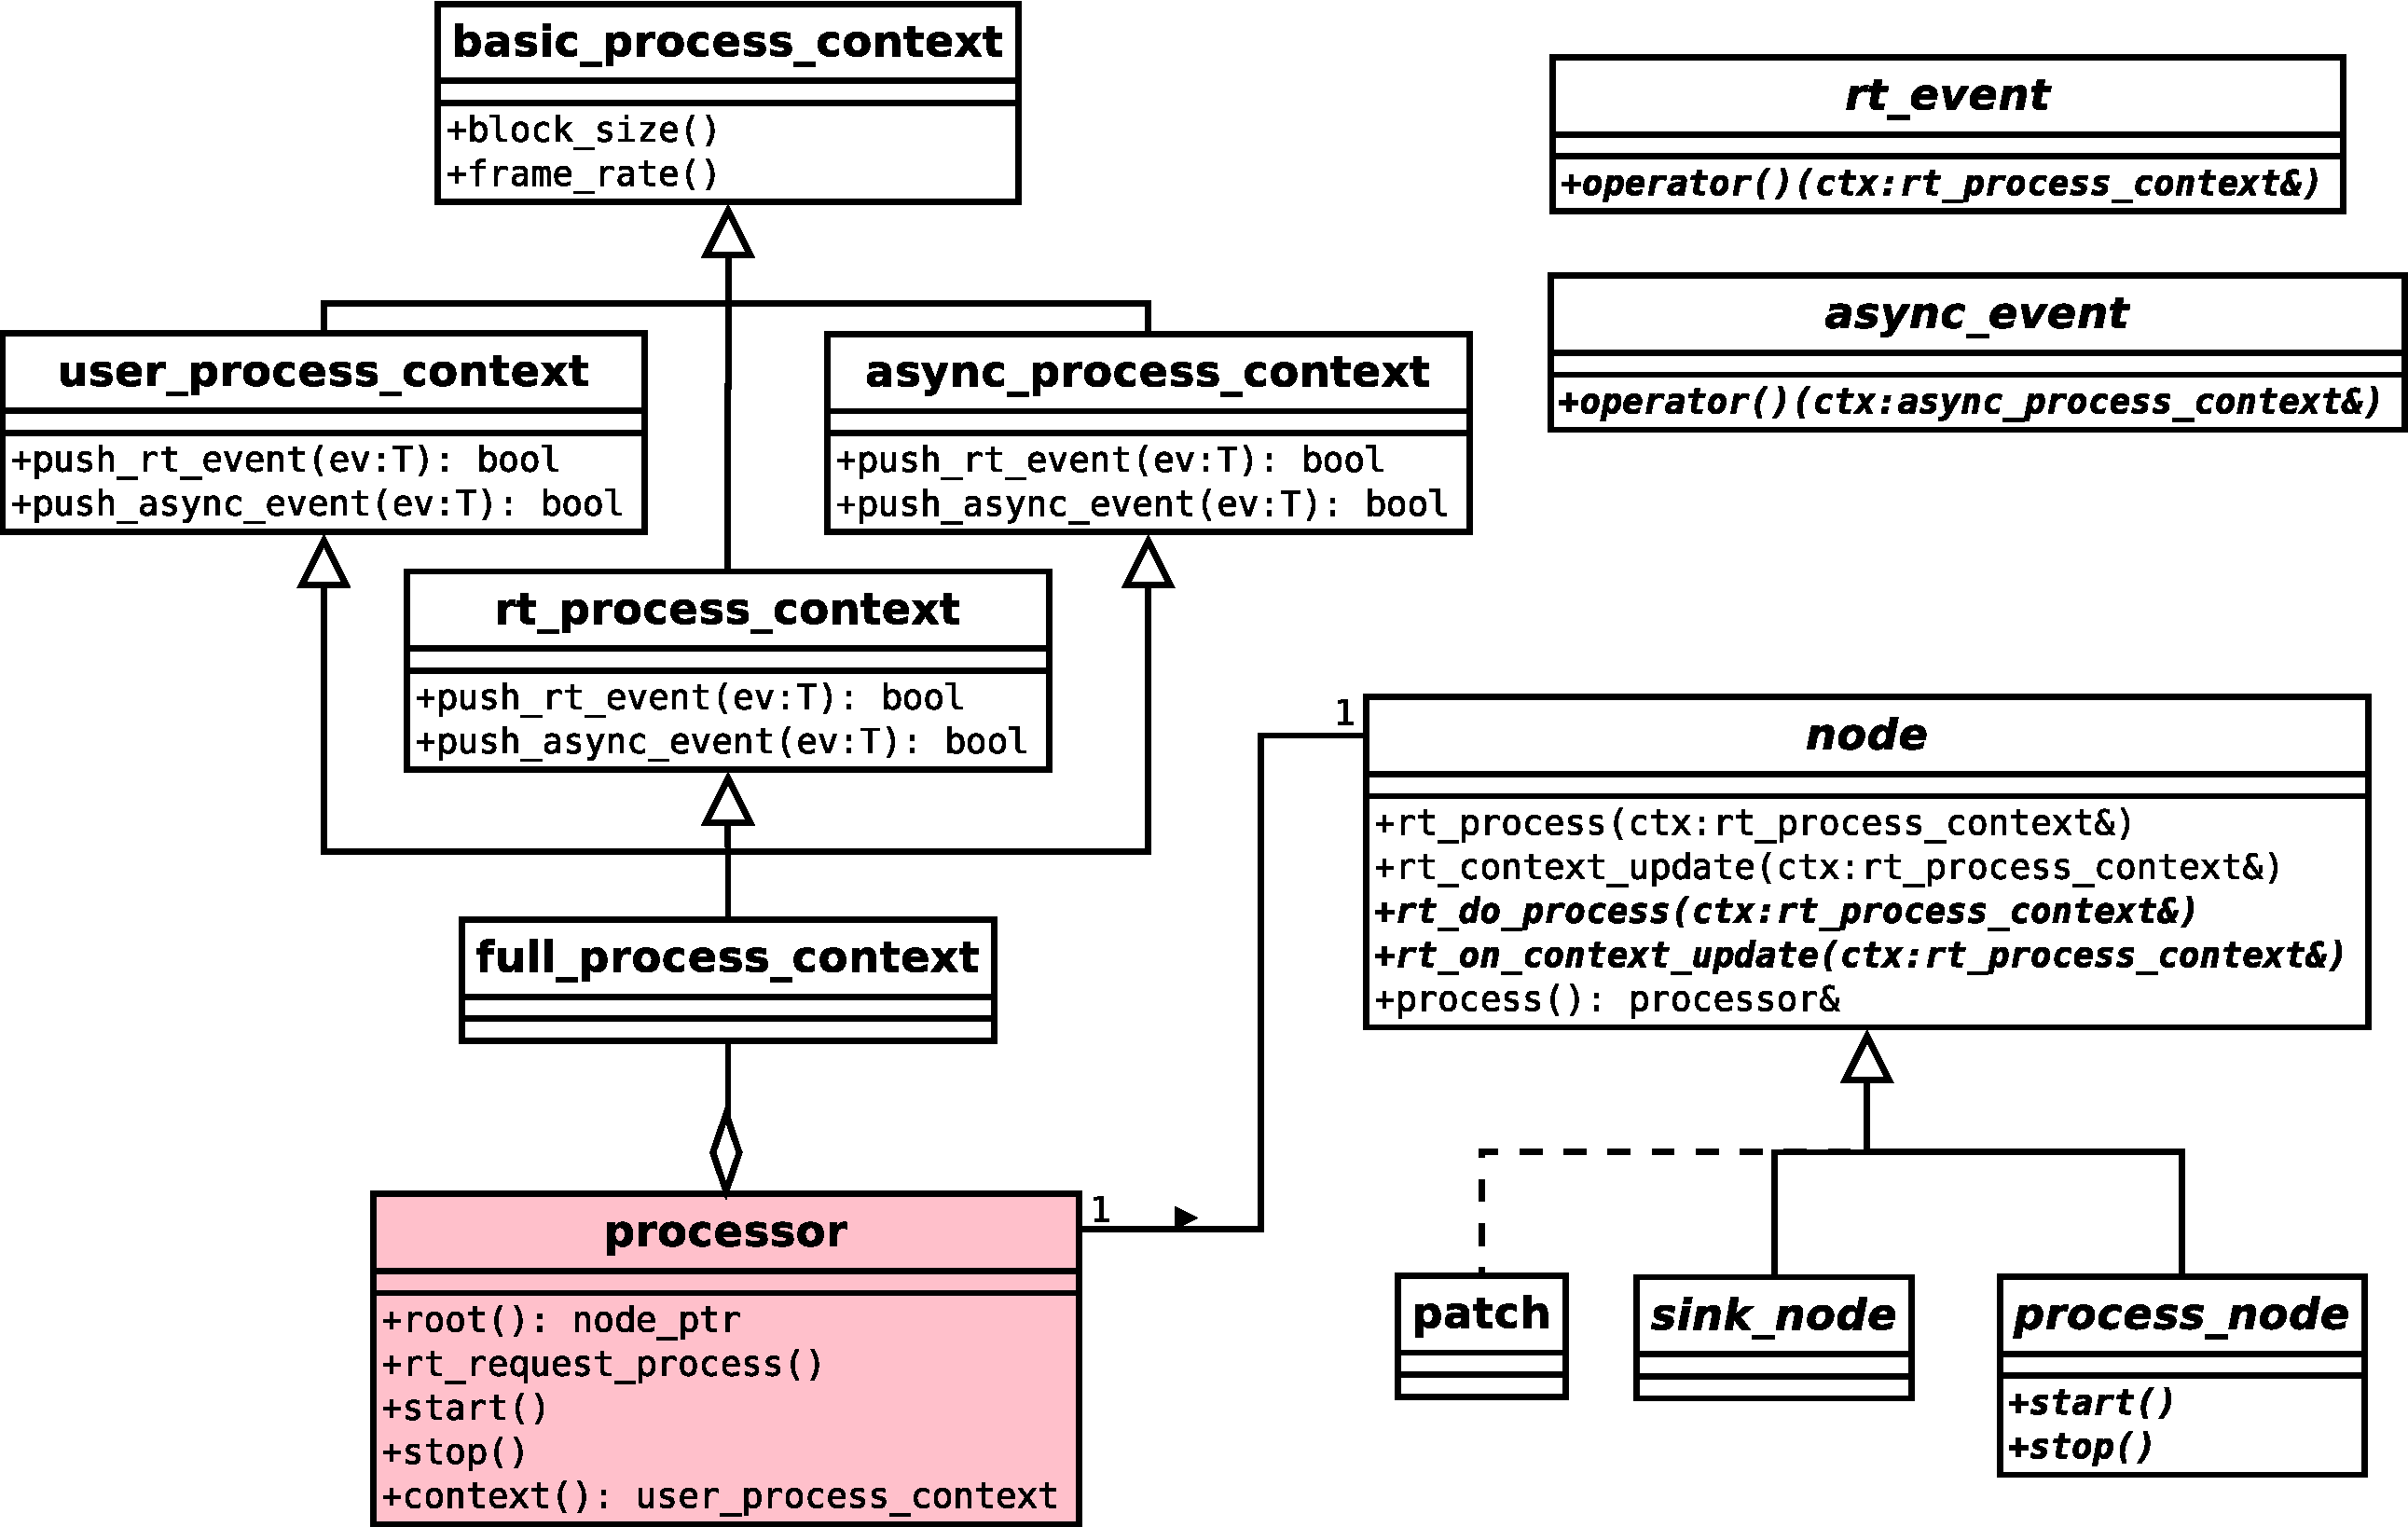
\includegraphics[width=\textwidth]{pic/graph-processor.pdf}
  \caption{The graph processor, its context and the processing methods
    of nodes. }
  \label{fig:graphprocess}
\end{figure}

Figure \ref{fig:graphprocess} introduces some new classes that are the
coordinate the execution of the synthesis graph. Because there are
several concurrent ---and potentially parallel--- threads of
execution, writing code without race conditions and other
synchronisation problems can get quite hard if we do not establish
some conventions. Unless otherwise specified in its documentation, a
method is expected to be executed in only one \emph{kind} of thread,
sometimes even in just only one specific thread. There are three kinds
of threads and some naming conventions allow us to determine in which
thread some method is expected to be used:

\begin{description}
\item[User thread] The user thread is the one where most objects are
  created and where usually the user interface lives. In some way,
  this can be considered the \emph{normal thread}, and it is the root
  of the thread tree --- i.e. the one that creates the other threads.

  If a method does not have any special prefix nor belongs to a class
  named with a special prefix, we shall assume, unless otherwise
  specified in its documentation, that it is safe to execute it only
  in the user thread. In the current implementation, these methods,
  while reentrant, they are not fully thread-safe. This means that
  most non-const methods of an object and related objects
  ---i.e. objects that keep references among themselves--- shall be
  executed in the same thread, but it is safe to operate with
  unrelated objects in different user threads.

\item[Real-Time (RT) threads] These are the threads where the actual
  work of processing the synthesis graph is done. As we shall see
  later, these threads are controlled by the \type{process\_node}
  derivates, but that is not relevant now. Methods beginning by the
  \type{rt\_} prefix, and all methods of classes named with that
  prefix, are expected to be executed in this thread. While it can be
  normal for several RT threads to coexist, implementers of RT-methods
  and objects should not worry about this, because, unless they are
  actually implementing a \type{process\_node}, the system itself
  serialises calls to dependent methods --- in the current
  implementation, it just serialises calls to
  \type{rt\_request\_process}, we will discuss this soon.

\item[Asynchronous operation threads] These threads, that we
  may call just \emph{async threads}, ease the execution of operations
  that are forbidden in the RT thread. The \type{processor} controls
  the execution of these threads. Methods and classes prefixed with
  \type{async\_} are expected to be executed in these thread.
\end{description}

\subsubsection{Processing the graph}

The \type{processor} class is a \emph{fecade} that manages the
execution of the synthesis graph described by a given root node. Of
course, a whole graph can be attached to one and only processor and an
exception would be thrown if we try to attach it to several.

\begin{algorithm}
  \caption{Process a control iteration of the graph, $rt\_process (n,
    ctx)$}
\label{alg:processgraph}
\begin{algorithmic}
  \REQUIRE $\;$\\
  $n \in \mbox{\type{node}}$ \\
  $ctx \in \mbox{\type{rt\_process\_context}}$
  \ENSURE $\;$\\Every node in the graph is processed and its results ready in their
  outputs, if any, in the right order.
  \medskip
  \IF{$\lnot visited (n)$}
  \FORALL{$i \in inputs (n)$}
  \IF{$connected (i)$}
  \STATE $n_i \gets source (i)$
  \STATE $rt\_process (n_i, ctx)$
  \ENDIF
  \ENDFOR
  \STATE $rt\_do\_process (n, ctx)$
  \STATE $visited (n) \gets \top$
  \ENDIF
\end{algorithmic}
\end{algorithm}

The \type{rt\_request\_process} method triggers the execution of one
iteration of the graph, this is, it processes one block of audio rate
samples or one control sample. The processing algorithm is as
follows. The processor keeps a list the nodes that have side-effects
outside the graph itself, for example, an node for outputting to a
device. These are the nodes that inherit from \type{sink\_node}, and
we can refer to them as just \emph{sinks}. For every sink, the
processor invokes the recursive algorithm \ref{alg:processgraph}
implemented by \type{rt\_process} in the \type{node} class. This
recursively calls the process method of the nodes connected to one's
input. Because the synthesis graph may have loops and input ports may
be connected to several outputs, it marks every node it visits. In
this way, every node is processed only once and nodes that may have no
side effects are discarded --- because they do not interact wit the
``real world'' nor any node that does depends on it. When a node is
being visited, the pure virtual \type{rt\_do\_process} methods is
invoked. That is the most important method that implementers of
their DSP modules have to take care of; in it they should fetch the
input data, if any, process it, and write some output, if any. We
often just call this the \emph{worker method} of a node.

\subsubsection{Proactive nodes}

\type{rt\_do\_process} is usually executed by implicitly triggered by
\emph{process\_nodes}. These nodes represent devices that may require
processing from the graph have and extra \type{start ()} and
\type{stop ()} method. They are in charge of managing their own thread
where they request processing whenever they need frames.

A canonical concrete \emph{process\_node} is
\emph{core::async\_output}, which, when associated to an asynchronous
output device (see section \ref{sec:asyncio}), requests processing in
the output callback and passes what it gets from its single input port
to the device. In order to allow several asynchronous output devices,
calls to \type{rt\_request\_process} are serialised. Then, in their
worker method they just accumulate their input in an internal ring
buffer, but not directly output to the device, because that operation
may block and delay other devices that are waiting on this request. In
their own device callback, when there is enough information in their
internal ring buffer, this is sent to the device.

Calls to \type{rt\_request\_process} are serialised using a mutex in a
special way. When we try to get the lock and is owned already, we do
wait for the ongoing request to finish, but we do not perform a new
request, because the one that was already on the way might have been
enough for the device to get sufficient information. This use of locks
does not violate the RT rules, because all threads that are expected
to contend for it are real-time so no priority inversion can occur. It
may introduce some context switches, but that is unavoidable, and in
practise they do not add much overhead, and in modern processor the
gained parallelism compensates. While we are doing the output
operation on the device, another process node might have triggered
another request, preparing our next bunch of frames already. When we
are locked on the mutex, another RT thread is already doing what we
wanted to do, and if the OS scheduler is not dumb, it should preempt
our RT thread soon at it will happily find that its request have been
processed already. Thanks to this mechanism we can output to several
devices at the same time, even if they are in different sound
cards. What is output to each one depends on how the graph is
interconnected, and it might even be different. This is a common
usecase, for example, DJ's peek at how it the next track mix's in
while they adjust its tempo on their headphones without altering what
is still being played on the loudspeakers. Figure \ref{fig:djscheme}
shows how a typical DJ setup could be built with Pyschosynth's engine
and illustrates the most important aspects of the algorithm that we
just described.

\begin{figure}[h!]
  \centering
  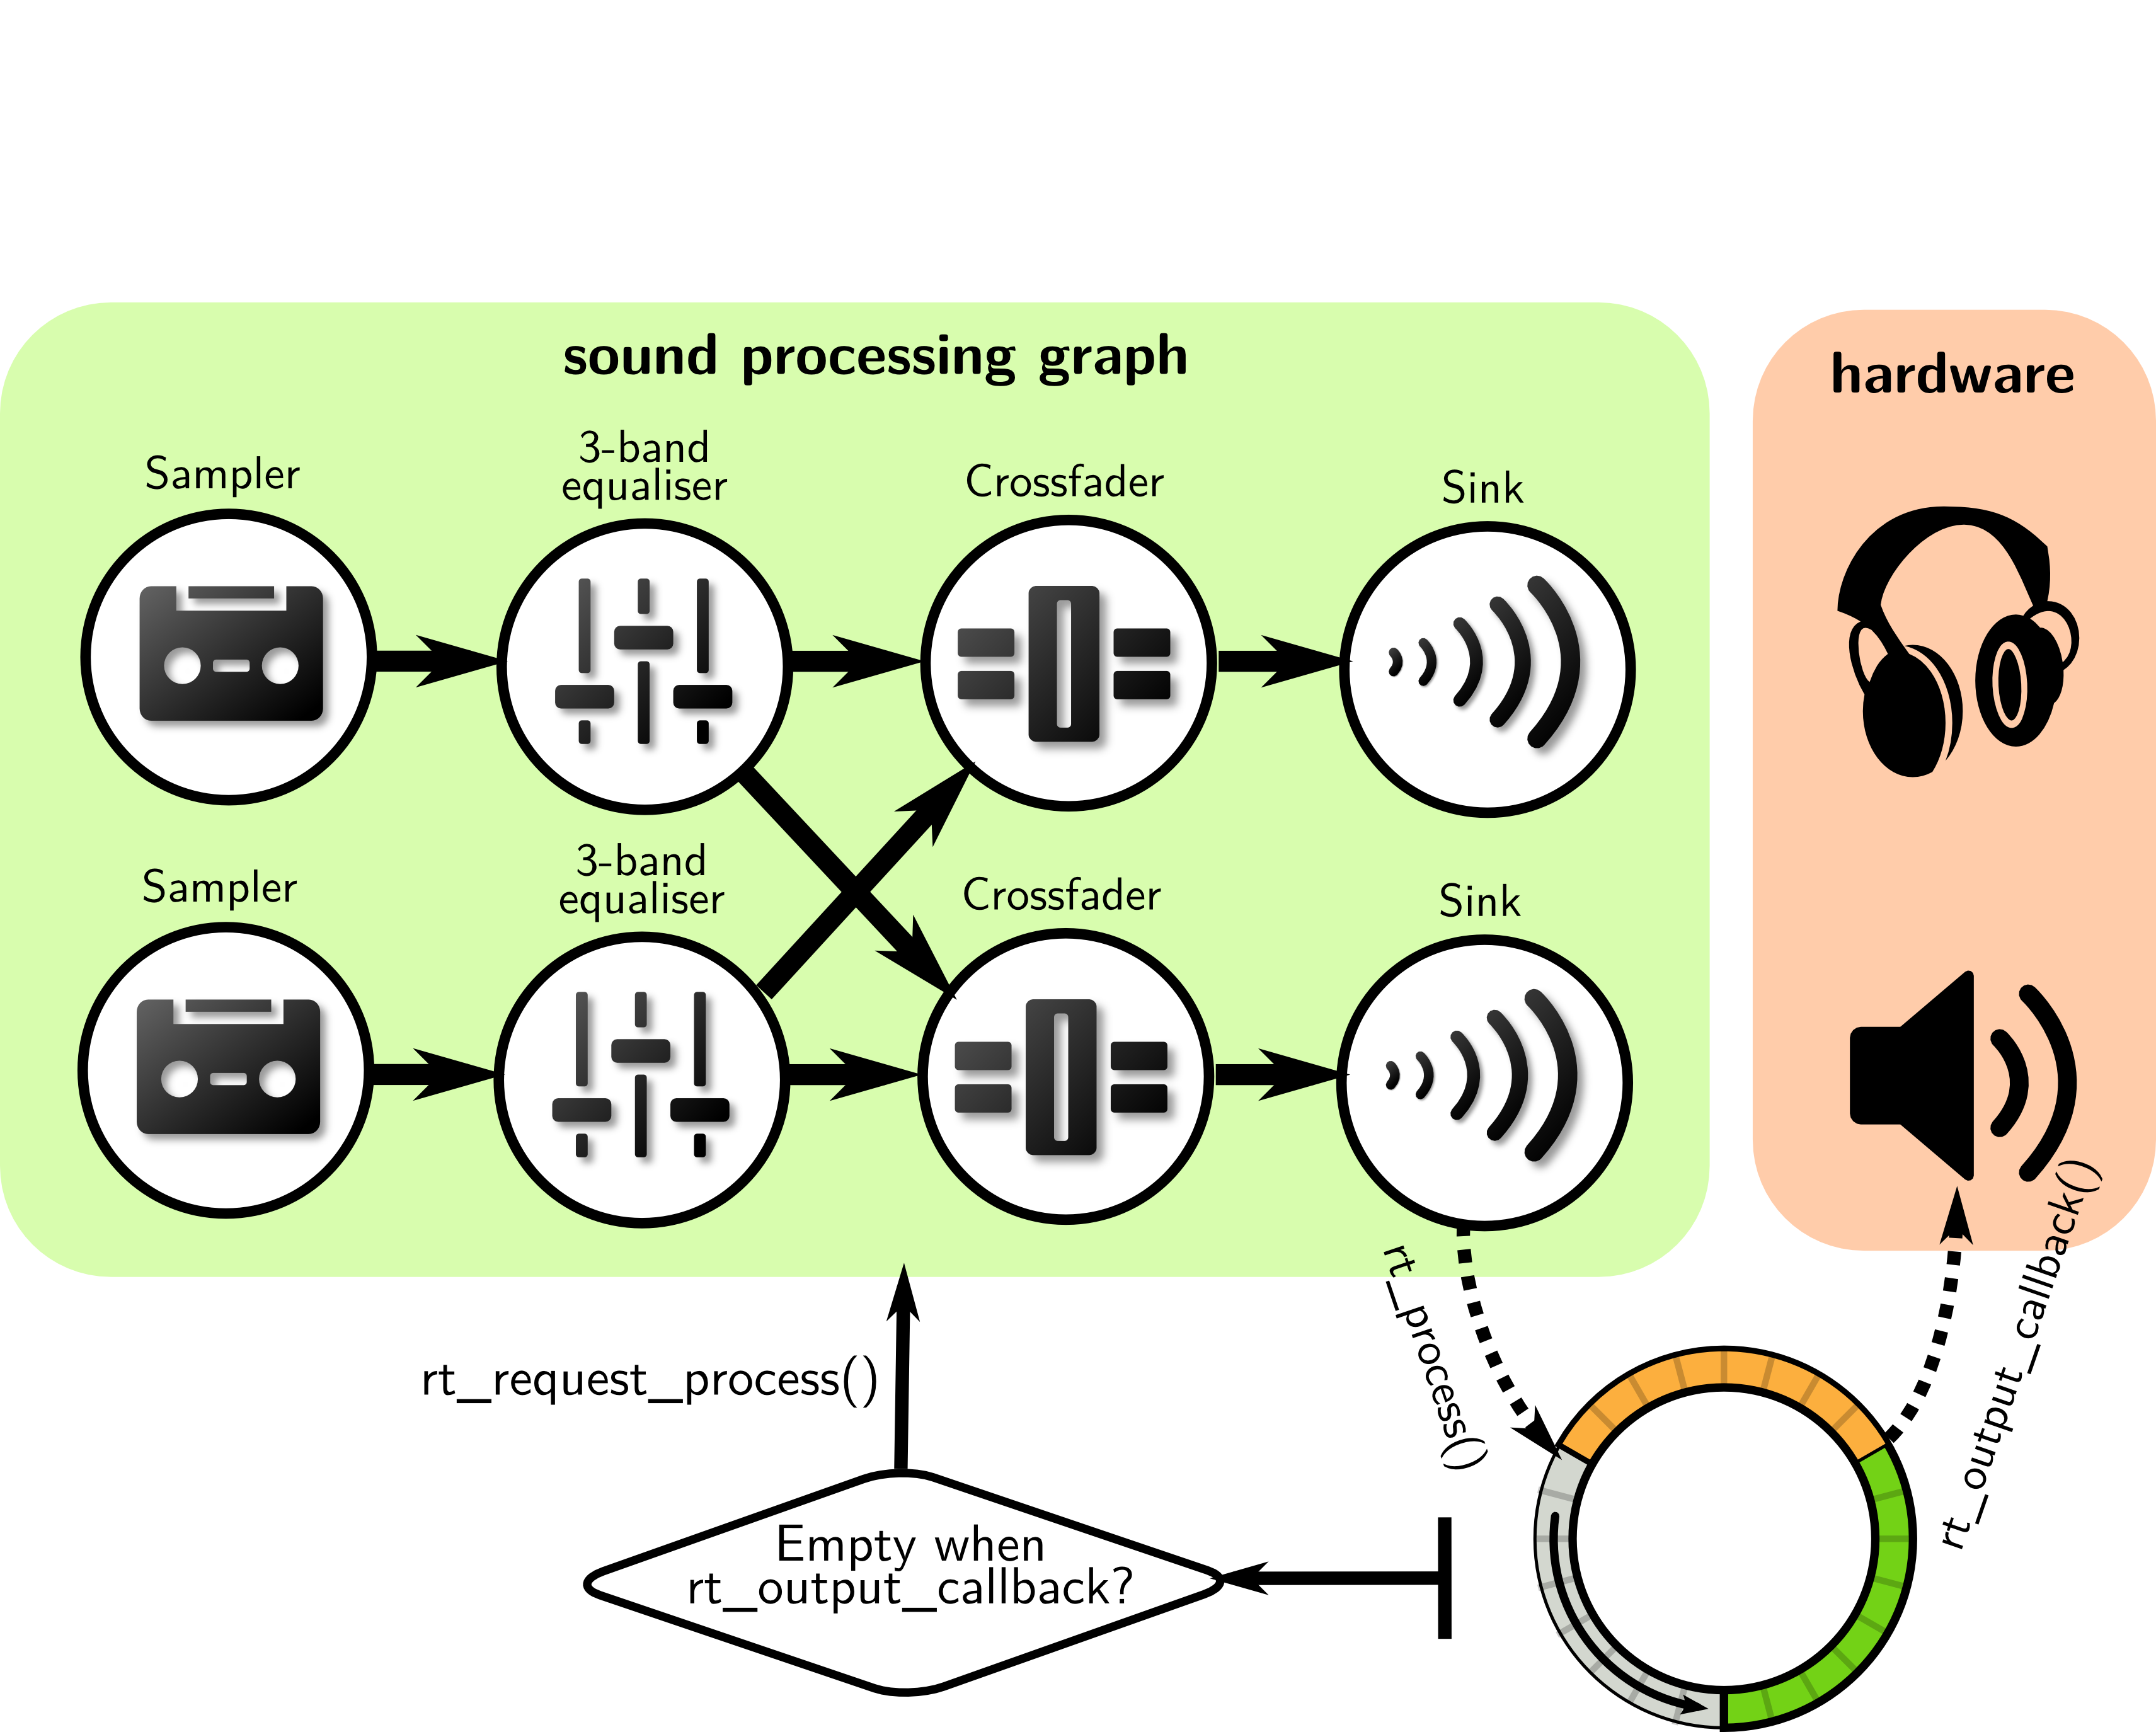
\includegraphics[width=\textwidth]{pic/djscheme.png}
  \caption{A DJ setup built with Psychosynht's engine to illustrate the multiple device output system.}
  \label{fig:djscheme}
\end{figure}

The \type{start ()} and \type{stop ()} methods in the \type{processor}
class is in charge of starting and stopping all the process nodes in
its associated graph. It also starts nodes that are added after the
processor have already been started and stops them when
removed. Usually, we can just start the processor at the beginning of
our program and start manipulating its graph. These methods also
control the execution of the \emph{async thread}. 

For completeness, we shall mention that there are exists passive
output nodes that only write data in the event of an external request
for processing. We can use this, for example, to record a live session
driven by a second active device to a file. Also, if we only want to
generate the audio directly in the file without the presence of any
proactive sink, we may directly call \type{rt\_process\_request} in
the user thread as many times as needed, taking into account that the
duration of the file resulting from calling it $i$ times is, in
seconds:
\begin{equation}
  duration(i) = \frac{i \times block\_size}{frame\_rate}   
\end{equation}

\subsubsection{Communication between threads}

Creating proper abstractions for communicating among the different
threads is essential for the extensibility of the system. This is, in
fact, one of the main flaws of the former implementation of this
layer; the usage of ad-hoc mechanisms for every different feature made
the system harder to understand, leading to subtle race conditions,
the overuse of locks and unnecessary busy-wait alike checks in the RT
thread.

It should be almost clear already why we need our own thread
communication abstraction instead of just using some traditional
blocking mechanism --- message passing, monitors, etc. First, the RT
threads should not wait on non-RT threads like the user thread or the
async threads. Moreover, most of the processing in the RT thread
should be done in tight, simple, loops; even if the parameters coming
from other threads where implemented with atomic variables, this state
should not change during the execution of these loops. What we do
instead is to delegate the execution of actions with side-effects
visible by another thread to that thread itself. We call these actions
\emph{events}, and they are an instance of the \emph{command} design
pattern \cite{gamma95design}. Going back to figure
\ref{fig:graphprocess}, we can distinguish two kinds of events,
\type{rt\_event}, that are to be executed by the RT thread, and
\type{async\_event}, that are executed in the asynchronous
thread. Note that there is no notion of \type{user\_event}, because
that would add unnecessary complexity. If the async thread wants to
produce side-effects visible to the user, they can just coordinate
using locks, because they are not forbidden in the async thread. If
the RT thread wanted to do so, he can just send an event to the
asynchronous thread that does the synchronised update in that
unconstrained environment.

The events are just functors with its overloaded \type{operator()}
virtual. The \emph{fn\_*\_event} family of concrete events just wrap a
non-polymorphic functor to match the corresponding interface. This
recurring pattern of embedding a object with a non-polymorphic
interface into an adaptor with the same interface implemented with
virtual methods is called \emph{boxing}. The \type{make\_*\_event}
family of box factories use template argument deduction to
automatically box its parameter without explicitly writing its
type. This is extremely useful with the new C++11 lambdas, because to
have a compile-time determined size\footnote{Something that gracefully
  allows us to use them even in our RT-thread as long as we do not
  erase its type with a \type{std::function<>}}, every lambda
expression has a distinct, anonymous, compile-time determined type
\cite{jarvi10lambda}. Using lambda expressions to create events rises
the conciseness and clarity of the code, because the code that
asynchronously produces the side-effects follows directly to the
source of this event. If you are eager to see this pattern of control
flow abstraction in use, skim to example \ref{lst:nodeexample1}.

The events are stored inside the \emph{process context}. This is where
the common information that characterises the processing is stored,
such as the block size or the sample rate. Also the event deques are
stored there. The \type{basic\_process\_context} holds all this
information. But, instead of directly exposing access to the event
queues, three classes that virtually inherit from it offer different
access methods for them, even though with the same signatures. These
are the \type{user\_process\_context}, \type{rt\_process\_context} and
\type{async\_process\_context}. Each event deque is split in a
triple-buffer fashion. Which internal buffer should we push events in,
and what kind of lock, if any, should we use when doing so, depends on
the thread that is the source of the event. These three views on the
process context manage this implementation logic transparently to the
user. We designed our API carefully to ensure that the code executed
in each process has access only to the proper view of the context; in
this way, the type system ensures that events are sent in the right
way, giving confidence to the programmer about his own code.

The events received in the RT thread from other threads are processed
at the beginning of each \type{rt\_request\_process} just before
executing the synthesis graph. Events that are sent from the RT thread
to the RT thread itself are instead processed at the end of the
request. Recursive events are delayed to the next request. Events are
accumulated and sent in blocks, in this way we avoid the unlikely
situation in which the user thread is constantly sending events, the
RT thread processes them, and never advances to execute the synthesis
graph.

\label{fig:triplebuf}
The async thread is in an infinite loop waiting to receive and process
events. Once again, it receives events from the RT thread in blocks
that are dispatched at the end of every RT process cycle.

There two triple-buffer structures, one associated to the RT thread
and another one for the async thread. Each triple buffer contains
three \type{hetero\_deques}\footnote{The interested reader can take a
  look at the \type{graph::triple\_buffer} class, which is
  parametrised over the buffer type and the synchronisation policy for
the ``flip'' operations.} where one can push events of any derivate of
the \type{rt\_event} and \type{async\_event} respectively. Multiple
buffering is a technique often associated to computer graphics. Each
buffer is accessed through a pointer; one part of the system is
writing data from one of the buffers (the back buffer) and another one
is concurrently reading from another (the front buffer). When the
reader is done with the current a simple pointer swap operation
(called the buffer ``flip'') feeds him with a bunch of new information
coming from the back buffer, and the writer gets a new fresh blank
buffer where to dump new data. The three buffers associated to each of
our triple-buffer structures have the following semantics, as
exemplified by figure \ref{fig:triplebuf}.

\begin{figure}[h!]
  \centering
  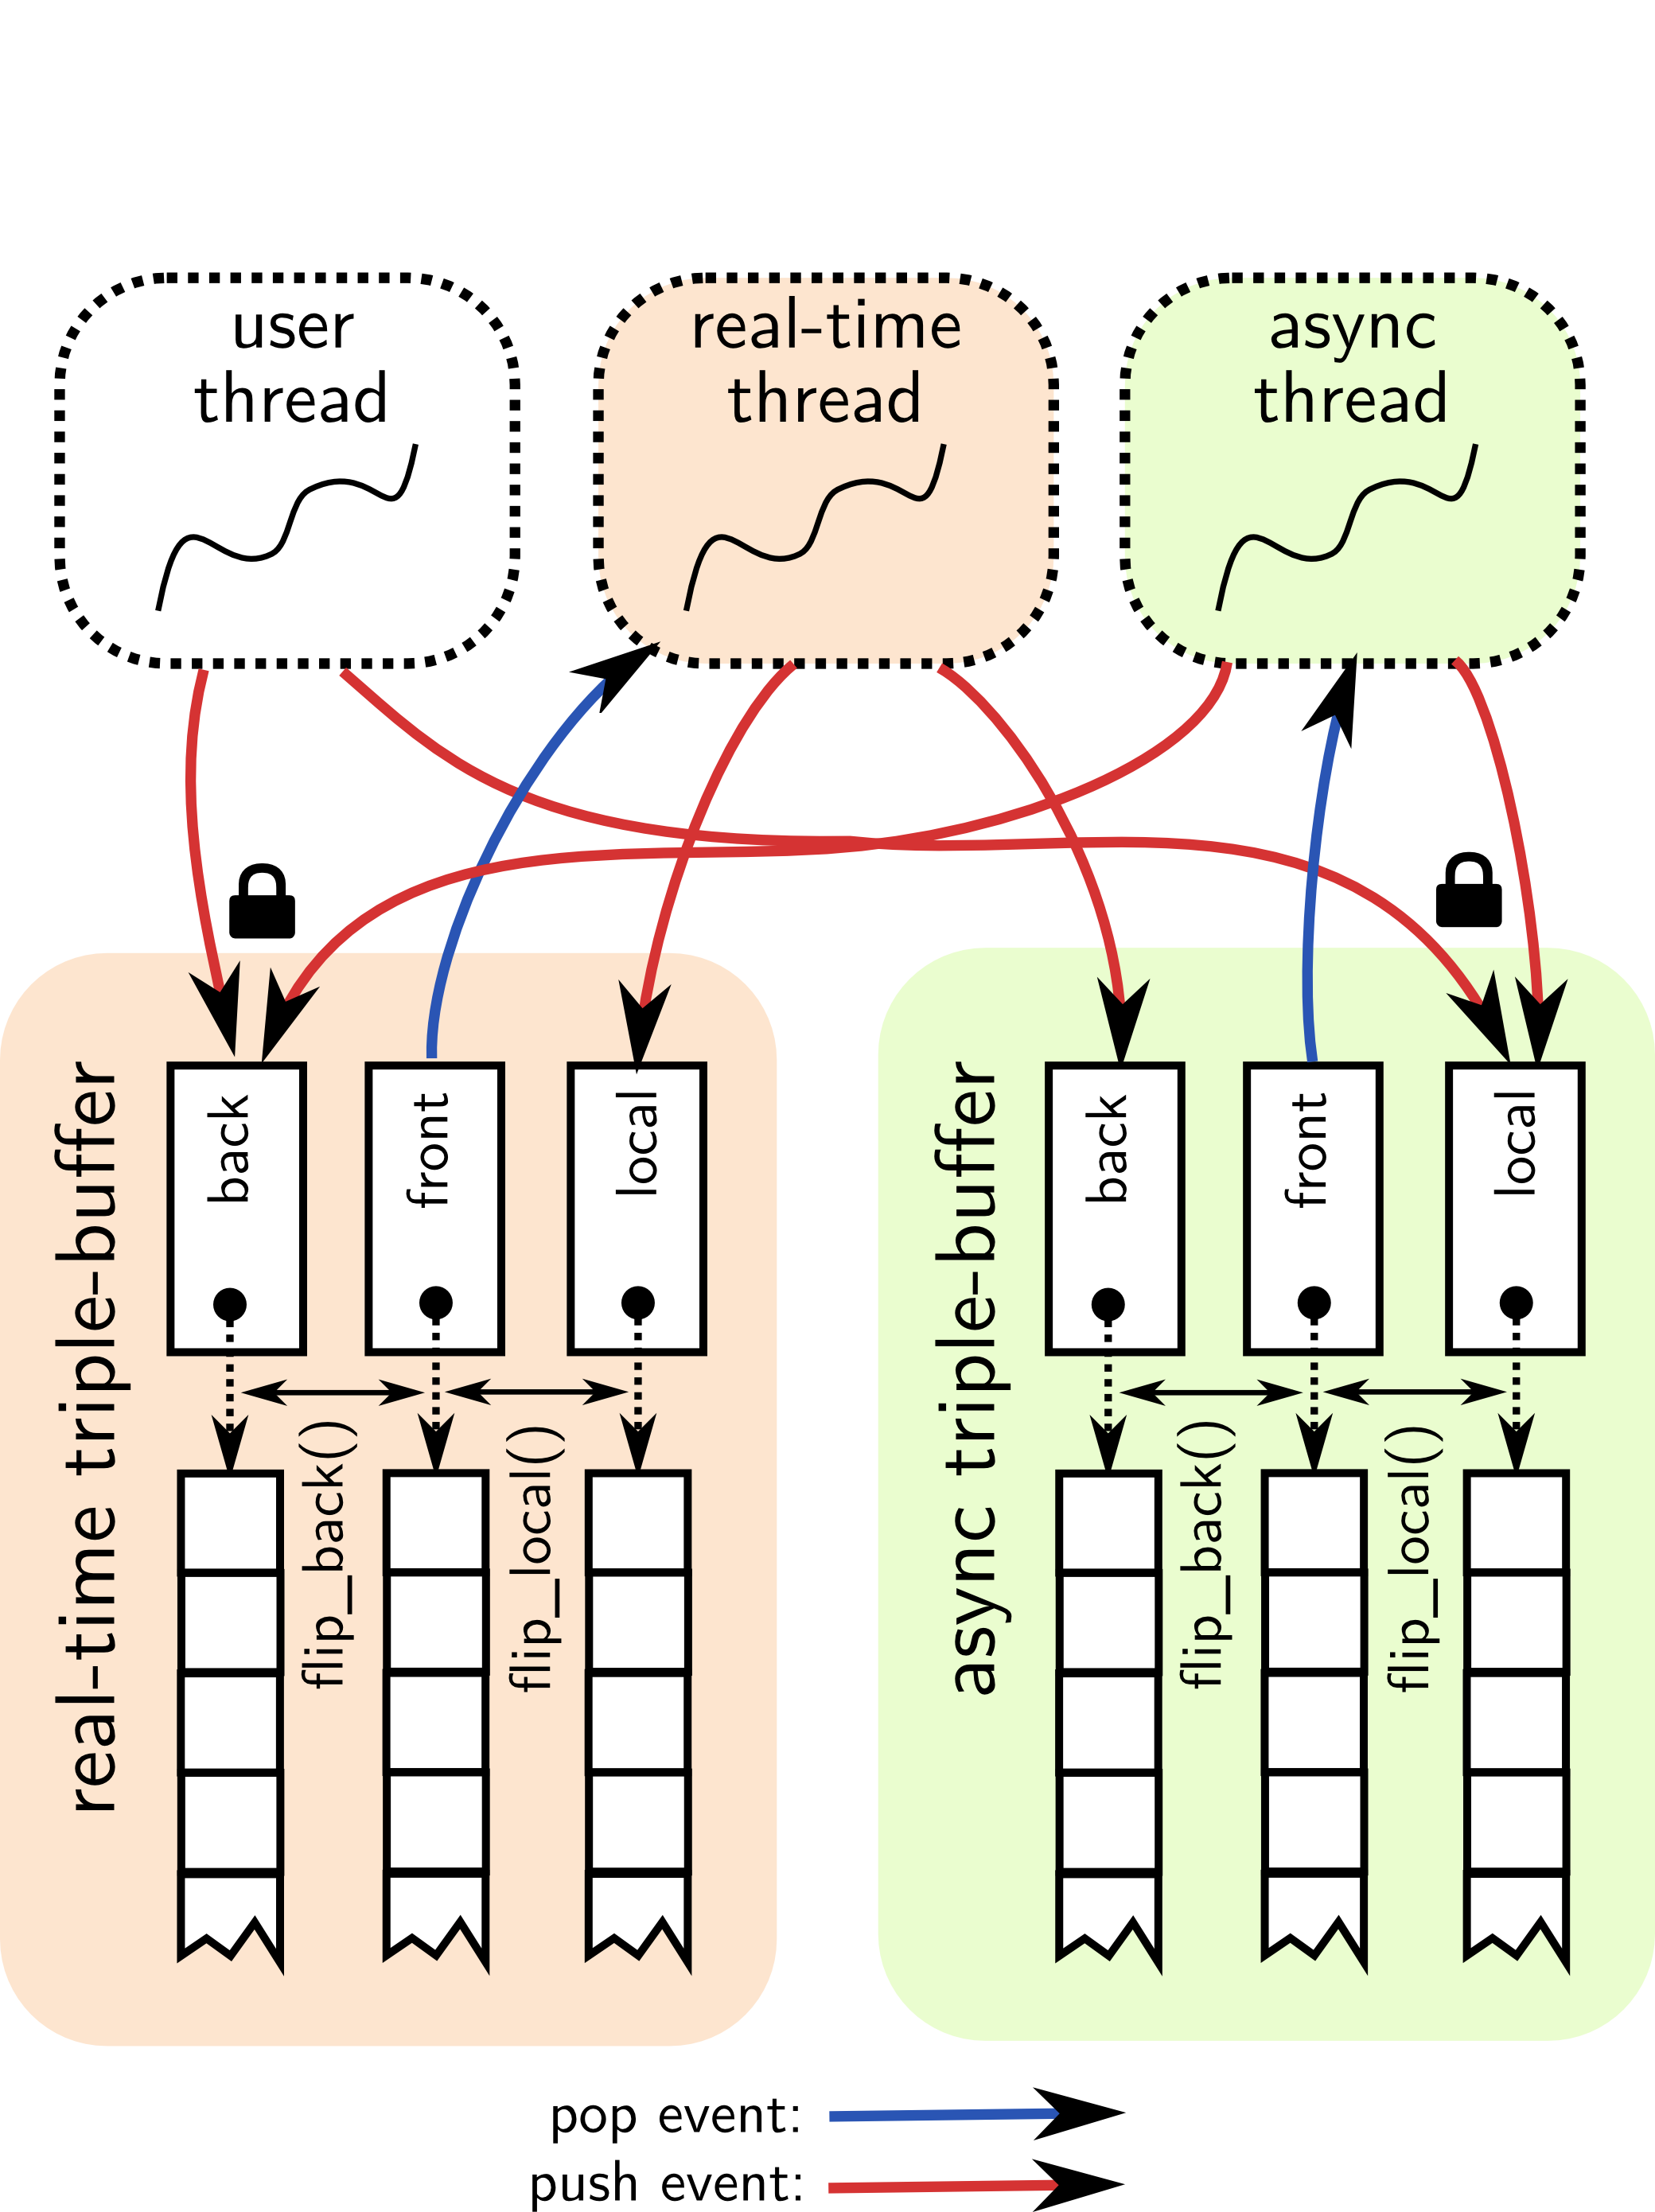
\includegraphics[width=.9\textwidth]{pic/events.png}
  \caption{Communication with triple buffer event deques.}
  \label{fig:triplebuf}
\end{figure}

\begin{description}
\item[Front buffer] This is the buffer where the events are popped
  from for processing. Only the RT thread should access the front
  of its triple buffer, and the same happens in the async thread.

\item[Back buffer] This is, in general, the buffer where events coming
  from other threads are written to. In the RT triple buffer case, the
  both the user thread and the async thread do write into it, but they
  synchronise their insertions with a mutex --- because they can! The
  \type{flip\_back ()} method exchanges the front and back
  buffers. The flip is done in the RT thread, at the beginning of each
  process request, thus should can not contend for the mutex. Instead
  it does a conditional lock, and if it fails, it skips the flip. This
  may lead to some events to be delayed more than one request if there
  is a lot of contention on the mutex --- i.e. the user and async
  threads are writing a lot of events --- but that does not happen in
  practise and informal experiments suggest that the approach is
  enough. However, this could be completely solved by implementing
  \type{hetero\_deques} lock-free at least for one writer and one
  reader, we develop this idea in section \ref{sec:improvehetero}. In
  that case, the user and async thread would still need to serialise
  their writes, but the RT can flip and read safely without caring
  about the mutex at all.

  The back of the async triple buffer is slightly different. Here,
  only the RT thread writes, because if the user thread could write on
  it at the same time we would need a lock. Indeed, it is also the RT
  thread who does the flip after filling it, as long as the async
  thread is not still processing the current front buffer, otherwise
  the flip is postponed.

\item[Local buffer] The local buffer is where a buffer writes events
  that he sends to itself. Thanks to this, we can have a notion of
  ``post-processing'' and also infinitely recursive events that
  generate a new event each time; this is very useful for implementing
  tasks and state machines. If a thread wrote his own events in its
  front buffers, this kind of behaviour would lead to an infinite loop
  and events sent to the back buffer would never be processed. The
  \type{flip\_local ()} method exchanges the front and local buffers.

  Note that in the local buffer of the async thread is a bit
  special. Because the RT thread has exclusive non synchronised access
  to the back buffer, events from the user thread are sent to the
  async thread through the local buffer, and they use a mutex to avoid
  data races.
\end{description}

While this structure might seem a bit baroque, all the complexity is
hidden in the \type{processor} and \type{*\_process\_context}
classes. In most cases, one should only care about making the right
choice of which thread should execute our event; all the complexity of
delivering and processing it is hidden and the type system ensures
we can only do it in a thread safe way.

Listing \ref{lst:nodeexample1} show an example on how to use this
event passing system. The frequency parameter is set from the user
thread, but it must be read from the RT thread and the related
variable \emph{dt} must be updated. Doing this in a portable and
thread-safe way without using mutexes is tricky. Thanks to our
structure, we just send an event that does the job of updating the
variables. There are no possible data races even if reading/writing
float values is not atomic, because the lambda expression captures a
local copy of the \type{freq} variable. This is a very convenient
fact: the event's own state provides an intermediate buffer for
communicating value updates without data races; the lambda semantics
in C++0x just provides us the syntactic sugar to make the code
pleasant to write and read. Please remember that this code is here
only to illustrate the usage of the event passing system; in practice,
passing parameters from the user thread to the RT thread is even
simpler, as we will explain in the following.


\begin{lstlisting}[float=h!, label=lst:nodeexample1, caption=A thread communication use-case]
struct example_oscillator_node : public node
{
    example_oscillator_node ()
        : _freq (440.0f) , _rt_freq (_freq), _rt_phase (0)
        , _rt_dt (0) // rt_on_context_update will be executed before
                   // the first process so we can set properly this
                   // variable that depends on the frame rate.
    
    void set_frequency (float freq) {
        _freq = freq;
        auto& ctx = process ().context ();
        ctx.push_rt_event (make_event ([=] (rt_process_context& ctx) {
            _rt_freq = freq;
            _rt_dt   = 1 / (freq * ctx.frame_rate ());
        }));
    }

    float frequency () const
    { return _freq; }

protected:
    void rt_on_context_update (rt_process_context& ctx)
    { _rt_dt = 1 / (_rt_freq * ctx.frame_rate ()); }

    void rt_do_process (rt_process_context& ctx) {
        auto frames = ctx.block_size ();
        while (frames --> 0) {
            // We suppose M_PI is defined. The output_sample function
            // does not actually exist, it is just an example.
            output_sample (std::sin (_rt_phase * 2 * M_PI));
            _rt_phase += dt;
        }
    }

    float _freq, _rt_freq;
    float _rt_phase, _rt_dt;
}
\end{lstlisting}

\subsection{Node components}

In the last section we have seen how we can easily build a notion of
\emph{parameters} similar to the one abstracted in the analysis
section on top of the event passing infrastructure. However, there are
a few ways we can criticise the approach in listing
\ref{lst:nodeexample1}:
\begin{enumerate}
\item Even though the code is not too large, in nodes with a lot of
  parameter we could easily devise a recurring pattern calling for a
  refactoring. Indeed, for passing information from the user to the
  node's processing state we do always the same: store a copy public
  for the user and another one for the node's internal processing in
  the RT thread --- to update the later from the user thread, we send
  a RT event. For controls in the other direction, this is, controls
  intended to send information from the RT thread to the user, this is
  a bit less trivial because it involves sending the update through
  the async thread and, if the status control type does not have an
  atomic assign operation, locking a mutex to avoid data races between
  the user and async thread. It seems reasonable to abstract this
  behaviour and relieve the node implementer from rewriting this
  patterns \emph{ad-nauseum}, moreover, if abstracted as a class,
  these controls can be later extended by themselves.

\item There are some corner cases that the previous code does not
  address. Actually, if the node is not attached to a processor that
  code would throw a \type{node\_attachment\_error} exception when it
  invokes the node's \type{process ()} method inside
  \type{set\_frequency ()}. It makes sense to alter the node frequency
  before attaching it anywhere so this limitation should be
  avoided. Moreover, even if the node is attached but the process is
  not started, events would accumulate in the queue. If the node is
  detached from the processor before the network is run, the internal
  frequency would never be updated indeed. This shows how there are
  many corner cases, and isolating this complexity in a class with its
  own responsibilities yields safer code.

\item Manipulating the frequency parameter as implemented in that code
  requires knowing the node's concrete type. This is a show stopper
  for the \emph{plugin} that we shall implement in the next
  iteration. Instead, parameters should be accessible directly from
  the node's basic interface, and identified with strings, such that
  using them requires no compile-time binding at all.
\end{enumerate}

This results in the notion of \emph{component}, an attribute
associated to a node, that may be of four kinds; an input port, an
output port, a input control or an output control. These four kinds of
components have different properties but there are some commonalities
among them too:
\begin{enumerate}
\item They have an unique name (unique within a node and kind of
  component) that identifies them.
\item They have an associated regular type. Regular means that it
  models the \type{Regular} concept, i.e. is default constructible,
  copy-constructible and copyable. This is the type of the data that
  they ``hold'' or ``pass''.
\item They have some associated metadata, which is just a $String
  \rightarrow String$ map providing information that may be useful to
  the user, most of the time to the human user of the application.
\item They can be queried by their name and enumerated from the node
  interface. 
\end{enumerate}

\subsubsection{Control components}

Figure \ref{fig:controls} shows the most important classes and
interfaces implementing the control components --- i.e. parameter and
status variables. Parameters or input controls are used to pass
information from the user thread to the node's internal processing
state. States or output controls work in the other way, exposing some
internal processing status to the user.

\begin{figure}[t]
  \centering
  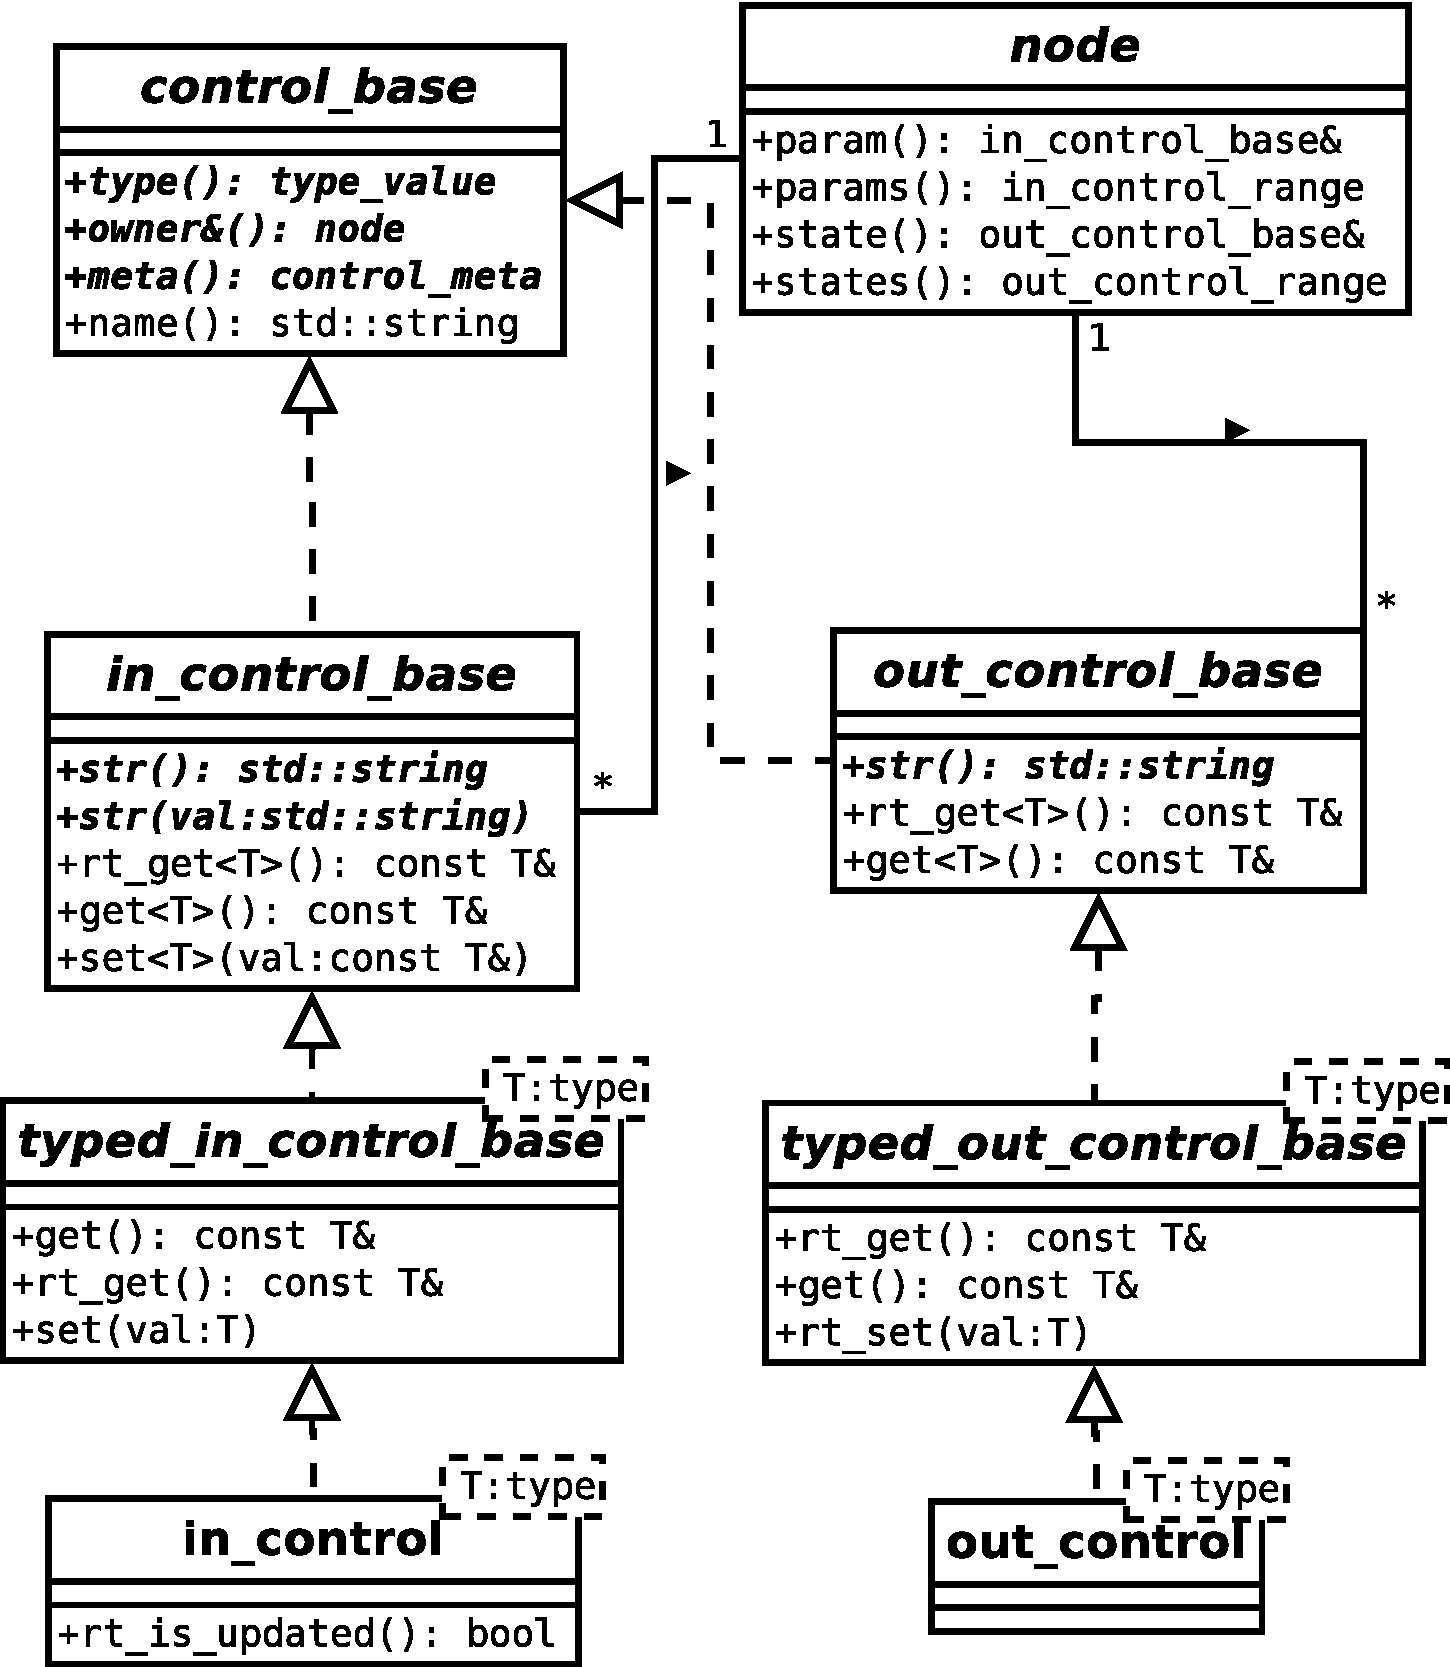
\includegraphics[width=.9\textwidth]{pic/graph-ctl.pdf}
  \caption{UML class diagram of the most important classes for the
  control components.}
\label{fig:controls}
\end{figure}

Note that in the current implementation there is some special
requirement that somehow couples the control bases and their typed
version. If you access the control through the control base access
template method with a type \type{T} and actually \type{type ()}
method returns \type{typeid (T)} for that control, then that object
must be a typed control of type $T$; otherwise this is undefined
behaviour. In practice, this means that you should never inherit from
\type{in\_control\_base} or \type{out\_control\_base} directly, but
you should inherit from their typed versions instead.

\subsection{Port components}

\label{sec:modports}

\subsection{Indirect object construction}

\label{sec:graphfactory}

\subsection{Going Model-View-Controller}

\section{Validation}

\section{Conclusion}

%%% Local Variables: 
%%% mode: latex
%%% TeX-master: "00-main"
%%% End: 


\bibliography{00-main}
\bibliographystyle{unsrt}
\addcontentsline{toc}{chapter}{Bibliography}

\startappendix

\chapter{Glossary}

\todo{¿Añado un glosario recopilando las definiciones que doy de diferentes
  términos específicos del dominio del audio y para expandir y aclarar
  siglas y acŕonimos? ¿O mejor paso? --- JP}


\chapter{Gnu General Public License}

\label{sec:license}

\begin{center}
{\parindent 0in
\textbf{Version 3, 29 June 2007}

Copyright \copyright\  2007 Free Software Foundation, Inc. \texttt{http://fsf.org/}

\bigskip
Everyone is permitted to copy and distribute verbatim copies of this

license document, but changing it is not allowed.}

\end{center}

\section{Preamble}

The GNU General Public License is a free, copyleft license for
software and other kinds of works.

The licenses for most software and other practical works are designed
to take away your freedom to share and change the works.  By contrast,
the GNU General Public License is intended to guarantee your freedom to
share and change all versions of a program--to make sure it remains free
software for all its users.  We, the Free Software Foundation, use the
GNU General Public License for most of our software; it applies also to
any other work released this way by its authors.  You can apply it to
your programs, too.

When we speak of free software, we are referring to freedom, not
price.  Our General Public Licenses are designed to make sure that you
have the freedom to distribute copies of free software (and charge for
them if you wish), that you receive source code or can get it if you
want it, that you can change the software or use pieces of it in new
free programs, and that you know you can do these things.

To protect your rights, we need to prevent others from denying you
these rights or asking you to surrender the rights.  Therefore, you have
certain responsibilities if you distribute copies of the software, or if
you modify it: responsibilities to respect the freedom of others.

For example, if you distribute copies of such a program, whether
gratis or for a fee, you must pass on to the recipients the same
freedoms that you received.  You must make sure that they, too, receive
or can get the source code.  And you must show them these terms so they
know their rights.

Developers that use the GNU GPL protect your rights with two steps:
(1) assert copyright on the software, and (2) offer you this License
giving you legal permission to copy, distribute and/or modify it.

For the developers' and authors' protection, the GPL clearly explains
that there is no warranty for this free software.  For both users' and
authors' sake, the GPL requires that modified versions be marked as
changed, so that their problems will not be attributed erroneously to
authors of previous versions.

Some devices are designed to deny users access to install or run
modified versions of the software inside them, although the manufacturer
can do so.  This is fundamentally incompatible with the aim of
protecting users' freedom to change the software.  The systematic
pattern of such abuse occurs in the area of products for individuals to
use, which is precisely where it is most unacceptable.  Therefore, we
have designed this version of the GPL to prohibit the practice for those
products.  If such problems arise substantially in other domains, we
stand ready to extend this provision to those domains in future versions
of the GPL, as needed to protect the freedom of users.

Finally, every program is threatened constantly by software patents.
States should not allow patents to restrict development and use of
software on general-purpose computers, but in those that do, we wish to
avoid the special danger that patents applied to a free program could
make it effectively proprietary.  To prevent this, the GPL assures that
patents cannot be used to render the program non-free.

The precise terms and conditions for copying, distribution and
modification follow.

\section{Terms and Conditions}

\begin{enumerate}

\addtocounter{enumi}{-1}

\item Definitions.

``This License'' refers to version 3 of the GNU General Public License.

``Copyright'' also means copyright-like laws that apply to other kinds of
works, such as semiconductor masks.

``The Program'' refers to any copyrightable work licensed under this
License.  Each licensee is addressed as ``you''.  ``Licensees'' and
``recipients'' may be individuals or organizations.

To ``modify'' a work means to copy from or adapt all or part of the work
in a fashion requiring copyright permission, other than the making of an
exact copy.  The resulting work is called a ``modified version'' of the
earlier work or a work ``based on'' the earlier work.

A ``covered work'' means either the unmodified Program or a work based
on the Program.

To ``propagate'' a work means to do anything with it that, without
permission, would make you directly or secondarily liable for
infringement under applicable copyright law, except executing it on a
computer or modifying a private copy.  Propagation includes copying,
distribution (with or without modification), making available to the
public, and in some countries other activities as well.

To ``convey'' a work means any kind of propagation that enables other
parties to make or receive copies.  Mere interaction with a user through
a computer network, with no transfer of a copy, is not conveying.

An interactive user interface displays ``Appropriate Legal Notices''
to the extent that it includes a convenient and prominently visible
feature that (1) displays an appropriate copyright notice, and (2)
tells the user that there is no warranty for the work (except to the
extent that warranties are provided), that licensees may convey the
work under this License, and how to view a copy of this License.  If
the interface presents a list of user commands or options, such as a
menu, a prominent item in the list meets this criterion.

\item Source Code.

The ``source code'' for a work means the preferred form of the work
for making modifications to it.  ``Object code'' means any non-source
form of a work.

A ``Standard Interface'' means an interface that either is an official
standard defined by a recognized standards body, or, in the case of
interfaces specified for a particular programming language, one that
is widely used among developers working in that language.

The ``System Libraries'' of an executable work include anything, other
than the work as a whole, that (a) is included in the normal form of
packaging a Major Component, but which is not part of that Major
Component, and (b) serves only to enable use of the work with that
Major Component, or to implement a Standard Interface for which an
implementation is available to the public in source code form.  A
``Major Component'', in this context, means a major essential component
(kernel, window system, and so on) of the specific operating system
(if any) on which the executable work runs, or a compiler used to
produce the work, or an object code interpreter used to run it.

The ``Corresponding Source'' for a work in object code form means all
the source code needed to generate, install, and (for an executable
work) run the object code and to modify the work, including scripts to
control those activities.  However, it does not include the work's
System Libraries, or general-purpose tools or generally available free
programs which are used unmodified in performing those activities but
which are not part of the work.  For example, Corresponding Source
includes interface definition files associated with source files for
the work, and the source code for shared libraries and dynamically
linked subprograms that the work is specifically designed to require,
such as by intimate data communication or control flow between those
subprograms and other parts of the work.

The Corresponding Source need not include anything that users
can regenerate automatically from other parts of the Corresponding
Source.

The Corresponding Source for a work in source code form is that
same work.

\item Basic Permissions.

All rights granted under this License are granted for the term of
copyright on the Program, and are irrevocable provided the stated
conditions are met.  This License explicitly affirms your unlimited
permission to run the unmodified Program.  The output from running a
covered work is covered by this License only if the output, given its
content, constitutes a covered work.  This License acknowledges your
rights of fair use or other equivalent, as provided by copyright law.

You may make, run and propagate covered works that you do not
convey, without conditions so long as your license otherwise remains
in force.  You may convey covered works to others for the sole purpose
of having them make modifications exclusively for you, or provide you
with facilities for running those works, provided that you comply with
the terms of this License in conveying all material for which you do
not control copyright.  Those thus making or running the covered works
for you must do so exclusively on your behalf, under your direction
and control, on terms that prohibit them from making any copies of
your copyrighted material outside their relationship with you.

Conveying under any other circumstances is permitted solely under
the conditions stated below.  Sublicensing is not allowed; section 10
makes it unnecessary.

\item Protecting Users' Legal Rights From Anti-Circumvention Law.

No covered work shall be deemed part of an effective technological
measure under any applicable law fulfilling obligations under article
11 of the WIPO copyright treaty adopted on 20 December 1996, or
similar laws prohibiting or restricting circumvention of such
measures.

When you convey a covered work, you waive any legal power to forbid
circumvention of technological measures to the extent such circumvention
is effected by exercising rights under this License with respect to
the covered work, and you disclaim any intention to limit operation or
modification of the work as a means of enforcing, against the work's
users, your or third parties' legal rights to forbid circumvention of
technological measures.

\item Conveying Verbatim Copies.

You may convey verbatim copies of the Program's source code as you
receive it, in any medium, provided that you conspicuously and
appropriately publish on each copy an appropriate copyright notice;
keep intact all notices stating that this License and any
non-permissive terms added in accord with section 7 apply to the code;
keep intact all notices of the absence of any warranty; and give all
recipients a copy of this License along with the Program.

You may charge any price or no price for each copy that you convey,
and you may offer support or warranty protection for a fee.

\item Conveying Modified Source Versions.

You may convey a work based on the Program, or the modifications to
produce it from the Program, in the form of source code under the
terms of section 4, provided that you also meet all of these conditions:
  \begin{enumerate}
  \item The work must carry prominent notices stating that you modified
  it, and giving a relevant date.

  \item The work must carry prominent notices stating that it is
  released under this License and any conditions added under section
  7.  This requirement modifies the requirement in section 4 to
  ``keep intact all notices''.

  \item You must license the entire work, as a whole, under this
  License to anyone who comes into possession of a copy.  This
  License will therefore apply, along with any applicable section 7
  additional terms, to the whole of the work, and all its parts,
  regardless of how they are packaged.  This License gives no
  permission to license the work in any other way, but it does not
  invalidate such permission if you have separately received it.

  \item If the work has interactive user interfaces, each must display
  Appropriate Legal Notices; however, if the Program has interactive
  interfaces that do not display Appropriate Legal Notices, your
  work need not make them do so.
\end{enumerate}
A compilation of a covered work with other separate and independent
works, which are not by their nature extensions of the covered work,
and which are not combined with it such as to form a larger program,
in or on a volume of a storage or distribution medium, is called an
``aggregate'' if the compilation and its resulting copyright are not
used to limit the access or legal rights of the compilation's users
beyond what the individual works permit.  Inclusion of a covered work
in an aggregate does not cause this License to apply to the other
parts of the aggregate.

\item Conveying Non-Source Forms.

You may convey a covered work in object code form under the terms
of sections 4 and 5, provided that you also convey the
machine-readable Corresponding Source under the terms of this License,
in one of these ways:
  \begin{enumerate}
  \item Convey the object code in, or embodied in, a physical product
  (including a physical distribution medium), accompanied by the
  Corresponding Source fixed on a durable physical medium
  customarily used for software interchange.

  \item Convey the object code in, or embodied in, a physical product
  (including a physical distribution medium), accompanied by a
  written offer, valid for at least three years and valid for as
  long as you offer spare parts or customer support for that product
  model, to give anyone who possesses the object code either (1) a
  copy of the Corresponding Source for all the software in the
  product that is covered by this License, on a durable physical
  medium customarily used for software interchange, for a price no
  more than your reasonable cost of physically performing this
  conveying of source, or (2) access to copy the
  Corresponding Source from a network server at no charge.

  \item Convey individual copies of the object code with a copy of the
  written offer to provide the Corresponding Source.  This
  alternative is allowed only occasionally and noncommercially, and
  only if you received the object code with such an offer, in accord
  with subsection 6b.

  \item Convey the object code by offering access from a designated
  place (gratis or for a charge), and offer equivalent access to the
  Corresponding Source in the same way through the same place at no
  further charge.  You need not require recipients to copy the
  Corresponding Source along with the object code.  If the place to
  copy the object code is a network server, the Corresponding Source
  may be on a different server (operated by you or a third party)
  that supports equivalent copying facilities, provided you maintain
  clear directions next to the object code saying where to find the
  Corresponding Source.  Regardless of what server hosts the
  Corresponding Source, you remain obligated to ensure that it is
  available for as long as needed to satisfy these requirements.

  \item Convey the object code using peer-to-peer transmission, provided
  you inform other peers where the object code and Corresponding
  Source of the work are being offered to the general public at no
  charge under subsection 6d.
  \end{enumerate}

A separable portion of the object code, whose source code is excluded
from the Corresponding Source as a System Library, need not be
included in conveying the object code work.

A ``User Product'' is either (1) a ``consumer product'', which means any
tangible personal property which is normally used for personal, family,
or household purposes, or (2) anything designed or sold for incorporation
into a dwelling.  In determining whether a product is a consumer product,
doubtful cases shall be resolved in favor of coverage.  For a particular
product received by a particular user, ``normally used'' refers to a
typical or common use of that class of product, regardless of the status
of the particular user or of the way in which the particular user
actually uses, or expects or is expected to use, the product.  A product
is a consumer product regardless of whether the product has substantial
commercial, industrial or non-consumer uses, unless such uses represent
the only significant mode of use of the product.

``Installation Information'' for a User Product means any methods,
procedures, authorization keys, or other information required to install
and execute modified versions of a covered work in that User Product from
a modified version of its Corresponding Source.  The information must
suffice to ensure that the continued functioning of the modified object
code is in no case prevented or interfered with solely because
modification has been made.

If you convey an object code work under this section in, or with, or
specifically for use in, a User Product, and the conveying occurs as
part of a transaction in which the right of possession and use of the
User Product is transferred to the recipient in perpetuity or for a
fixed term (regardless of how the transaction is characterized), the
Corresponding Source conveyed under this section must be accompanied
by the Installation Information.  But this requirement does not apply
if neither you nor any third party retains the ability to install
modified object code on the User Product (for example, the work has
been installed in ROM).

The requirement to provide Installation Information does not include a
requirement to continue to provide support service, warranty, or updates
for a work that has been modified or installed by the recipient, or for
the User Product in which it has been modified or installed.  Access to a
network may be denied when the modification itself materially and
adversely affects the operation of the network or violates the rules and
protocols for communication across the network.

Corresponding Source conveyed, and Installation Information provided,
in accord with this section must be in a format that is publicly
documented (and with an implementation available to the public in
source code form), and must require no special password or key for
unpacking, reading or copying.

\item Additional Terms.

``Additional permissions'' are terms that supplement the terms of this
License by making exceptions from one or more of its conditions.
Additional permissions that are applicable to the entire Program shall
be treated as though they were included in this License, to the extent
that they are valid under applicable law.  If additional permissions
apply only to part of the Program, that part may be used separately
under those permissions, but the entire Program remains governed by
this License without regard to the additional permissions.

When you convey a copy of a covered work, you may at your option
remove any additional permissions from that copy, or from any part of
it.  (Additional permissions may be written to require their own
removal in certain cases when you modify the work.)  You may place
additional permissions on material, added by you to a covered work,
for which you have or can give appropriate copyright permission.

Notwithstanding any other provision of this License, for material you
add to a covered work, you may (if authorized by the copyright holders of
that material) supplement the terms of this License with terms:
  \begin{enumerate}
  \item Disclaiming warranty or limiting liability differently from the
  terms of sections 15 and 16 of this License; or

  \item Requiring preservation of specified reasonable legal notices or
  author attributions in that material or in the Appropriate Legal
  Notices displayed by works containing it; or

  \item Prohibiting misrepresentation of the origin of that material, or
  requiring that modified versions of such material be marked in
  reasonable ways as different from the original version; or

  \item Limiting the use for publicity purposes of names of licensors or
  authors of the material; or

  \item Declining to grant rights under trademark law for use of some
  trade names, trademarks, or service marks; or

  \item Requiring indemnification of licensors and authors of that
  material by anyone who conveys the material (or modified versions of
  it) with contractual assumptions of liability to the recipient, for
  any liability that these contractual assumptions directly impose on
  those licensors and authors.
  \end{enumerate}

All other non-permissive additional terms are considered ``further
restrictions'' within the meaning of section 10.  If the Program as you
received it, or any part of it, contains a notice stating that it is
governed by this License along with a term that is a further
restriction, you may remove that term.  If a license document contains
a further restriction but permits relicensing or conveying under this
License, you may add to a covered work material governed by the terms
of that license document, provided that the further restriction does
not survive such relicensing or conveying.

If you add terms to a covered work in accord with this section, you
must place, in the relevant source files, a statement of the
additional terms that apply to those files, or a notice indicating
where to find the applicable terms.

Additional terms, permissive or non-permissive, may be stated in the
form of a separately written license, or stated as exceptions;
the above requirements apply either way.

\item Termination.

You may not propagate or modify a covered work except as expressly
provided under this License.  Any attempt otherwise to propagate or
modify it is void, and will automatically terminate your rights under
this License (including any patent licenses granted under the third
paragraph of section 11).

However, if you cease all violation of this License, then your
license from a particular copyright holder is reinstated (a)
provisionally, unless and until the copyright holder explicitly and
finally terminates your license, and (b) permanently, if the copyright
holder fails to notify you of the violation by some reasonable means
prior to 60 days after the cessation.

Moreover, your license from a particular copyright holder is
reinstated permanently if the copyright holder notifies you of the
violation by some reasonable means, this is the first time you have
received notice of violation of this License (for any work) from that
copyright holder, and you cure the violation prior to 30 days after
your receipt of the notice.

Termination of your rights under this section does not terminate the
licenses of parties who have received copies or rights from you under
this License.  If your rights have been terminated and not permanently
reinstated, you do not qualify to receive new licenses for the same
material under section 10.

\item Acceptance Not Required for Having Copies.

You are not required to accept this License in order to receive or
run a copy of the Program.  Ancillary propagation of a covered work
occurring solely as a consequence of using peer-to-peer transmission
to receive a copy likewise does not require acceptance.  However,
nothing other than this License grants you permission to propagate or
modify any covered work.  These actions infringe copyright if you do
not accept this License.  Therefore, by modifying or propagating a
covered work, you indicate your acceptance of this License to do so.

\item Automatic Licensing of Downstream Recipients.

Each time you convey a covered work, the recipient automatically
receives a license from the original licensors, to run, modify and
propagate that work, subject to this License.  You are not responsible
for enforcing compliance by third parties with this License.

An ``entity transaction'' is a transaction transferring control of an
organization, or substantially all assets of one, or subdividing an
organization, or merging organizations.  If propagation of a covered
work results from an entity transaction, each party to that
transaction who receives a copy of the work also receives whatever
licenses to the work the party's predecessor in interest had or could
give under the previous paragraph, plus a right to possession of the
Corresponding Source of the work from the predecessor in interest, if
the predecessor has it or can get it with reasonable efforts.

You may not impose any further restrictions on the exercise of the
rights granted or affirmed under this License.  For example, you may
not impose a license fee, royalty, or other charge for exercise of
rights granted under this License, and you may not initiate litigation
(including a cross-claim or counterclaim in a lawsuit) alleging that
any patent claim is infringed by making, using, selling, offering for
sale, or importing the Program or any portion of it.

\item Patents.

A ``contributor'' is a copyright holder who authorizes use under this
License of the Program or a work on which the Program is based.  The
work thus licensed is called the contributor's ``contributor version''.

A contributor's ``essential patent claims'' are all patent claims
owned or controlled by the contributor, whether already acquired or
hereafter acquired, that would be infringed by some manner, permitted
by this License, of making, using, or selling its contributor version,
but do not include claims that would be infringed only as a
consequence of further modification of the contributor version.  For
purposes of this definition, ``control'' includes the right to grant
patent sublicenses in a manner consistent with the requirements of
this License.

Each contributor grants you a non-exclusive, worldwide, royalty-free
patent license under the contributor's essential patent claims, to
make, use, sell, offer for sale, import and otherwise run, modify and
propagate the contents of its contributor version.

In the following three paragraphs, a ``patent license'' is any express
agreement or commitment, however denominated, not to enforce a patent
(such as an express permission to practice a patent or covenant not to
sue for patent infringement).  To ``grant'' such a patent license to a
party means to make such an agreement or commitment not to enforce a
patent against the party.

If you convey a covered work, knowingly relying on a patent license,
and the Corresponding Source of the work is not available for anyone
to copy, free of charge and under the terms of this License, through a
publicly available network server or other readily accessible means,
then you must either (1) cause the Corresponding Source to be so
available, or (2) arrange to deprive yourself of the benefit of the
patent license for this particular work, or (3) arrange, in a manner
consistent with the requirements of this License, to extend the patent
license to downstream recipients.  ``Knowingly relying'' means you have
actual knowledge that, but for the patent license, your conveying the
covered work in a country, or your recipient's use of the covered work
in a country, would infringe one or more identifiable patents in that
country that you have reason to believe are valid.

If, pursuant to or in connection with a single transaction or
arrangement, you convey, or propagate by procuring conveyance of, a
covered work, and grant a patent license to some of the parties
receiving the covered work authorizing them to use, propagate, modify
or convey a specific copy of the covered work, then the patent license
you grant is automatically extended to all recipients of the covered
work and works based on it.

A patent license is ``discriminatory'' if it does not include within
the scope of its coverage, prohibits the exercise of, or is
conditioned on the non-exercise of one or more of the rights that are
specifically granted under this License.  You may not convey a covered
work if you are a party to an arrangement with a third party that is
in the business of distributing software, under which you make payment
to the third party based on the extent of your activity of conveying
the work, and under which the third party grants, to any of the
parties who would receive the covered work from you, a discriminatory
patent license (a) in connection with copies of the covered work
conveyed by you (or copies made from those copies), or (b) primarily
for and in connection with specific products or compilations that
contain the covered work, unless you entered into that arrangement,
or that patent license was granted, prior to 28 March 2007.

Nothing in this License shall be construed as excluding or limiting
any implied license or other defenses to infringement that may
otherwise be available to you under applicable patent law.

\item No Surrender of Others' Freedom.

If conditions are imposed on you (whether by court order, agreement or
otherwise) that contradict the conditions of this License, they do not
excuse you from the conditions of this License.  If you cannot convey a
covered work so as to satisfy simultaneously your obligations under this
License and any other pertinent obligations, then as a consequence you may
not convey it at all.  For example, if you agree to terms that obligate you
to collect a royalty for further conveying from those to whom you convey
the Program, the only way you could satisfy both those terms and this
License would be to refrain entirely from conveying the Program.

\item Use with the GNU Affero General Public License.

Notwithstanding any other provision of this License, you have
permission to link or combine any covered work with a work licensed
under version 3 of the GNU Affero General Public License into a single
combined work, and to convey the resulting work.  The terms of this
License will continue to apply to the part which is the covered work,
but the special requirements of the GNU Affero General Public License,
section 13, concerning interaction through a network will apply to the
combination as such.

\item Revised Versions of this License.

The Free Software Foundation may publish revised and/or new versions of
the GNU General Public License from time to time.  Such new versions will
be similar in spirit to the present version, but may differ in detail to
address new problems or concerns.

Each version is given a distinguishing version number.  If the
Program specifies that a certain numbered version of the GNU General
Public License ``or any later version'' applies to it, you have the
option of following the terms and conditions either of that numbered
version or of any later version published by the Free Software
Foundation.  If the Program does not specify a version number of the
GNU General Public License, you may choose any version ever published
by the Free Software Foundation.

If the Program specifies that a proxy can decide which future
versions of the GNU General Public License can be used, that proxy's
public statement of acceptance of a version permanently authorizes you
to choose that version for the Program.

Later license versions may give you additional or different
permissions.  However, no additional obligations are imposed on any
author or copyright holder as a result of your choosing to follow a
later version.

\item Disclaimer of Warranty.

\begin{sloppypar}
 THERE IS NO WARRANTY FOR THE PROGRAM, TO THE EXTENT PERMITTED BY
 APPLICABLE LAW.  EXCEPT WHEN OTHERWISE STATED IN WRITING THE
 COPYRIGHT HOLDERS AND/OR OTHER PARTIES PROVIDE THE PROGRAM ``AS IS''
 WITHOUT WARRANTY OF ANY KIND, EITHER EXPRESSED OR IMPLIED,
 INCLUDING, BUT NOT LIMITED TO, THE IMPLIED WARRANTIES OF
 MERCHANTABILITY AND FITNESS FOR A PARTICULAR PURPOSE.  THE ENTIRE
 RISK AS TO THE QUALITY AND PERFORMANCE OF THE PROGRAM IS WITH YOU.
 SHOULD THE PROGRAM PROVE DEFECTIVE, YOU ASSUME THE COST OF ALL
 NECESSARY SERVICING, REPAIR OR CORRECTION.
\end{sloppypar}

\item Limitation of Liability.

 IN NO EVENT UNLESS REQUIRED BY APPLICABLE LAW OR AGREED TO IN
 WRITING WILL ANY COPYRIGHT HOLDER, OR ANY OTHER PARTY WHO MODIFIES
 AND/OR CONVEYS THE PROGRAM AS PERMITTED ABOVE, BE LIABLE TO YOU FOR
 DAMAGES, INCLUDING ANY GENERAL, SPECIAL, INCIDENTAL OR CONSEQUENTIAL
 DAMAGES ARISING OUT OF THE USE OR INABILITY TO USE THE PROGRAM
 (INCLUDING BUT NOT LIMITED TO LOSS OF DATA OR DATA BEING RENDERED
 INACCURATE OR LOSSES SUSTAINED BY YOU OR THIRD PARTIES OR A FAILURE
 OF THE PROGRAM TO OPERATE WITH ANY OTHER PROGRAMS), EVEN IF SUCH
 HOLDER OR OTHER PARTY HAS BEEN ADVISED OF THE POSSIBILITY OF SUCH
 DAMAGES.

\item Interpretation of Sections 15 and 16.

If the disclaimer of warranty and limitation of liability provided
above cannot be given local legal effect according to their terms,
reviewing courts shall apply local law that most closely approximates
an absolute waiver of all civil liability in connection with the
Program, unless a warranty or assumption of liability accompanies a
copy of the Program in return for a fee.

\begin{center}
{\Large\sc End of Terms and Conditions}

\bigskip
How to Apply These Terms to Your New Programs
\end{center}

If you develop a new program, and you want it to be of the greatest
possible use to the public, the best way to achieve this is to make it
free software which everyone can redistribute and change under these terms.

To do so, attach the following notices to the program.  It is safest
to attach them to the start of each source file to most effectively
state the exclusion of warranty; and each file should have at least
the ``copyright'' line and a pointer to where the full notice is found.

{\footnotesize
\begin{verbatim}
<one line to give the program's name and a brief idea of what it does.>

Copyright (C) <textyear>  <name of author>

This program is free software: you can redistribute it and/or modify
it under the terms of the GNU General Public License as published by
the Free Software Foundation, either version 3 of the License, or
(at your option) any later version.

This program is distributed in the hope that it will be useful,
but WITHOUT ANY WARRANTY; without even the implied warranty of
MERCHANTABILITY or FITNESS FOR A PARTICULAR PURPOSE.  See the
GNU General Public License for more details.

You should have received a copy of the GNU General Public License
along with this program.  If not, see <http://www.gnu.org/licenses/>.
\end{verbatim}
}

Also add information on how to contact you by electronic and paper mail.

If the program does terminal interaction, make it output a short
notice like this when it starts in an interactive mode:

{\footnotesize
\begin{verbatim}
<program>  Copyright (C) <year>  <name of author>

This program comes with ABSOLUTELY NO WARRANTY; for details type `show w'.
This is free software, and you are welcome to redistribute it
under certain conditions; type `show c' for details.
\end{verbatim}
}

The hypothetical commands {\tt show w} and {\tt show c} should show
the appropriate
parts of the General Public License.  Of course, your program's commands
might be different; for a GUI interface, you would use an ``about box''.

You should also get your employer (if you work as a programmer) or
school, if any, to sign a ``copyright disclaimer'' for the program, if
necessary.  For more information on this, and how to apply and follow
the GNU GPL, see \texttt{http://www.gnu.org/licenses/}.

The GNU General Public License does not permit incorporating your
program into proprietary programs.  If your program is a subroutine
library, you may consider it more useful to permit linking proprietary
applications with the library.  If this is what you want to do, use
the GNU Lesser General Public License instead of this License.  But
first, please read: \\\texttt{http://www.gnu.org/philosophy/why-not-lgpl.html}.

\end{enumerate}

%%% Local Variables: 
%%% mode: latex
%%% TeX-master: "00-main"
%%% End: 


\end{document}

%%% Local Variables: 
%%% mode: latex
%%% TeX-master: t
%%% End: 
